\documentclass{article}

% Use numeric citations with natbib.
\PassOptionsToPackage{numbers, compress}{natbib}

% NeurIPS 2026 template.
% For submission, keep the default option below. For camera-ready, use e.g.
% \usepackage[main, final]{neurips_2026}
% For arXiv/preprint, use \usepackage[preprint]{neurips_2026}
\usepackage[preprint]{neurips_2026}

% Standard NeurIPS/sample-template packages
\usepackage[utf8]{inputenc}
\usepackage[T1]{fontenc}
\usepackage{hyperref}
\usepackage{url}
\usepackage{booktabs}
\usepackage{amsfonts}
\usepackage{nicefrac}
\usepackage{microtype}
\usepackage[table]{xcolor}
\usepackage{wrapfig}
\usepackage[most]{tcolorbox}



% Packages from the original main.tex
\usepackage{graphicx}
\usepackage{subcaption}
\usepackage{amsmath}
\usepackage{amssymb}
\usepackage{mathtools}
\usepackage{amsthm}
\usepackage{enumitem}
\usepackage{tabularx}
\usepackage[capitalize,noabbrev]{cleveref}
\usepackage{bm}
\usepackage{algorithm}
\usepackage{algpseudocode}
\usepackage{multirow}
\usepackage{dsfont}
\usepackage{soul}
\usepackage[textsize=tiny]{todonotes}
\definecolor{bestgreen}{RGB}{220,245,220}
\definecolor{lightred}{RGB}{255,225,225}
\definecolor{lightyellow}{RGB}{255,245,200}
\definecolor{lightblue}{RGB}{225,240,255}


\newtcolorbox{highlightbox}{
  enhanced,
  breakable,
  colback=lightblue,
  colframe=blue!0!black,
  boxrule=0.8pt,
  arc=7pt,
  left=7pt,
  right=7pt,
  top=7pt,
  bottom=7pt,
  before skip=10pt,
  after skip=10pt
}

\allowdisplaybreaks

\newtcolorbox{chatbox}{
    colback=gray!5!white,
    colframe=gray!75!black,
    arc=5pt,
    boxrule=0.5pt,
    left=5pt,
    right=5pt,
    top=5pt,
    bottom=5pt,
    fontupper=\ttfamily\small
}

% Attempt to make hyperref and algorithmic work together better.
% \newcommand{\theHalgorithm}{\arabic{algorithm}}

%%%%%%%%%%%%%%%%%%%%%%%%%%%%%%%%
% THEOREMS
%%%%%%%%%%%%%%%%%%%%%%%%%%%%%%%%
\theoremstyle{plain}
\newtheorem{theorem}{Theorem}[section]
\newtheorem{proposition}[theorem]{Proposition}
\newtheorem{lemma}[theorem]{Lemma}
\newtheorem{corollary}[theorem]{Corollary}
\theoremstyle{definition}
\newtheorem{definition}[theorem]{Definition}
\newtheorem{assumption}[theorem]{Assumption}
\theoremstyle{remark}
\newtheorem{remark}[theorem]{Remark}


% common notations
\newcommand{\one}{\bm 1}
\newcommand{\zero}{\textbf{0}}
\newcommand{\e}{{\bm e}}
\newcommand{\Var}{\mathsf{Var}}
\newcommand{\LL}{\mathcal L}
\newcommand{\Cov}{\mathrm{Cov}}
\newcommand{\U}{\mathrm{Unit}}
\newcommand{\bdiag}{\mathrm{bdiag}}
\newcommand{\EE}{\mathbb{E}}
\newcommand{\PP}{\mathbb{P}}
\newcommand{\QQ}{\mathbb{Q}}
\newcommand{\nm}[1]{\left\|{#1}\right\|}
\newcommand{\ra}{\rightarrow}
\newcommand{\R}{\mathbb{R}}
\newcommand{\ip}[1]{\left<{#1}\right>}
\newcommand{\eqbr}{\phantom{{}=1}}
\newcommand{\avg}[1]{\frac{1}{#1}\sum_{i=1}^{#1}}

% transformers
\newcommand{\WQK}[1]{\bm W_\mathrm{QK}^{({#1})}}
\newcommand{\WOV}[1]{\bm W_\mathrm{OV}^{({#1})}}
\newcommand{\Att}[2]{\sigma\left(\frac{{#1}{#2}{#1}^\top}{\sqrt{d}}\right)}
\newcommand{\fd}[2]{\frac{\partial{#1}}{\partial{#2}}}
\newcommand{\sd}[2]{\frac{\partial^2{#1}}{\partial{#2}^2}}
\newcommand{\vecr}{\mathrm{vec}_\mathrm{r}}
\newcommand{\vecc}{\mathrm{vec}_\mathrm{c}}
\newcommand{\mask}{\texttt{M}}
\newcommand{\alg}{VLP}

\algnewcommand{\Input}{\item[\textbf{Input:}]}
\algnewcommand{\Output}{\item[\textbf{Output:}]}

\DeclareMathOperator*{\argmin}{argmin}
\DeclareMathOperator*{\argmax}{argmax}
\DeclareMathOperator{\prox}{prox}
\DeclareMathOperator{\proj}{proj}
\DeclareMathOperator{\dom}{dom}
\DeclareMathOperator{\tr}{tr}
\DeclareMathOperator{\Det}{Det}
\DeclareMathOperator{\diag}{diag}
\DeclareMathOperator{\Diag}{Diag}
\DeclareMathOperator{\Rank}{Rank}
\DeclareMathOperator{\spn}{span}
\DeclareMathOperator{\sgn}{sgn}
\DeclareMathOperator{\ind}{\mathds{1}}

\def\vx{{\bm{x}}}
\def\vy{{\bm{y}}}
\def\vs{{\bm{s}}}

% Author comments
\newcommand{\jk}[1]{\textcolor{red}{Jason: #1}}
\newcommand{\sijin}[1]{\textcolor{blue}{[Sijin: #1]}}
\newcommand{\cy}[1]{\textcolor{green}{Chang: #1}}
\newcommand{\jiaxin}[1]{\textcolor{blue}{[Jiaxin: #1]}}
\newcommand{\strblk}[1]{\sethlcolor{black!12}\hl{\texttt{\footnotesize #1}}}

\title{On Confidence-Based Decoding Strategies for Masked Diffusion and Beyond: A Likelihood Optimization Perspective}

% In the default NeurIPS submission mode, the style anonymizes author information.
% For the camera-ready version, compile with the final option above.
\author{%
  Sijin Chen \\
  Princeton University \\
  \texttt{chensj@princeton.edu}
  \And
  Chang Yu \\
  Princeton University \\
  \texttt{cy7438@princeton.edu}
  \And
  Jiaxin Shi \\
  Meta SuperIntelligence Labs
  \And
  Jason M. Klusowski \\
  Princeton University \\
  \texttt{jason.klusowski@princeton.edu}
}

\begin{document}

\maketitle

\begin{abstract}
Masked diffusion language models enable a more flexible generation order than their autoregressive counterparts, but raise the question of what unmasking order is optimal during sampling. Empirically, confidence-based unmasking heuristics perform strongly in practice, but the theoretical basis for their advantages remains unclear. In this work, we develop a theoretical account of confidence-based methods by studying a likelihood optimization problem that searches for the best unmasking policy to maximize sample likelihood. Under planning-depth reduction and distribution approximation, we show that confidence unmasking emerges as the (near-)optimal policy in our framework, justifying its empirical superiority. Building on the likelihood principle, we further propose a trainable policy that learns to optimize the global objective without the previous simplifications. Across experiments on multiple MDMs of different scales spanning text, code, and math generation benchmarks, the trained policy matches or exceeds the performance of confidence-based methods. Overall, our work demonstrates the potential of a likelihood optimization framework for analyzing and developing efficient sampling methods for diffusion language models.
\end{abstract}

\iffalse
\jk{[\S5.1] The ELBO/KL decomposition seems to take a KL against an \emph{unnormalized} quantity over $U$ (via $\rho^{\theta,\pi}_0$). It may read more cleanly (and be formally correct) if rewritten using the standard identity with a normalized posterior, e.g., $\mathrm{KL}(w(U)\,\|\,p(U\mid x_0))$.}


\jk{[Alg.~1--2 vs. main text] The algorithms use $p^\theta_{t_k}(\cdot\mid x_k)$ / $p^\theta_{t_k}(x_{k-1}\mid x_k)$ notation, while earlier sections use reverse transitions like $p^\theta_{t_{k-1}\mid t_k}(\cdot\mid x_k)$ (and sometimes drop subscripts). Could you standardize the time/conditioning notation so it is unambiguous what distribution is being sampled/evaluated in the algorithms?}

\jk{The text restricts policies to size-$N$ subsets but the §5.2 parameterization samples each index independently with probability $p_i$, so the variable set size should be reconciled with the earlier definition.}

\jk{Calling the independent include/exclude construction a “multinomial distribution over index sets” is misleading unless you enforce an exactly-$N$ draw without replacement.}

\jk{In Algorithm~1 the product term using $\pi_\phi(U_{k-1}\mid x_k)$ looks potentially off by one depending on the convention and it is worth double-checking the indexing.}

\jk{Algorithm~2’s initialization $U_K\leftarrow[L]$ and the $\Delta_k$ update suggest nested “still-masked” sets, while §3.1 says $\{U_1,\dots,U_K\}$ form a partition, so it would help to clarify whether $U_k$ denotes newly unmasked indices or remaining masked indices.}

\fi

\section{Introduction}

\begin{figure}[t]
    \centering
    \begin{subfigure}[t]{0.3\linewidth}
        \centering
        \begin{minipage}[c][0.17\textheight][c]{\linewidth}
            \centering
            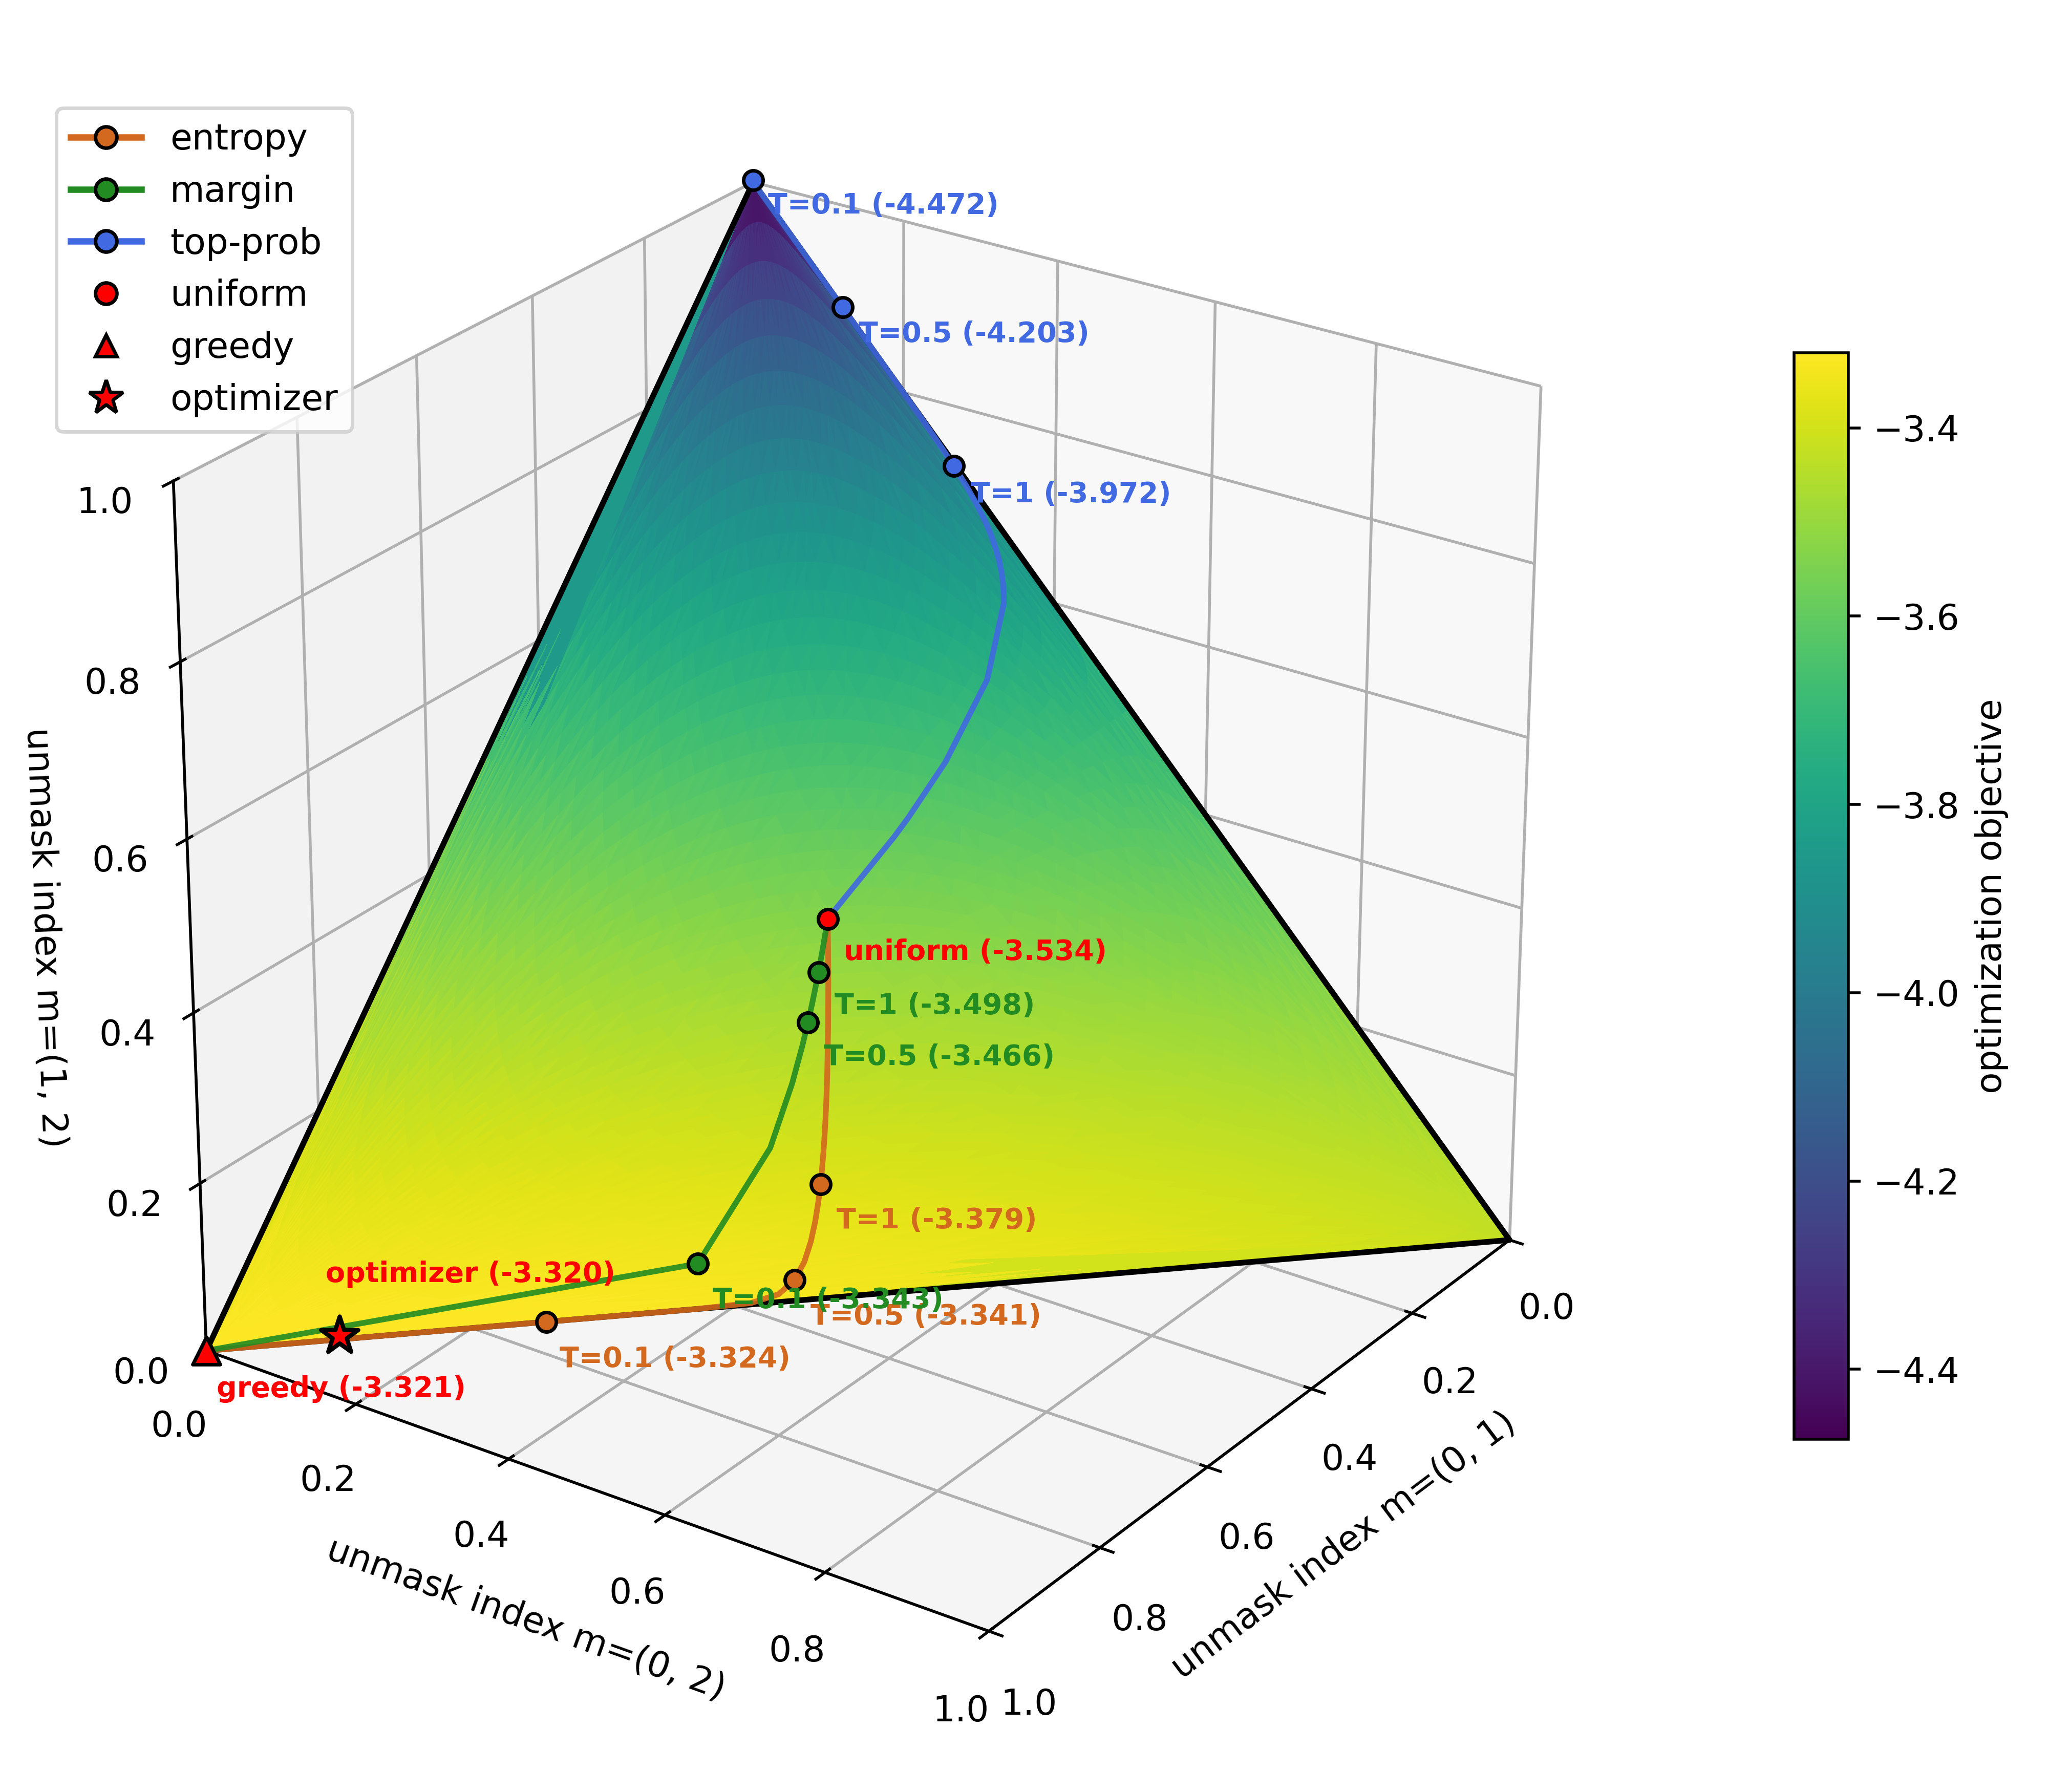
\includegraphics[height=0.17\textheight,width=\linewidth,keepaspectratio]{figs/policy_simplex.png}
        \end{minipage}
        \caption{Landscape on policy simplex.}
        \label{fig:opt-intro}
    \end{subfigure}
    \hfill
    \begin{subfigure}[t]{0.38\linewidth}
        \centering
        \begin{minipage}[c][0.17\textheight][c]{\linewidth}
            \centering
            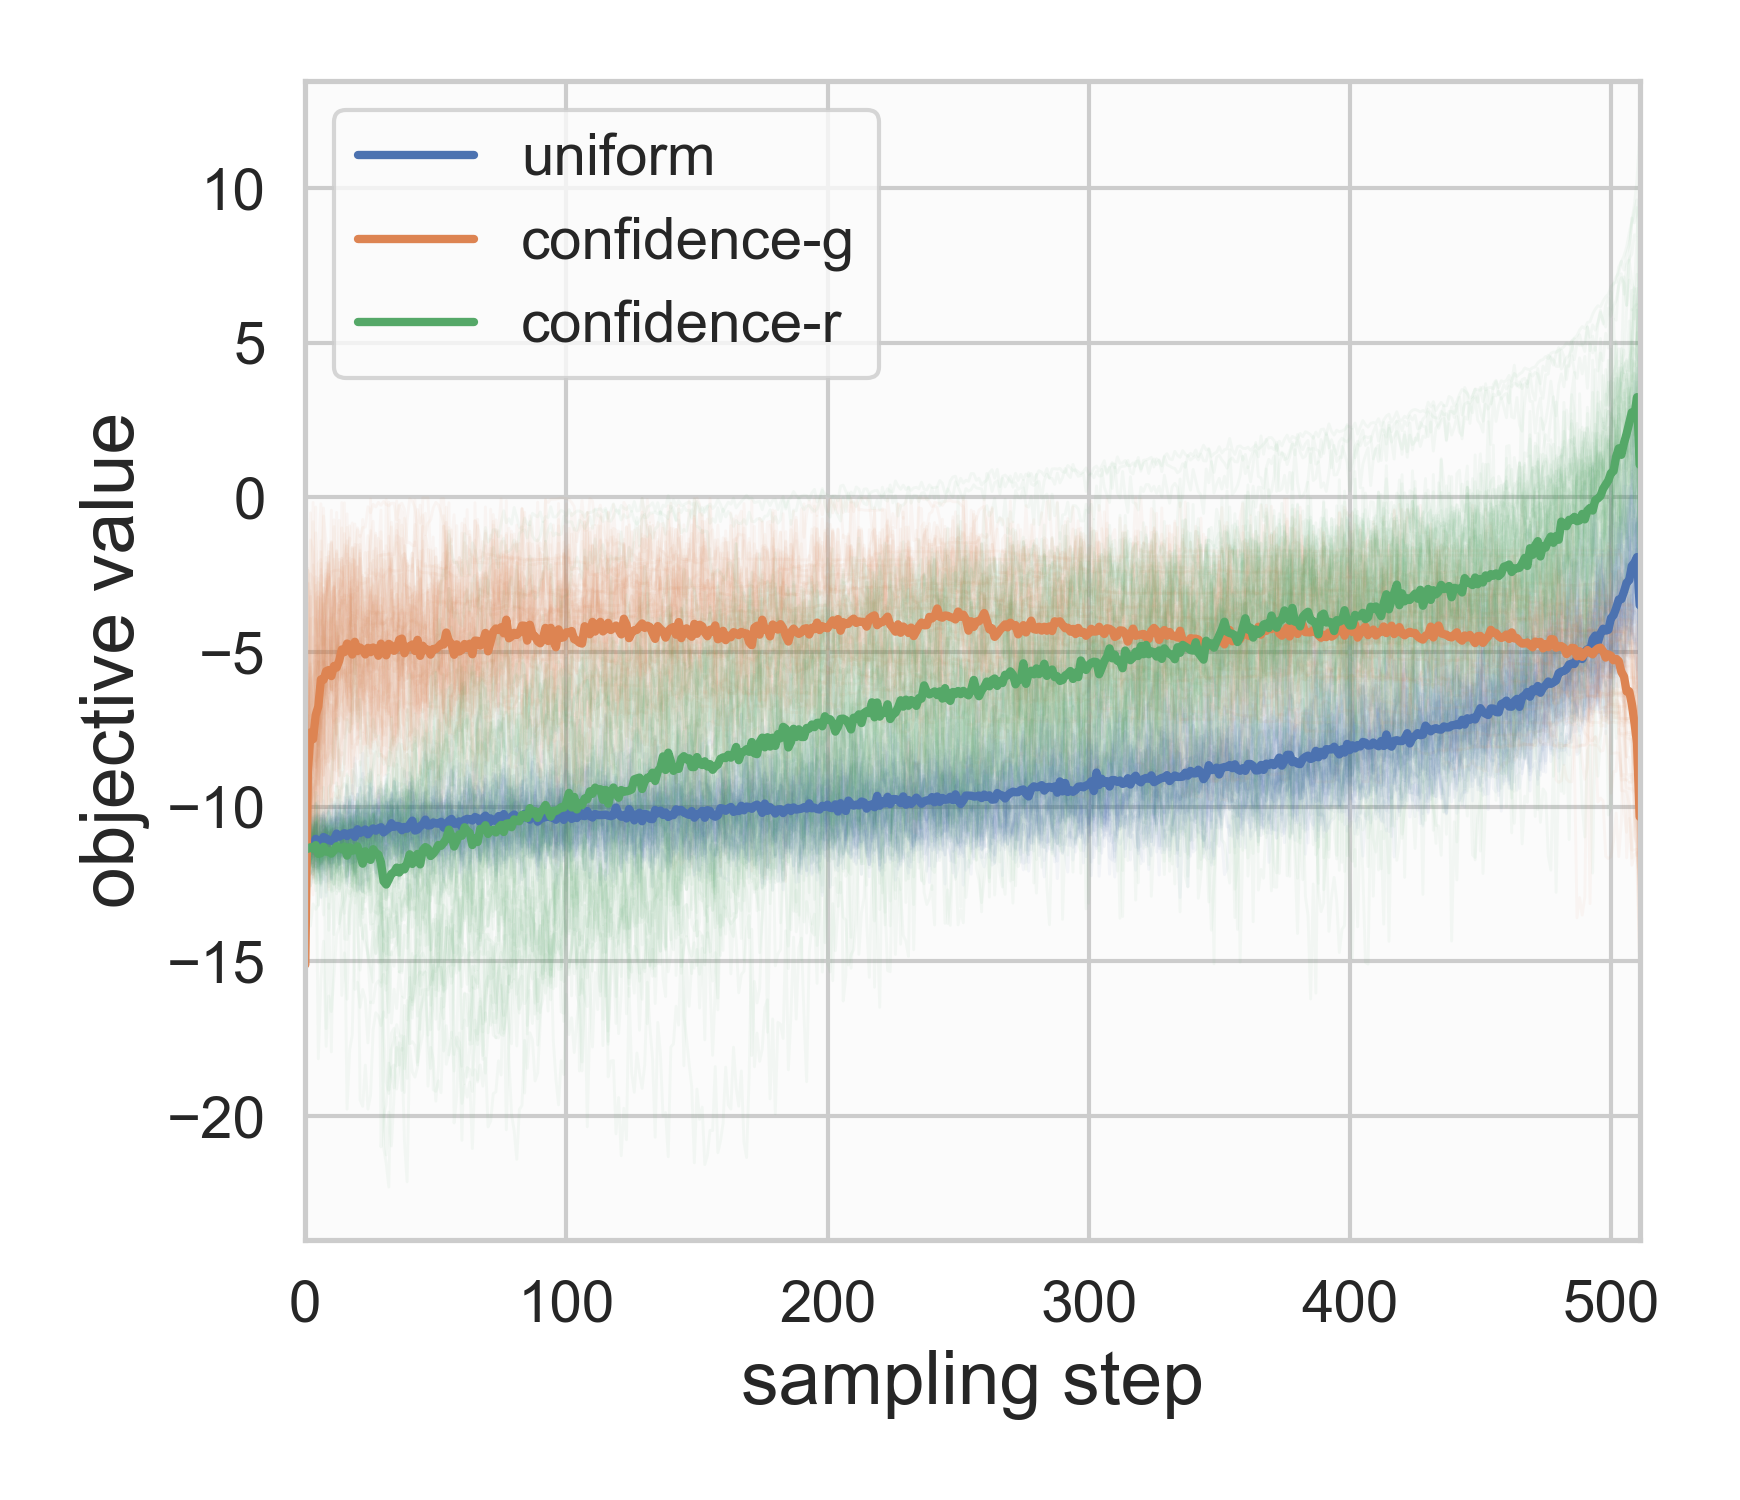
\includegraphics[height=0.17\textheight,width=\linewidth,keepaspectratio]{figs/objective_steps_512.png}
        \end{minipage}
        \caption{Likelihood objectives.}
        \label{fig:radd-obj-val}
    \end{subfigure}
    \hfill
    \begin{subfigure}[t]{0.3\linewidth}
        \centering
        \begin{minipage}[c][0.17\textheight][c]{\linewidth}
            \centering
            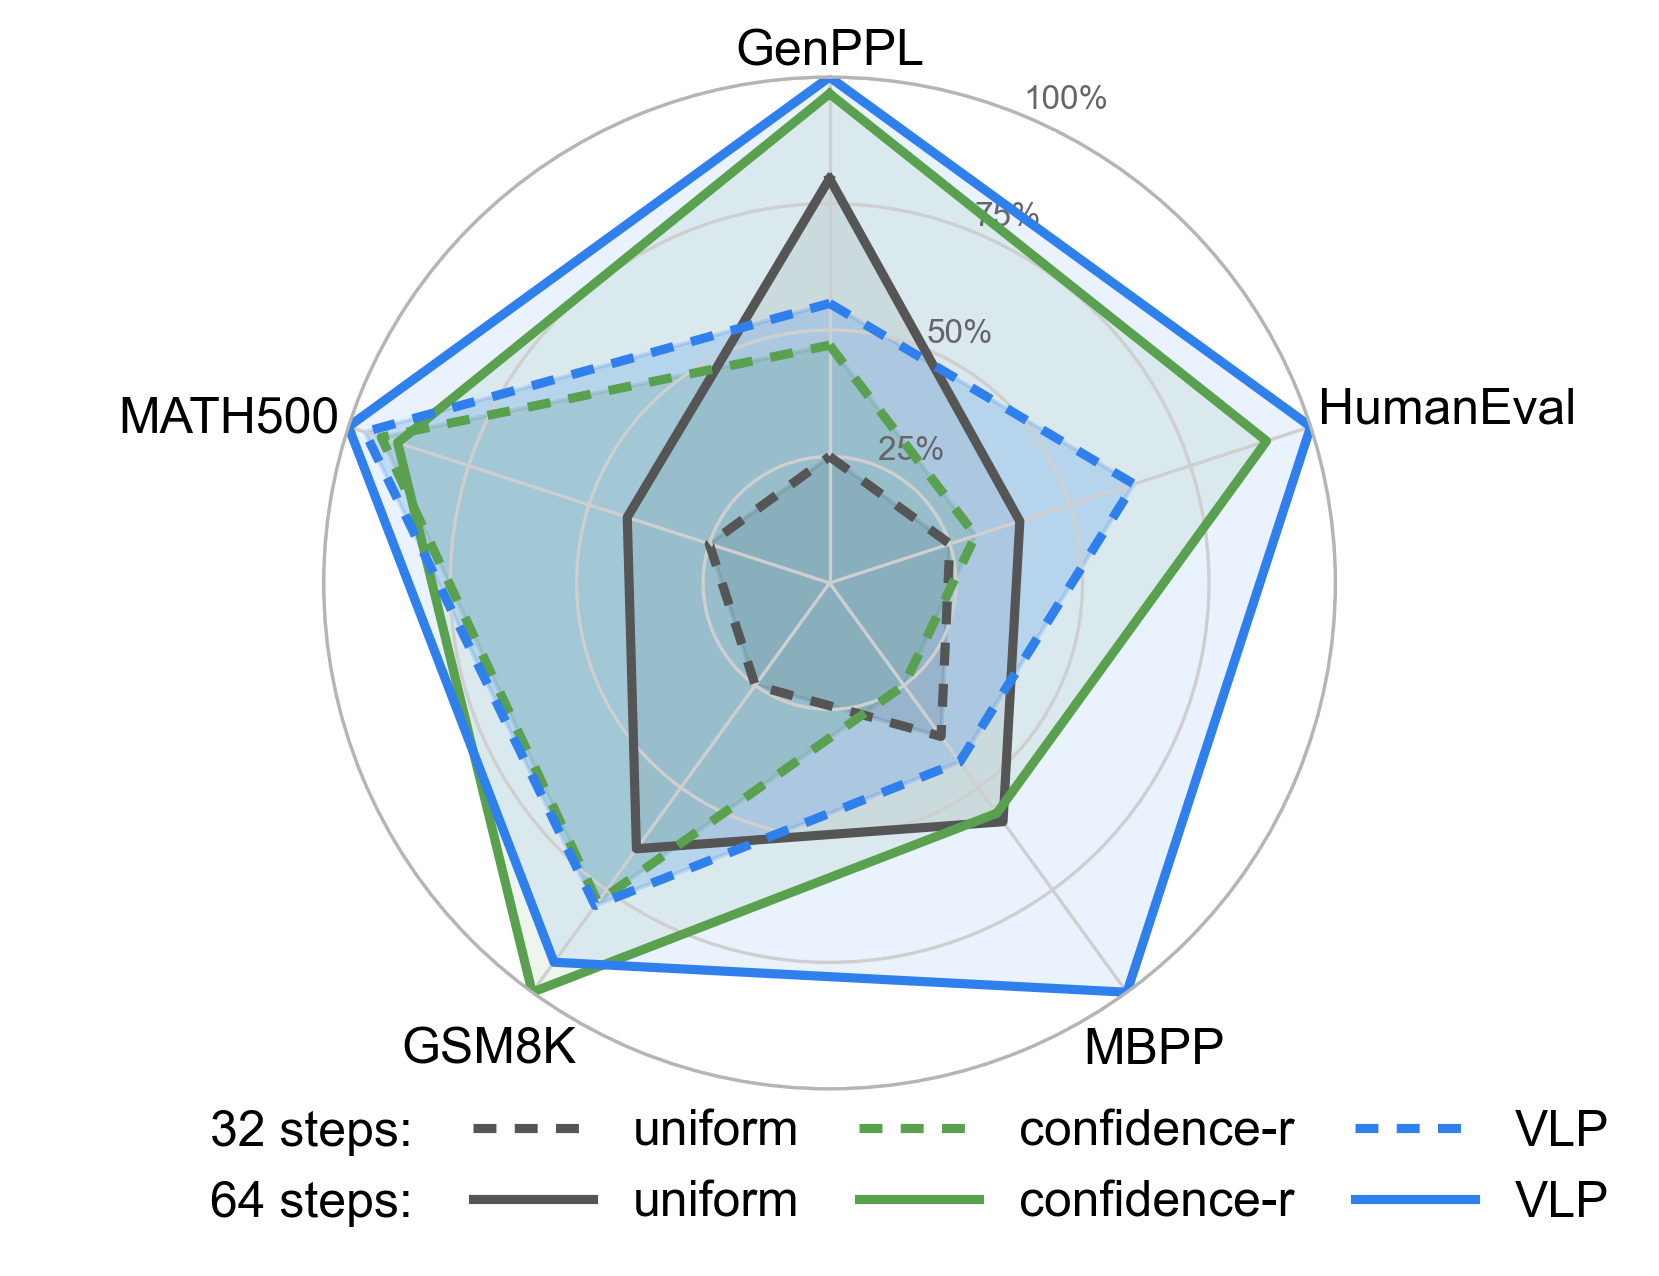
\includegraphics[height=0.17\textheight,width=\linewidth,keepaspectratio]{figs/radar_steps32_64.png}
        \end{minipage}
        \caption{VLP evaluation.}
        \label{fig:vlp-eval}
    \end{subfigure}
    \label{fig:optimality-exp}
    \caption{\textbf{(a)}: The landscape of the local likelihood maximization problem \eqref{eq:trainable_confidence} over the policy simplex, and different unmasking methods with their attained objective values. \textbf{(b)}: Monte Carlo estimation of per-step local objective values \eqref{eq:trainable_confidence} attained by different unmasking methods in text generation with RADD~\citep{ou2025absorbingdiscretediffusionsecretly}. \textbf{(c)}: Selected evaluation results (see Table~\ref{tab:text-gen} and~\ref{tab:dream-all} for full version) of our likelihood-trained policy, VLP, compared to uniform and confidence unmasking methods in RADD text generation, and Dream-7B~\citep{ye2025dream7bdiffusionlarge} code and math generation. Data are rescaled between the best and worst performance among the compared methods.}
\end{figure}

Diffusion language models \citep{li2022diffusion} recently emerged as a potential alternative to their autoregressive counterparts for language modeling with advances in discrete diffusion \citep{austin2021structured, lou2024discrete, sahoo2024simple, shi2024simplified, ou2024your}. These models conduct training and inference by leveraging a forward-backward pair of continuous-time Markov chains (CTMC) evolving over continuous time $t\in(0,1)$ in a discrete state space. In the forward (noising) process, a training data sample is gradually corrupted into pure noise; then the model aims to learn its reverse, i.e. the backward (denoising) process, that refines a random draw from pure noise step by step back to data.

The CTMCs become more specific when we focus on masked diffusion models (MDMs) \citep{shi2024simplified,sahoo2024simple}, currently one of the most representative discrete diffusion schemes for language modeling. In the forward process of MDMs, each token in the input sequence independently jumps to a special mask token \mask{} with the same probability, and stays in \mask{} thereafter. During inference, the backward process begins with an all-mask sequence and learns to perform random unmasking, converting each \mask{} to a predicted text token. In this way, compared to autoregressive models that maintain a left-to-right ordering, MDMs offer an enhanced flexibility in training and generation order.

Nonetheless, sampling from the backward process introduces several practical subtleties. For fast sampling, it is desirable to take large time steps $\Delta t$, unmasking multiple tokens per step. However, the ideal continuous-time process requires $\Delta t \to 0$ to guarantee simulation accuracy. Therefore, as unmasking can be conducted in arbitrary order, which token(s) should we choose to unmask?

Standard MDM training does not answer this question because it only learns a continuous-time transition rate, but several proposals exist. A first idea is to assign each token the same chance of being unmasked at each sampling step, known as $\tau$-leaping strategy \citep{campbell2022continuous} or \textit{uniform} unmasking. The motivation for this approach is that in the continuous-time limit, each token position has the same unmasking rate, symmetric to the forward process. However, this method 
%is not theoretically grounded because the uniform property no longer holds after discretization. As a result, it 
%\jiaxin{I believe the theoretical backward is indeed a uniform choice even under discretization.}
usually underperforms in empirical studies of MDM inference \citep{zhao2024informed}.

\begin{wrapfigure}{r}{0.45\textwidth}
    \vspace{-1em}
    \centering
    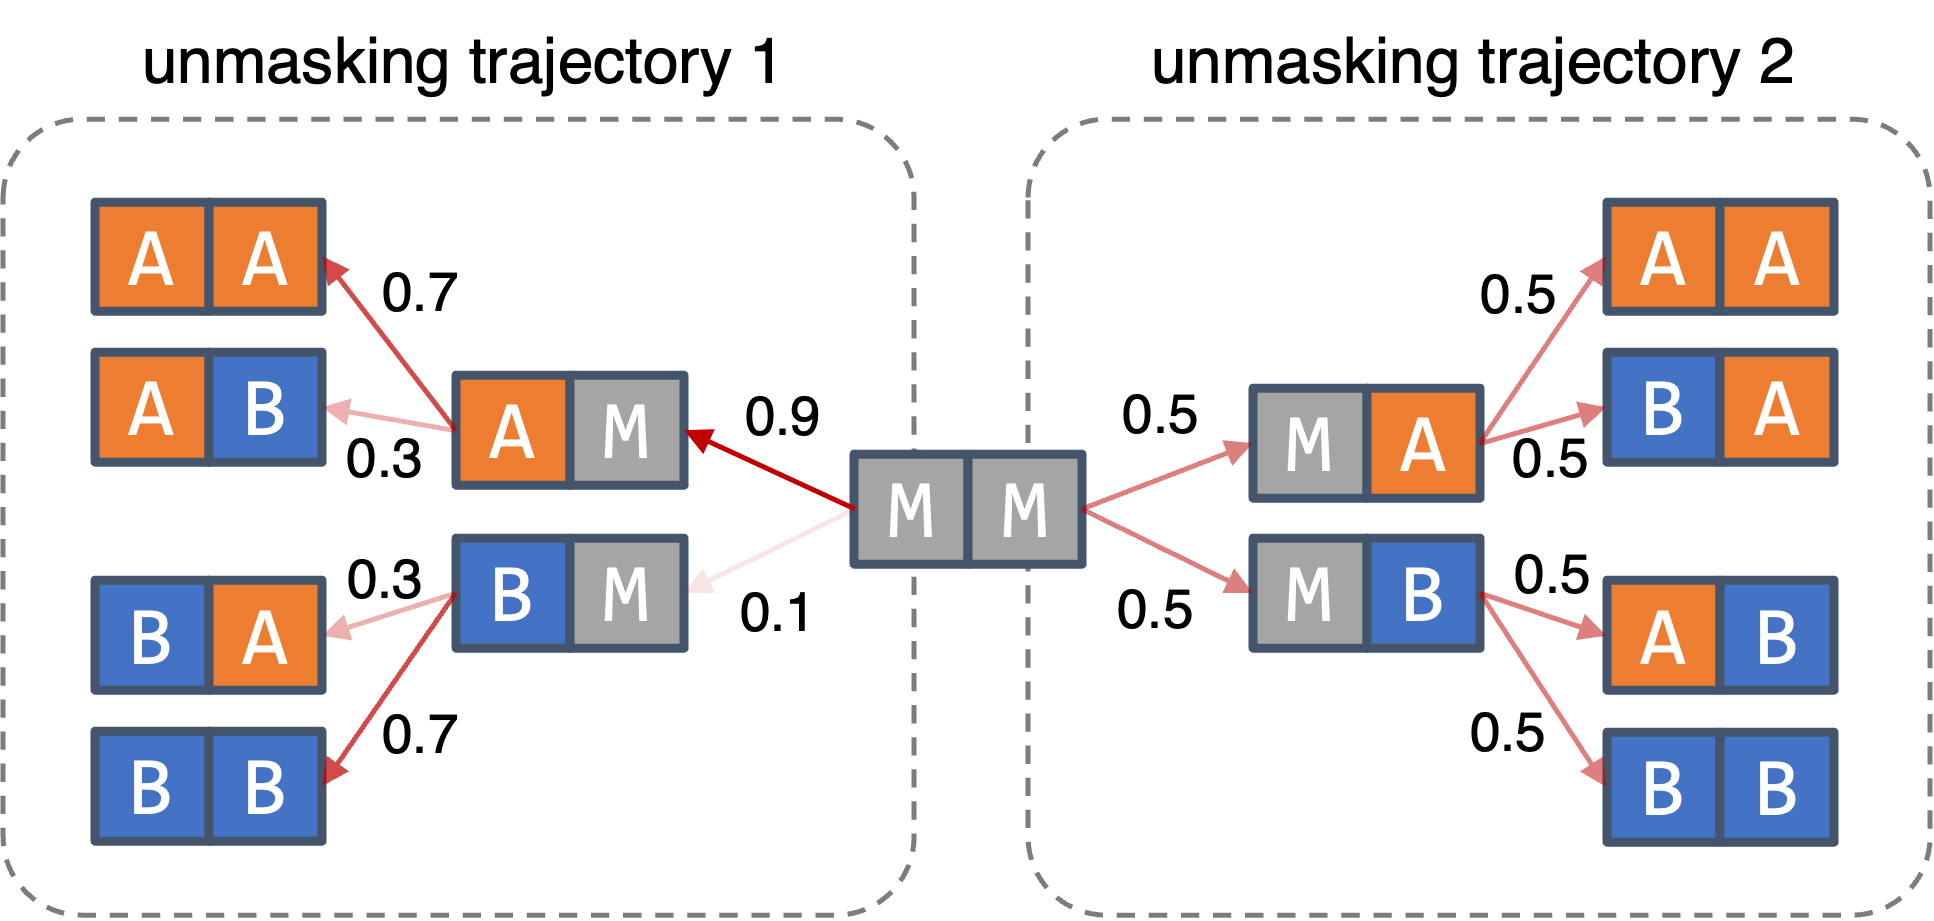
\includegraphics[width=0.98\linewidth]{figs/illustration-icml.png}
    \caption{Two different sampling trajectories of decoding a length-2 sequence on a simple vocabulary $\{\texttt{A},\texttt{B}\}$. Confidence-based unmasking indicates that trajectory 1 is preferred.}
    \label{fig:illustrate}
    \vspace{-1.5em}
\end{wrapfigure}

Another method that works better in practice is \textit{confidence}-based unmasking \citep{kim2025train,nie2025largelanguagediffusionmodels,ye2025dream7bdiffusionlarge}. Specifically, it prioritizes unmasking positions where the model is more confident in its vocabulary distribution. For example, in Figure~\ref{fig:illustrate}, the left masked token has prediction $p(\texttt{A})=0.9,p(\texttt{B})=0.1$, which shows the model's higher confidence than the right position with $p(\texttt{A})=p(\texttt{B})=0.5$, and hence gets unmasked first. Here, confidence can be quantified by various metrics such as negative entropy, top probability, and the margin between the top-2 probabilities; see details in Section~\ref{sec:prelim}.

\subsection{Theoretical Understanding of Confidence}

Despite its empirical success, the design of confidence-based methods remains largely heuristic and the reasons for their success are not fully clear. Although earlier work provides some intuition that these methods plan for a good reasoning path \citep{kim2025train}, there is still a lack of theoretical justification for their advantages over the uniform scheme. This is the first question we aim to address in this paper: \emph{Is confidence unmasking provably better for the time-discretized backward process?}

In the first half of this paper, we formulate an optimization problem of searching for the best unmasking policy $\pi$, that is, the random mapping from current sampling step to the index set for next unmasking step. The objective of the problem is to maximize the sampling log-likelihood $\log p_0^{\theta,\pi}$ with respect to the discrete-time policy $\pi$ and a parameterized backward process $p_t^\theta$ learned separately, i.e.
\begin{align}\label{eq:obj}
    \max_\pi \EE_{\bm x_0\sim q_0}\log p^{\theta,\pi}_0(\bm x_0),
\end{align}
where $q_0$ is the unknown source data distribution. We show that, under a data-agnostic approximation and a local restriction of objective for tractability, entropy-based confidence unmasking emerges as a (near-)optimal policy (Section~\ref{sec:confidence}). This indicates a provable advantage of confidence unmasking over other methods in terms of sample likelihood, consistent with empirical observations. We also conduct numerical evaluations in synthetic and real text generation tasks to support our theoretical claims on the near-optimality of confidence-based unmasking methods (Figure~\ref{fig:opt-intro},~\ref{fig:radd-obj-val}).

\subsection{Unmasking Policy via Likelihood Optimization}
On the other hand, the reductions in our theory also suggest that confidence unmasking is not optimal, as it does not maximize the original objective \eqref{eq:obj}. This motivates us to revisit \eqref{eq:obj} and ask a second question: \emph{Can we further develop advanced unmasking policies based on the original likelihood optimization problem?}

The second half of this paper is devoted to this extension from confidence to trainable policies. Specifically, we develop Variational Likelihood Policy (\alg{}), a prototypical training framework based on \eqref{eq:obj} with variational inference to optimize a neural-network-parameterized policy $\pi$, serving as an auxiliary trainable component to pretrained MDMs (Section~\ref{sec:method}). We train and evaluate \alg{} on differently scaled DLMs, including RADD~\citep{ou2025absorbingdiscretediffusionsecretly}, Dream-7B~\citep{ye2025dream7bdiffusionlarge}, and DiffuCoder-7B~\citep{gong2025diffucoderunderstandingimprovingmasked} across text, code, and math generation tasks (Figure~\ref{fig:vlp-eval}). The evaluation results indicate that our likelihood-trained policy, \alg{}, effectively learns unmasking policies and consistently matches or surpasses the performance of confidence-based methods across different models and tasks.

To summarize, in this paper, we propose a systematic framework based on likelihood optimization to analyze MDM unmasking methods. Our contribution lies in

\begin{itemize}[noitemsep, topsep=0pt]
    \item \textbf{Theoretical understanding of confidence:} We prove the theoretical advantages of confidence unmasking in terms of near-optimality in likelihood optimization (Section~\ref{sec:confidence}), supported by numerical analysis on the optimization objective in synthetic and real generation scenarios (Section~\ref{subsec:numerical-analysis}; Figure~\ref{fig:opt-intro},~\ref{fig:radd-obj-val}).

    \item \textbf{Principled design of trainable unmasking methods:} We design a likelihood-trained unmasking policy, \alg{} (Section~\ref{sec:method}), with variational inference and show its advantages through comprehensive evaluations across text, code, and math generation tasks on MDMs at different scales (Section~\ref{subsec:vlp-eval}; Figure~\ref{fig:vlp-eval}).

\end{itemize}
\section{Background}\label{sec:prelim}
\subsection{Masked Diffusion Models}
A continuous-time discrete diffusion model consists of a forward noising process and a backward denoising process, both continuous-time Markov chains. In the forward process, training samples are progressively corrupted into pure noise. The model learns the corresponding backward process that inverts this corruption, then generates new samples by running the backward process from noise.

\textbf{Continuous-time Markov chain.} We consider a discrete state space $\mathcal{X}$. A continuous-time Markov chain (CTMC) is a process $\vx_t$ on $\mathcal X$ with ${t \in [0, 1]}$, starting from an initial data distribution $q_0(\vx_0)$. A CTMC is characterized by a time-dependent transition rate matrix $Q_t \in \mathbb{R}^{|\mathcal{X}| \times |\mathcal{X}|}$. For distinct states $\vx_t, \vy \in \mathcal{X}$, $Q_t(\vx_t, \vy) \ge 0$ defines the instantaneous transition rate from $\vx_t$ to $\vy$, i.e., over an infinitesimal time interval $[t,t+\Delta t]$ the transition probability is given by
\begin{equation}\label{eq:infinitesimal_transition}
    q_{t+\Delta t|t}(\vy|\vx_t) = \delta(\vx_t, \vy) + Q_t(\vx_t, \vy) \Delta t + o(\Delta t),
\end{equation}
where $\delta$ is the Kronecker delta.
Equivalently, the marginal distribution $q_t\in\Delta(\mathcal X)$ evolves according to the Kolmogorov ODE $dq_t/dt = q_t Q_t$.
Note that the diagonal entries of $Q_t$ should satisfy $Q_t(\vx_t, \vx_t) = - \sum_{\vx_t \neq \vy} Q_t(\vx_t, \vy)$ to ensure that $q_t$ sums to $1$. 

\textbf{The masking and unmasking processes.} In the forward process of MDMs with law $q_t$, the transition rate matrix is commonly parameterized as $Q_t = \sigma(t)Q$, where $\sigma(t)$ is a scalar noise schedule and $Q$ is a constant rate matrix determined by the model design \citep{campbell2022continuous}. For MDMs, a specific $Q$ is adopted so that over an infinitesimal interval $[t,t+\Delta t]$, the token-level transition probabilities are
\begin{equation*}
    q_{t+\Delta t|t}(y|x)=
\begin{cases}
\sigma(t)\,\Delta t + o(\Delta t), & y=\mask,\\
1-\sigma(t)\,\Delta t - o(\Delta t), & y=x\in\mathcal V,\\
0, & \text{otherwise},
\end{cases}
\end{equation*}
with a state space $\mathcal V\cup\{\mask\}$. Letting $\bar\sigma(t)=\int_0^t\sigma(s)\,ds$, the distribution of a token at time $t$ conditioned on the initial state $x$ is given by
\begin{equation*}
\label{eq:forward_seq}
    q_{t|0}(y|x)
=
e^{-\bar\sigma(t)}\mathbf 1[y=x]
+
\bigl(1-e^{-\bar\sigma(t)}\bigr)\mathbf 1[y=\mask].
\end{equation*}
Due to token-wise independence, the forward process for a length-$L$ sequence is the product CTMC on $(\mathcal V\cup\{\mask\})^L$, with the joint distribution
\begin{equation*}
\label{eq:forward_distribution}
        q_{t|0}(\bm x_t|\bm x_0)=\prod_{i=1}^L q_{t|0}(x_t^i|x_0^i).
\end{equation*}

The model aims to learn the time-reversal of the forward process $q_t$, denoted by $p_t^\theta$: starting from an all-mask terminal state, we randomly unmask each position to a token in the vocabulary. We provide mathematical details in Appendix~\ref{sec:literature-appendix}.


\subsection{Related Works on MDM Inference}\label{subsec:confidence}

\textbf{Confidence-based unmasking.}
A common alternative to uniform unmasking in masked diffusion models (MDMs) is to prioritize positions where the model exhibits higher predictive confidence. Concretely, given the conditional token distribution
$p_i(v) = p_t^\theta(x_{t-\Delta t}^i = v \mid \bm x_t)$
at position $i$, a confidence score $c_i$ is computed and used to guide the unmasking order. Popular choices include:
\begin{itemize}[noitemsep, topsep=0pt]
    \item {Negative entropy} \citep{ye2025dream7bdiffusionlarge}, $c_i = \sum_v p_i(v)\log p_i(v)$;
    \item {Top-1 probability} \citep{nie2025scalingmaskeddiffusionmodels}, $c_i = \max_v p_i(v)$;
    \item {Top-2 margin} \citep{kim2025train}, $c_i = p_i(v_1) - p_i(v_2)$, where $v_1, v_2$ are the two most likely tokens at $i$.
\end{itemize}
Given these scores, unmasking strategies are typically either \emph{greedy}, selecting the top-$N$ positions with highest confidence, or \emph{randomized}, for example by perturbing confidence scores before top-$N$ selection \citep{kim2025train} or sampling positions proportionally via a softmax transformation \citep{ye2025dream7bdiffusionlarge}. While simple and effective in practice, these approaches are largely heuristic and do not arise from an explicit optimization objective. Beyond fixed-size selection, \citet{benhamu2025eb} propose an adaptive sampler that dynamically chooses both which and how many tokens to unmask, justified by a KL-based entropy bound on joint dependence error.

\textbf{Trainable inference methods.}
Beyond fixed heuristics, several works treat the unmasking order as a trainable policy. We defer these discussions to Appendix~\ref{sec:literature-appendix}. 

\iffalse
\textbf{Theoretical perspectives and limitations.}
Recent theoretical work has begun to clarify why inference strategies play a central role in discrete and masked diffusion models. Formalizations of discrete diffusion as continuous- or discrete-time Markov processes show that commonly used approximations, such as $\tau$-leaping, can introduce systematic bias that compounds in high-dimensional discrete spaces \citep{austin2021structured, campbell2022continuous}. From a Gibbs sampling perspective, diffusion inference can be viewed as a sequence of conditional updates, where the unmasking order acts as a scan rule that critically affects convergence and stability \citep{hayakawa2025demystifying, peng2025path}. 

These analyses also help explain the limitations of confidence-based heuristics. Greedy unmasking based on local confidence resembles coordinate descent in an implicit energy landscape, making it highly sensitive to early-stage errors that can propagate and trap the sampler in suboptimal regions \citep{kholkin2025sampling, chen2025beyond}. While learning-based approaches partially address these issues, they often optimize over local transitions or trajectories rather than globally optimal paths through the diffusion process.

\textbf{Our perspective.}
Building on these insights, we adopt a more foundational viewpoint: rather than treating confidence heuristics or learned policies as ad hoc design choices, we ask what inference objective they implicitly approximate. This perspective allows us to (i) derive confidence-based unmasking from a directly trainable global objective, and (ii) explain when and why such heuristics become suboptimal under certain data or model regimes.
\fi

\iffalse

\textbf{Confidence-based methods.} As an alternative to uniform unmasking, existing works propose to prioritize unmasking tokens where the MDM's prediction confidence is higher. In these methods, we first compute MDM's confidence $c_i$ at each token position $i$ using the predicted token probabilities $p_i(v)=p_t^\theta(x_{t-\Delta t}^{i}=v|\bm x_t)$. Common metrics of confidence include
\begin{itemize}[noitemsep, topsep=0pt]
    \item negative entropy \citep{ye2025dream7bdiffusionlarge}, where $c_i=\sum_v p_i(v)\log p_i(v)$;
    \item top-1 probability \citep{nie2025scalingmaskeddiffusionmodels}, where $c_i=\max_v p_i(v)$;
    \item top-2 probability margin \citep{kim2025train}, where $c_i=p_i(v_1)-p_i(v_2)$ and $v_1, v_2$ denotes the 2 tokens with highest probabilities among $\mathcal V$.
\end{itemize}
With the computed confidence, one can design a family of unmasking strategies that are either \textit{greedy}---directly select top-$N$ indices with the highest confidence to unmask, or \textit{randomized}---adding noise to the confidence score before top-$N$ \citep{kim2025train} or converting into unmasking probabilities by softmax function \citep{ye2025dream7bdiffusionlarge}.

\textbf{Trainable methods.} 

Several works consider the ordering policy as a separate trainable entity \citep{peng2025path,jazbec2025learning} or construct update rules that allow the backwards process to learn policies that are more globally optimal, such as updating coherent groups of variables that share semantic dependencies \citep{meshchaninov2025guided} or using informed corrective steps to modify unmasked tokens \citep{zhao2024informed}. However, one weakness of these works is the lack of generalizable training framework that would illustrate the specific training objective that an optimal policy should optimize.


\textbf{Theory and understanding.} 

However, confidence based methods have several problems. First, most empirical methods are purely heuristics without an explicit training objective \citep{kim2025train} or learn a policy through reinforcement learning \citep{jazbec2025learning}. Second, the obtained policies optimize over local paths rather than global paths, which can lead to early consistency errors that propagate downstream \citep{chen2025beyond, hayakawa2025demystifying}. Recent theoretical work has established that inference in discrete and masked diffusion models is fundamentally governed by the sampling policy rather than the denoiser alone. Formalizations of discrete diffusion as discrete-time or continuous-time Markov processes show that commonly used approximations such as $\tau$-leaping can accumulate bias in high-dimensional discrete spaces \citep{austin2021structured, campbell2022continuous}. Interpreting diffusion sampling as Gibbs-style updates further reveals that the update order functions as a scan rule, which critically affects convergence and stability, motivating structured or planned update schedules \cite{hayakawa2025demystifying, peng2025path}. Energy-based perspectives partially explain why greedy confidence-based unmasking behaves like coordinate descent and is sensitive to early-stage errors, which can propagate and trap the sampler in suboptimal regions \cite{kholkin2025sampling, chen2025beyond}. We build on these ideas through a more foundational approach to understand how confidence methods can be derived from a directly trainable objective and also explain the suboptimality seen in certain data regimes.
\fi

% \sijin{Old version: Several recent works focus on selecting good sampling trajectories and discourage bad ones. This is a vital part of Seed Diffusion \citep{song2025seeddiffusionlargescalediffusion}. There are many ways to learn the conditional unmasking probabilities of the backwards process. However, constructing a sampling policy given these conditional probabilities can be difficult. In the following sections, we produce a framework that both formalizes the optimization problem of producing an optimal policy and show how previous heuristics arise from simplifications of the objective function.}
\section{Unmasking Policy Optimization}\label{sec:theory}
\subsection{Time-Discretized Process by Unmasking Policy}
Let $L$ be the sequence length. Denote $[L]=\{1,2,...,L\}$, and $\Delta(\mathcal S)$ the space of probability distributions on a set $\mathcal S$. Let $K$ be a positive integer and $0=t_0<t_1<...<t_K=1$ form a partition of the interval $[0,1]$. For efficient sampling, we aim to design a discrete-time unmasking process that operates on these timesteps $\{t_k\}$ in place of the learned MDM's backward diffusion $p_t^\theta$.

This can be done by introducing an unmasking policy. Formally, an unmasking policy is a mapping $$\pi:(\mathcal V\cup\{\mask\})^L\to\Delta(\mathrm{Pow}([L]))$$ from a current sampling state to a probability distribution over the collection of all subsets of $[L]$. In practice, it is customary to further restrict the support of the output distribution to the collection of size-$N$ subsets, where $N=L/K$. When $L$ is not divisible by $K$, we set the size of the final step to the remainder of $L$ divided by $K$.

Given a policy $\pi$ and the continuous-time backward process $p_t^\theta$ of a trained MDM, we can build a discrete-time process $p^{\theta,\pi}_k$ as follows. At each step of $p^{\theta,\pi}_k$, given the current state $\bm x_k$, the policy $\pi$ samples an index set $\mathcal U_k\subset[L]$ with probability $\pi(\mathcal U_k|\bm x_k)$, corresponding to a subset of the masked positions in $\bm x_k$. Then, the MDM's prediction $p_{t_k}^\theta(\cdot|\bm x_k)$ at time $t_k$ is used to fill in the newly unmasked tokens at $\mathcal U_k$, and the state transitions to $\bm x_{k-1}$. The transition probability from $\bm x_k$ to $\bm x_{k-1}$ is given by
\begin{align}\label{eq:policy-decompose}
    &{p}^{\theta, \pi}_{k}(\bm x_{k-1}|\bm x_k)
    =\pi(\mathcal U_k|\,\bm x_k)p^\theta_{t_k}(\bm x_{k-1}|\bm x_k)
\end{align}
where
\begin{align*}
    p^\theta_{t_k}(\bm x_{k-1}|\bm x_k)=\prod_{i\in\mathcal U_k}p^\theta_{k}(x_{k-1}^i|\bm x_k),\quad\mathcal U_k=\{i:x_k^i=\mask\neq x_{k-1}^i\}.
\end{align*}
For the unmasking policy to be valid, we constrain the unmasking trajectories $\mathcal{U} = \{\mathcal U_1,...,\mathcal U_K\}$ produced by the policy to form a partition of the full index set:
\begin{align*}
    \bigcup_{k=1}^K\mathcal U_k=[L];\quad  \mathcal U_k\cap\mathcal U_{k'}=\varnothing.
\end{align*}
Both the uniform ($\tau$-leaping) and confidence-based unmasking methods discussed above can be recovered by $p_k^{\theta,\pi}$ with appropriate choices of $\pi$.

\subsection{Likelihood Optimization}
Recall that a major question motivating this work is how we can theoretically compare different unmasking methods and search for the best one. This is made possible by connecting our discrete-time sampling process $p_k^{\theta,\pi}$ to likelihood optimization, a fundamental objective of generative modeling. Specifically, since $p_k^{\theta,\pi}$ is intended to recover the data distribution at the endpoint $k=0$, its generative performance can be measured by the sample log-likelihood under the training data distribution $q_0$. Under this criterion, the optimal policy is obtained by
\begin{align}\label{eq:min-obj}
    \min_\pi-\EE_{\bm x_0\sim q_0}\log p_0^{\theta,\pi}(\bm x_0),
\end{align}
cf. \eqref{eq:obj}. This objective is the original MDM training objective with the data marginal $p_0^\theta$ replaced by the policy-induced marginal $p_0^{\theta,\pi}$; this connection motivates our formulation.

The endpoint probability $p_0^{\theta,\pi}(\bm x_0)$ relates to the earlier sampling steps by marginalization:
\begin{align*}
    p_0^{\theta,\pi}(\bm x_0)&=\sum_{\bm x_1,...,\bm x_K}p_0^{\theta,\pi}(\bm x_0,\bm x_1,...,\bm x_K)=\sum_{\bm x_1,...,\bm x_K}\prod_{k=1}^Kp_k^{\theta,\pi}(\bm x_{k-1}|\bm x_k).
\end{align*}
Since the trajectories $(\bm x_0,\bm x_1,...,\bm x_K)$ have nonzero probability only when each $\bm x_k$ is a masked outcome of $\bm x_{k-1}$, each such trajectory is fully determined by a sequence of unmasking sets $\mathcal U=(\mathcal U_1,...,\mathcal U_K)$ applied to $\bm x_K$. Thus equivalently,
\begin{align*}
    p_0^{\theta,\pi}(\bm x_0)=\sum_{\mathcal U_1,...,\mathcal U_K}\prod_{k=1}^Kp_k^{\theta,\pi}(\bm x_{k-1}|\bm x_k)=\sum_{\mathcal U_1,...,\mathcal U_K}\prod_{k=1}^K\pi(\mathcal U_k|\,\bm x_k)\prod_{i\in\mathcal U_k}p^\theta_{t_k}(x_{k-1}^i|\bm x_k),
\end{align*}
due to \eqref{eq:policy-decompose}. Note that for non-mask tokens it always holds that $x^i_{k-1}=x^i_0$.
Plugging this into \eqref{eq:min-obj}, we have the optimization problem
\begin{align}\label{eq:margin-obj}
    \min_\pi-\EE_{q_0}\log\sum_{\mathcal U_1,...,\mathcal U_K}\prod_{k=1}^K\pi(\mathcal U_k|\,\bm x_k)\prod_{i\in\mathcal U_k}p^\theta_{t_k}(x_{k-1}^i|\bm x_k).
\end{align}
Directly solving \eqref{eq:margin-obj} is intractable. The sum over $(\mathcal U_1, \ldots, \mathcal U_K)$ has $\prod_{k=1}^{K} \binom{L_k}{N}$ terms, where $L_k$ denotes the number of masked positions at step $k$. This count grows exponentially in $K$ (e.g., $L!/(N!)^K$ when $L = KN$), and the log-sum-product structure prevents factorization across timesteps. This obstacle is structurally analogous to exact MAP decoding in autoregressive models, where global optimization is similarly intractable and local approximations (greedy decoding, beam search) are standard~\citep{chen2025decodinggameminimaxoptimality}. In Sections~\ref{sec:confidence} and~\ref{sec:method} we develop two such approximations to \eqref{eq:margin-obj}: a single-step locality restriction that recovers confidence-based heuristics, and a variational lower bound that enables direct policy training. 

%\citet{turok2026duel} adopt a complementary tractability handle: by restricting to deterministic position selection, the trajectory marginalization collapses to a single term and yields exact likelihoods within this restricted class. Our framework instead approximates the original objective over the broader space of stochastic policies, which encompasses the randomized heuristics used in practice.


% Moreover, we assume that we have access to the global coefficients $w$ computed by transition probabilities of each global sampling path. To maximize this objective on each fixed $\bm x_0$, the optimal $\pi$ would assign all the probability weight to the sampling path with the highest total transition probability. This can recover confidence-based approach as a local greedy approximation to this optimal strategy.

% We finally need to optimize the expected objective with $\bm x_0\sim q_0$ (Figure~\ref{fig:placeholder}). As expectation preserves convexity, this is a convex optimization for $\pi$. Indexing each path with $i$, the problem is
% \begin{align*}
%     \min_{\pi}-\EE_{\bm x_0\sim q_0}\log\sum \pi_i w_i(\bm x_0),
% \end{align*}
% subject to the standard constraint that $\pi$ is a probability distribution. This resembles a logistic regression objective.

% We can characterize the optimal solution $\pi^*$. Introducing Lagrange multipliers $(\lambda_1,...\lambda_n, \mu)$, the Lagrangian is given by
% \begin{align*}
%     \mathcal L(\pi,\lambda,\mu)=-\EE_{\bm x_0\sim q_0}\log\sum \pi_i w_i(\bm x_0)-\sum\lambda_i\pi_i-\mu\left(\sum\pi_i-1\right).
% \end{align*}
% We have KKT conditions
% \begin{align*}
%     \nabla_i\mathcal L=-\EE_{\bm x_0\sim q_0}\left[\frac{w_i(\bm x_0)}{\sum \pi_i w_i(\bm x_0)}\right]-\lambda_i-\mu=0,\tag{stationarity}\\
%     \lambda_i\pi_i=0,\tag{complementary slackness}\\
%     \pi\in\Delta_n,\quad \lambda_i\geq0\tag{feasibility}
% \end{align*}
% For the sampling path indexed by $i$, define the path metric as
% $$f_i(\pi)=\EE_{\bm x_0\sim q_0}\left[\frac{w_i(\bm x_0)}{\sum \pi_i w_i(\bm x_0)}\right].$$
% Then, KKT condition suggests that $\pi^*$ satisfies $f_i(\pi^*)=f_j(\pi^*)$ for $i,j$ with $\pi_i,\pi_j>0$; and $f_i(\pi^*)> f_j(\pi^*)$ for $i,j$ with $\pi_i>0,\pi_j=0$. Basically, this means the optimal strategy $\pi^*$ will concentrate its weights on the sampling paths with highest path metric.

\section{Optimality of Confidence Heuristics}\label{sec:confidence}
\subsection{Locality Restriction}
The objective \eqref{eq:margin-obj} requires planning the entire unmasking trajectory $\mathcal U_1,\dots,\mathcal U_K$ globally, which is intractable. In this section, we instead minimize a local surrogate of \eqref{eq:margin-obj} at each step $k$:
\begin{align}
    \label{eq:oracle_confidence}
         \min_{\pi(\cdot|\bm x_k)} -\EE_{\bm x_0\sim q_0(\cdot|\bm x_k)}\log\sum_{\mathcal U_k} \pi(\mathcal U_k|\bm x_k) \prod_{i\in\mathcal U_k}p^\theta_{t_k}(x_{k-1}^i|\bm x_k).
\end{align}
Here, the expectation is taken over the conditional distribution $q_0(\cdot|\bm x_k)$, i.e.\ the distribution over clean data $\bm x_0$ that could produce $\bm x_k$ via the forward masking process. The notation $x^i_{k-1}$ denotes the value at position $i\in\mathcal U_k$ produced by the single-step unmasking from $\bm x_k$ to $\bm x_{k-1}$.

In this local problem, the summation is reduced to the index subsets $\mathcal U_k$, and instead of the full policy $\pi$ we only need to optimize the single conditional distribution $\pi(\cdot|\bm x_k)$ by assigning probabilities $\pi(\mathcal U_k|\bm x_k)$ to each candidate subset $\mathcal U_k$. This is a convex optimization problem --- by the concavity of $\log$ and the fact that expectation preserves convexity \citep{boyd2004convex} --- and is therefore much more tractable.


\iffalse
The oracle objective has several problems that make it difficult to train directly. First, we only have access to  $p^\theta_{t-\Delta t|t}$ for large timesteps $\Delta t$. Second, the naive logsum of the unmasked index set trajectories requires us to sum over an exponentially large number of possible trajectories. The natural fix to the first issue is to replace the $q$ with $p^\theta$ in the logsum:
\begin{equation}
    \begin{split}
        \min_\pi -\EE_{\bm x_0\sim q_0}\log \sum_{\substack{\mathcal U_1,...,\mathcal U_K}} \prod_{k=1}^{K} \pi(\mathcal U_{k}|\bm x_{k})\prod_{k=1}^{K} \prod_{i\in\mathcal U_{k}}p^\theta_{k-1|k}(\bm x^i_{k-1}|\bm x_{k})
    \end{split}
\end{equation}
In practice, we find that appropriately deep neural networks can learn very close approximations to $q$, and thus this assumption is quite natural. We can also easily approximate the expectation over $q_0$ with a simple average over the $x_0$ seen in the training.

In prior literature, to fix the second issue, we often introduce an evidence lower bound (ELBO). However, naively applying ELBO under our framework fails.

Instead of examining all the $k$ steps at once, suppose we find the optimal index set at each step, and build the policy trajectory step by step. More formally, we wish to find the policy $\pi$ such that for each $1 \leq k \leq  K$,


The idea here is that sampling the trajectories naively is computationally infeasible because the number of trajectories grows exponentially with $k$. Furthermore, in this formulation, we can replace $q_0$ with $q_0(\cdot | \bm x_k)$, where $q_0(\cdot | \bm x_k)$ is defined as the data distribution with the tokens in $\bm x_k$ being fixed. This replacement is possible because once we unmask a token, we do not change its value. Hence, at step $k$, the probability of $x_0$ having tokens on $U_{k+1}$ with values not corresponding to $x_k$ is zero. In practice, many likelihood functions are approximately convex, and thus building the trajectories through stepwise local optimizations may yield solutions close to the optimal policy. 
\fi

\subsection{Deriving Confidence Unmasking}
Another gap between heuristic unmasking strategies and our framework is that \eqref{eq:oracle_confidence} requires precise knowledge of the conditional data distribution $q_0$, while the heuristics are data-agnostic. When $q_0(\cdot|\bm x_k)$ is unknown, the natural (and only) approximation available is the MDM's own prediction at time $t_k$:
\begin{align}
    \label{eq:trainable_confidence}
         \min_{\pi(\cdot|\bm x_k)} -\EE_{\bm x_0\sim p^\theta_{t_k}(\cdot|\bm x_k)}\log\sum_{\mathcal U_k} \pi(\mathcal U_k|\bm x_k) \prod_{i\in\mathcal U_k}p^\theta_{t_k}(x_{k-1}^i|\bm x_k).
\end{align}

\subsubsection{Greedy Confidence Unmasking}
Define entropy at index $i$ to be
\begin{align*}
 H_k(i)=-\sum_{v\in\mathcal V} p^\theta_{t_k}(x^i_{k-1}=v|\bm x_k)\log p^\theta_{t_k}(x^i_{k-1}=v|\bm x_k).
\end{align*}
We have the following result on the optimality of greedy confidence unmasking based on negative entropy (cf.~Section~\ref{subsec:confidence}).

\begin{theorem}
    \label{thm:confidence}
     Consider a policy $\pi$ that selects an index set of size at least $N$. 
     If (1) $\pi$ is a deterministic policy, or (2) $p_{t_k}^\theta$ satisfies
     \begin{align*}
         \EE_{x^i\sim p_{t_k}^\theta(\cdot|\bm x_k)}\left[\frac{\prod_{i\in\mathcal U'}p_{t_k}^\theta(x^i|\bm x_k)}{\prod_{i\in\mathcal U}p_{t_k}^\theta(x^i|\bm x_k)}\right]\leq 1
     \end{align*}
     for some $\mathcal U$ and arbitrary $\mathcal U'$, then the optimal strategy $\pi^*$ to \eqref{eq:trainable_confidence} satisfies $\pi^*(\cdot|\bm x_k)=\mathbf1_{\mathcal U^*}$, where
     $$\mathcal U^*={\arg\max}_{|\mathcal U|=N}\sum_{i\in\mathcal U}-H_k(i).$$
\end{theorem}

In words, $\pi^*$ will deterministically output the index set $\mathcal U^*$ with the smallest total entropy (highest confidence) for the next step's unmasking. The proof is deferred to Appendix~\ref{subsec:proof-confidence}. We also leave remarks on the connection to prior entropy-based criteria and extensions to constrained confidence samplers in Appendix~\ref{subsec:proof-confidence}.

\iffalse
\begin{theorem}
     Assuming independence of tokens and that $q_0$ can be approximated by $p^\theta_{k-1|k}$, equation \ref{eq:trainable_confidence} will recover the policy associated with the \textbf{top-$N$ confidence strategy}.
     \begin{equation}
         \label{eq:}
         \min_\pi -\EE_{\bm x_0\sim p^\theta_{k-1|k}(\cdot|\bm x_k)}\log\sum_{\mathcal U_k} \pi(\mathcal U_k|\bm x_k) \prod_{i\in\mathcal U_{k}}p^\theta_{k-1|k}(\bm x^i_{k-1}|\bm x_k)
     \end{equation}
\end{theorem}
\fi

\subsubsection{Randomized Confidence Unmasking}
In Theorem~\ref{thm:confidence}, the optimality of the greedy confidence policy relies on one of two specific conditions. In the more general case where neither condition holds, greedy confidence can be suboptimal and the optimal $\pi^*$ becomes randomized. Nonetheless, in Theorem~\ref{thm:confidence-rand} we show that the optimal $\pi^*$ can be characterized as a perturbation of the greedy point $\mathbf 1_{\mathcal U^*}$. This resembles the randomized confidence unmasking used in practice (cf. Section~\ref{subsec:confidence}), offering theoretical support for its empirical effectiveness.

\begin{theorem}\label{thm:confidence-rand}
    Let $\pi^*(\cdot|\bm x_k)$ be the optimal policy to \eqref{eq:trainable_confidence}, and $\mathcal U^*$ as defined in Theorem~\ref{thm:confidence}. Let $\bm M_k$ be the second moment matrix of the random variables $\prod_{i\in\mathcal U}p^\theta_{t_k}(x^i|\bm x_k)$, with $\mathcal U$ enumerating over the index subsets. Then,
    \begin{align*}
        \pi^*(\mathcal U^*|\bm x_k)\geq 1-\lambda_{\max}(\bm M_k^{-1})\nm{\bm P\bm g_k}
    \end{align*}
    where $\bm g_k$ is a vector indexed by $\mathcal U$ with
    \begin{align*}
        g_k^{\mathcal U}=\EE_{\bm x_0\sim p^\theta_{k-1|k}}\left[\frac{\prod_{i\in\mathcal U}p^\theta_{t_k}(x^i|\bm x_k)}{\prod_{i\in\mathcal U^*}p^\theta_{t_k}(x^i|\bm x_k)}\right],
    \end{align*}
    and $\bm P$ is the projection to the hyperplane orthogonal to the all-one vector.
\end{theorem}

In words, while $\pi^*$ is not greedy, it still assigns a high probability to the top-confidence subset $\mathcal U^*$ if the predicted distribution $p^\theta_{t_k}$ is well-conditioned. We defer the proof to Appendix~\ref{subsec:proof-random}.

\subsubsection{Controlling Sub-Optimality Gap under Distribution Shift}
Note that our optimality results from \eqref{eq:trainable_confidence} involve a distribution shift from $q_0(\cdot|\bm x_k)$ to $p^\theta_{t_k}(\cdot|\bm x_k)$, and so an optimal policy for \eqref{eq:trainable_confidence} is suboptimal for \eqref{eq:oracle_confidence}. The following theorem bounds the suboptimality gap in terms of the difference between the two distributions.

\begin{theorem}
\label{thm:confidence_bounds}
    Suppose that the Renyi divergence between ${p}^\theta_{t_k}(\cdot|\bm x_k)$ and $q_0(\cdot |\bm x_k)$ for $\alpha = \infty$ is bounded in both directions by $\epsilon$ with $\epsilon \le 1$, i.e.
\begin{align*}
    D_\infty(q_0(\cdot |\bm x_k)\Vert p^\theta_{t_k}(\cdot | \bm x_k)) := \log \sup_{\bm x} \frac{q_0(\bm x|\bm x_k)}{{p}^\theta_{t_k}(\bm x|\bm x_k)} \leq \epsilon;\quad 
    D_\infty(p^\theta_{t_k}(\cdot | \bm x_k)\Vert q_0(\cdot |\bm x_k)) \leq \epsilon.
\end{align*}
Then, the ratio between the optimal value of \eqref{eq:trainable_confidence} and \eqref{eq:oracle_confidence} is bounded by $1+8\epsilon$.
\end{theorem}


\iffalse
\subsection{ELBO}
\begin{proposition}
\label{prop:naive_elbo}
    Naively using ELBO eliminates all signal for training policy.
\end{proposition}

The intuition here is that constructing an ELBO utilizes Jensen's inequality to switch the logsum to a sum of logs, but in this case, the operation disentangles the dependency between the policy $\pi$ and $p^\theta$. Thus, the naive ELBO will select a policy that is uniformly sampling tokens at random, which, as remarked before, does not perform well in practice.
\fi

% In practice, such as in \cite{kim2025train}, confidence policies are obtained through a randomized process where the top $M> N$ tokens are unmasked, their confidence scores are perturbed by samples $\epsilon$ of a noise distribution, and $M-N$ token of lowest perturbed confidence are remasked. This noising of the scores prevents the policies from strictly learning locally optimal trajectories. However, these learned policies will still be suboptimal to the oracle optimal policy, although possibly better than the deterministic top-$N$ confidence policy. Intuitively, the ability for the training to learn closer to the oracle optimal will heavily depend on the dynamics of the order statistics of the $\epsilon$ noise, and tuning such a hyperparameter can be nontrivial.

% Another approach, the one we will explore more carefully, is to obtain an ELBO-esque bound by viewing the trajectories as generated by some learnable distribution and constructing a bound through Jensen's inequality. The benefits of this final bound is that it aligns the closest to the original oracle objective, and in the following experiments, we show that it has improvements over prior known heuristics.

% \begin{proposition}
%     The following trainable bound is a lower bound on the oracle objective:
%     \begin{equation}
%         \begin{split}
%             &\min_\pi -\EE_{\bm x_0\sim q_0}\sum_{\substack{\mathcal U_1,...,\mathcal U_K}}r(\mathcal U_1,...,\mathcal U_K)\\
%             &\quad \log  \prod_{k=1}^{K} \pi(\mathcal U_{k}|\bm x_{k})\prod_{k=1}^{K} \prod_{i\in\mathcal U_{k}}{p}(\bm x^i_{k-1}|\bm x_{k})
%         \end{split}
%     \end{equation}
%     where $r(\mathcal U_1,...,\mathcal U_K)$ is the probability that a particular trajectory is sampled under a multinomial distribution. 
% \end{proposition}

% \begin{proposition}
% \label{prop:training}
% For any distribution $r(T\mid x_0)$ over trajectories $T=(U_1,\dots,U_K)$
% (possibly depending on $x_0$ but not on $\pi$), define
% \begin{equation}
% \begin{split}
% A_\pi(T)
% &:= \prod_{k=1}^K \pi(U_k \mid x_k)
%     \prod_{k=1}^K \prod_{i \in U_k} \hat p(x^{\,i}_{k-1} \mid x_k).
% \end{split}
% \end{equation}
% Then
% \begin{equation}
% \begin{split}
% &\mathbb E_{x_0 \sim q_0}
% \log \sum_T A_\pi(T)
% \;\\
% &\ge\;
% \mathbb E_{x_0 \sim q_0}\,
% \mathbb E_{T \sim r(\cdot\mid x_0)}
% \Big[
% \log A_\pi(T) - \log r(T\mid x_0)
% \Big].
% \end{split}
% \end{equation}
% \end{proposition}



% \iffalse
% Observation: If we have $s_\theta$ fixed and want to find best $\pi$ that minimizes $\mathcal L_k$, then intuitively $\pi$ will assign more weight to index sets where $s_\theta(t_{k+1},\bm x_{k+1})_{i,\mathcal V}$ has more imbalanced values (lower entropy)? Related to confidence-based policy.

% As a simple example, let us constrain that $\pi$ only draws singleton $\mathcal U$. What is going to be the optimal $\pi$? At index $i$, for $v\in\mathcal V$, denote $q^i_v$ to be the data token distribution and $s^i_v$ to be the predicted score. The objective becomes $-\EE_{i\sim\pi} \sum q_v^i\log s_v^i$. If we assume that $\sum s_v^i=S$ for all $i$ and $q_v^i=s_v^i/S$ (which is true for real score), then the objective becomes $-\EE_{i\sim\pi}H(s^i/S)$, where $H$ is the entropy. So the optimal strategy will be choosing the $i$ with the maximum entropy of its normalized score $s^i/S$. Typically, a high entropy distribution means the top score stands out, connected to the heuristic notation of confidence.
% \fi
% It turns out that we can derive confidence sampling as an optimal strategy in a simplified framework, after applying the following reductions.



% \textbf{Reduction 1: Local proxy.} At given $k$ and an intermediate sampling step $\bm x_k$, we greedily decide $\pi(\mathcal U_k|\bm x_k)$ by computing
% \begin{align*}
%     \min_\pi -\EE_{\bm x_0\sim q_0(\cdot|\bm x_k)}\log\sum_{\mathcal U_k} \pi(\mathcal U_k|\bm x_k) \prod_{i\in\mathcal U_{k}}p^\theta_{k-1|k}(\bm x^i_{k-1}|\bm x_k)
% \end{align*}
% % Here, $\bm x_0\succ \bm x_k$ means that the non-mask part of $\bm x_k$ shares the same tokens with $\bm x_0$, i.e. $\bm x_k$ is a possible masking outcome of $\bm x_0$.

% \textbf{Remark:} Since the forward process is defined as a CTMC that either keeps the token the same or masks it as an absorbing state, the optimal backwards policy should not reassign unmasked tokens in previous steps to other elements in the vocabulary. Therefore, optimizing over the conditional data distribution $q_0(\cdot | \bm x_k)$ gives us the same optimal policy as the marginal.
% % (Can we justify this approximation is fair? We can let every token have a probability that ranges from infinitesimally small, but nonzero, to 1. Anything that requires some probability to be zero will simply be bounded above by some epsilon.) 

\section{Building Trainable Unmasking Policy with Likelihood Principles}\label{sec:method}
Our discussions above not only justify confidence unmasking as a reasonable approach for generating credible samples by minimizing \eqref{eq:trainable_confidence}, but also suggest room for developing other strategies by directly optimizing \eqref{eq:obj}. This section presents \alg{}, a training and inference framework that learns a policy from \eqref{eq:obj} via variational inference. Notably, \citet{benhamu2025eb} explicitly suggest learning a parameterized adaptive sampler optimizing a KL-based bound as a direction for future work; \alg{} realizes this idea within our likelihood-maximization formulation (cf.~\eqref{eq:vlp}).

Recall that the log-likelihood in \eqref{eq:obj} can be expanded as
\begin{align*}
    \log p_0^{\theta,\pi}(\bm x_0) = \log\sum_{\mathcal U} p_0^{\theta,\pi}(\bm x_0, \bm x_1, ..., \bm x_K)
\end{align*}
by marginalization, where as in Section~\ref{sec:theory}, the intermediate states $\bm x_1, ..., \bm x_K$ are determined by the trajectory $\mathcal U=(\mathcal U_1, ..., \mathcal U_K)$ and the data point $\bm x_0$ through the unmasking process. Training directly from this log-likelihood is intractable due to the exponential summation over $\mathcal U$.

Instead, similar to \citep{wang2025learningorder}, we introduce a variant of the evidence lower bound (ELBO) of the log-likelihood. Let $w(\cdot|\bm x_0)$ be an arbitrary discrete probability distribution over trajectories, with $w(\mathcal U|\bm x_0)$ denoting the probability of $\mathcal U$. By Jensen's inequality,
\begin{align}
    \log p_0^{\theta,\pi}(\bm x_0) 
    = \log \EE_{\mathcal U \sim w(\cdot|\bm x_0)}\frac{p_0^{\theta,\pi}(\bm x_0, \bm x_1, ..., \bm x_K)}{w(\mathcal U|\bm x_0)}
    \geq \EE_{\mathcal U \sim w(\cdot|\bm x_0)}\log\frac{p_0^{\theta,\pi}(\bm x_0, \bm x_1, ..., \bm x_K)}{w(\mathcal U|\bm x_0)}.\label{eq:vlp}
\end{align}
Maximizing this lower bound aligns the auxiliary trajectory distribution $w(\cdot|\bm x_0)$ with the model's joint distribution $p_0^{\theta,\pi}(\bm x_0,\cdot)$, viewed as a measure over trajectories. Different choices of $w$ yield different gaps between the bound and the exact log-likelihood.

To discourage the parameterized distributions from collapsing to degenerate solutions, following standard practice in policy-based reinforcement learning \citep{schulman2017proximal}, we additionally introduce KL regularization between $\pi_\phi$ and a reference policy $\pi_\text{ref}$, and between $w_\phi$ and a reference $w_\text{ref}$, where $\pi_\text{ref}$ implements confidence unmasking and $w_\text{ref}$ is the uniform distribution over trajectories.

In \alg{}, both $w$ and $\pi$ are parameterized by neural networks $w_\phi$ and $\pi_\phi$ sharing weights $\phi$; see Section~\ref{subsec:architecture}. Substituting the parameterization into \eqref{eq:vlp}, the loss function we use for training VLP is
\begin{align*}
    \mathcal L(\phi) &:= -\EE_{\bm x_0\sim q_0}\, \EE_{\mathcal U\sim w_\phi(\cdot|\bm x_0)}\log\frac{p_0^{\theta,\pi_\phi}(\bm x_0, \bm x_1, ..., \bm x_K)}{w_\phi(\mathcal U|\bm x_0)} + \lambda\, \mathcal R(\phi),\\
    \mathcal R(\phi) &:= \mathrm{KL}(\pi_\phi\|\pi_\text{ref}) + \mathrm{KL}(w_\phi\|w_\text{ref}).
\end{align*}

We defer the detailed description of the model architecture and training/inference algorithms used in VLP to Appendix~\ref{sec:further-vlp}. 
\section{Experiments}\label{sec:exp}
In this section, we conduct two sets of experiments. In the first part, we provide empirical support for our optimality theory in Section~\ref{sec:confidence} by evaluating the local likelihood optimization objective \eqref{eq:trainable_confidence} attained by different unmasking strategies in synthetic and real text generation tasks. In the second part, we train unmasking policies with \alg{} and evaluate the resulting sampling performance on text, code, and math benchmarks across multiple masked diffusion models (MDMs). In addition to the main comparisons with uniform and confidence-based unmasking, we also study the effect of KL regularization, temperature, and the per-step unmasking schedule.

\subsection{Numerical Analysis on Likelihood Optimization}

\begin{figure}[h]
    \centering
    \begin{subfigure}[h]{0.4\linewidth}
        \centering
        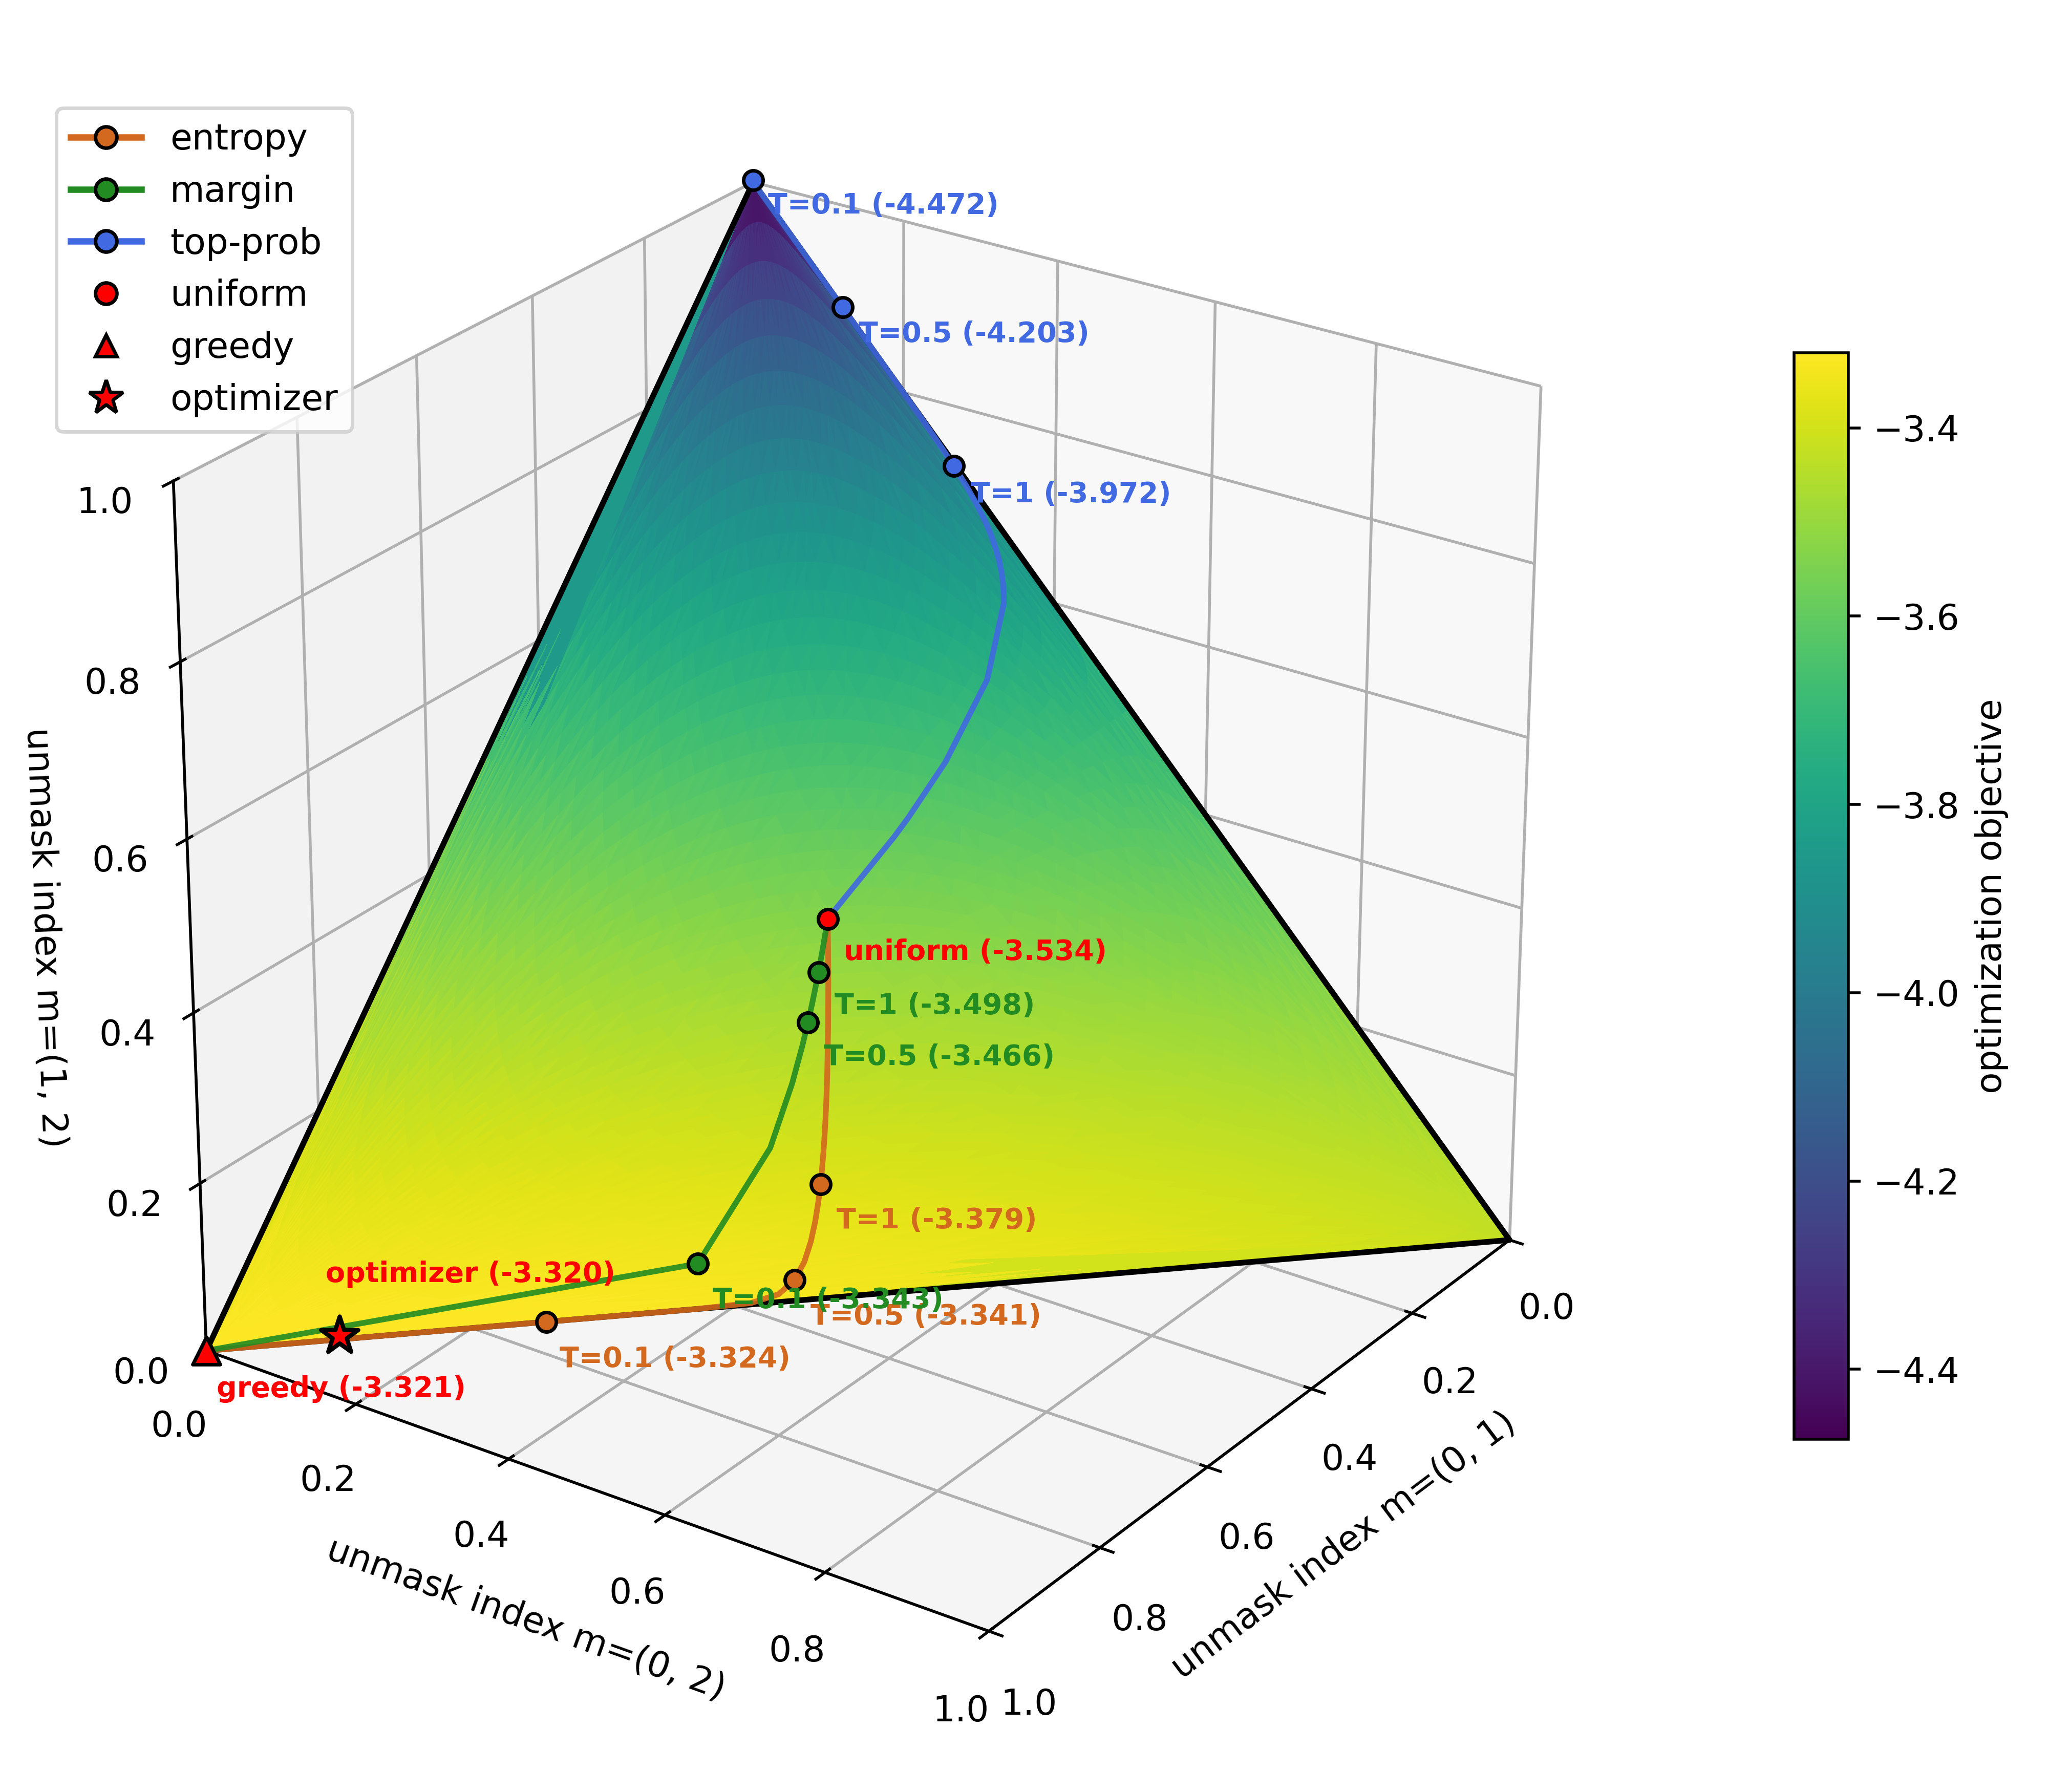
\includegraphics[width=\linewidth]{figs/policy_simplex.png}
        \vspace{-5pt}
        \caption{Landscape on the policy simplex.}
        \label{fig:opt-intro}
    \end{subfigure}
    \hfill
    \begin{subfigure}[h]{0.58\linewidth}
        \centering
        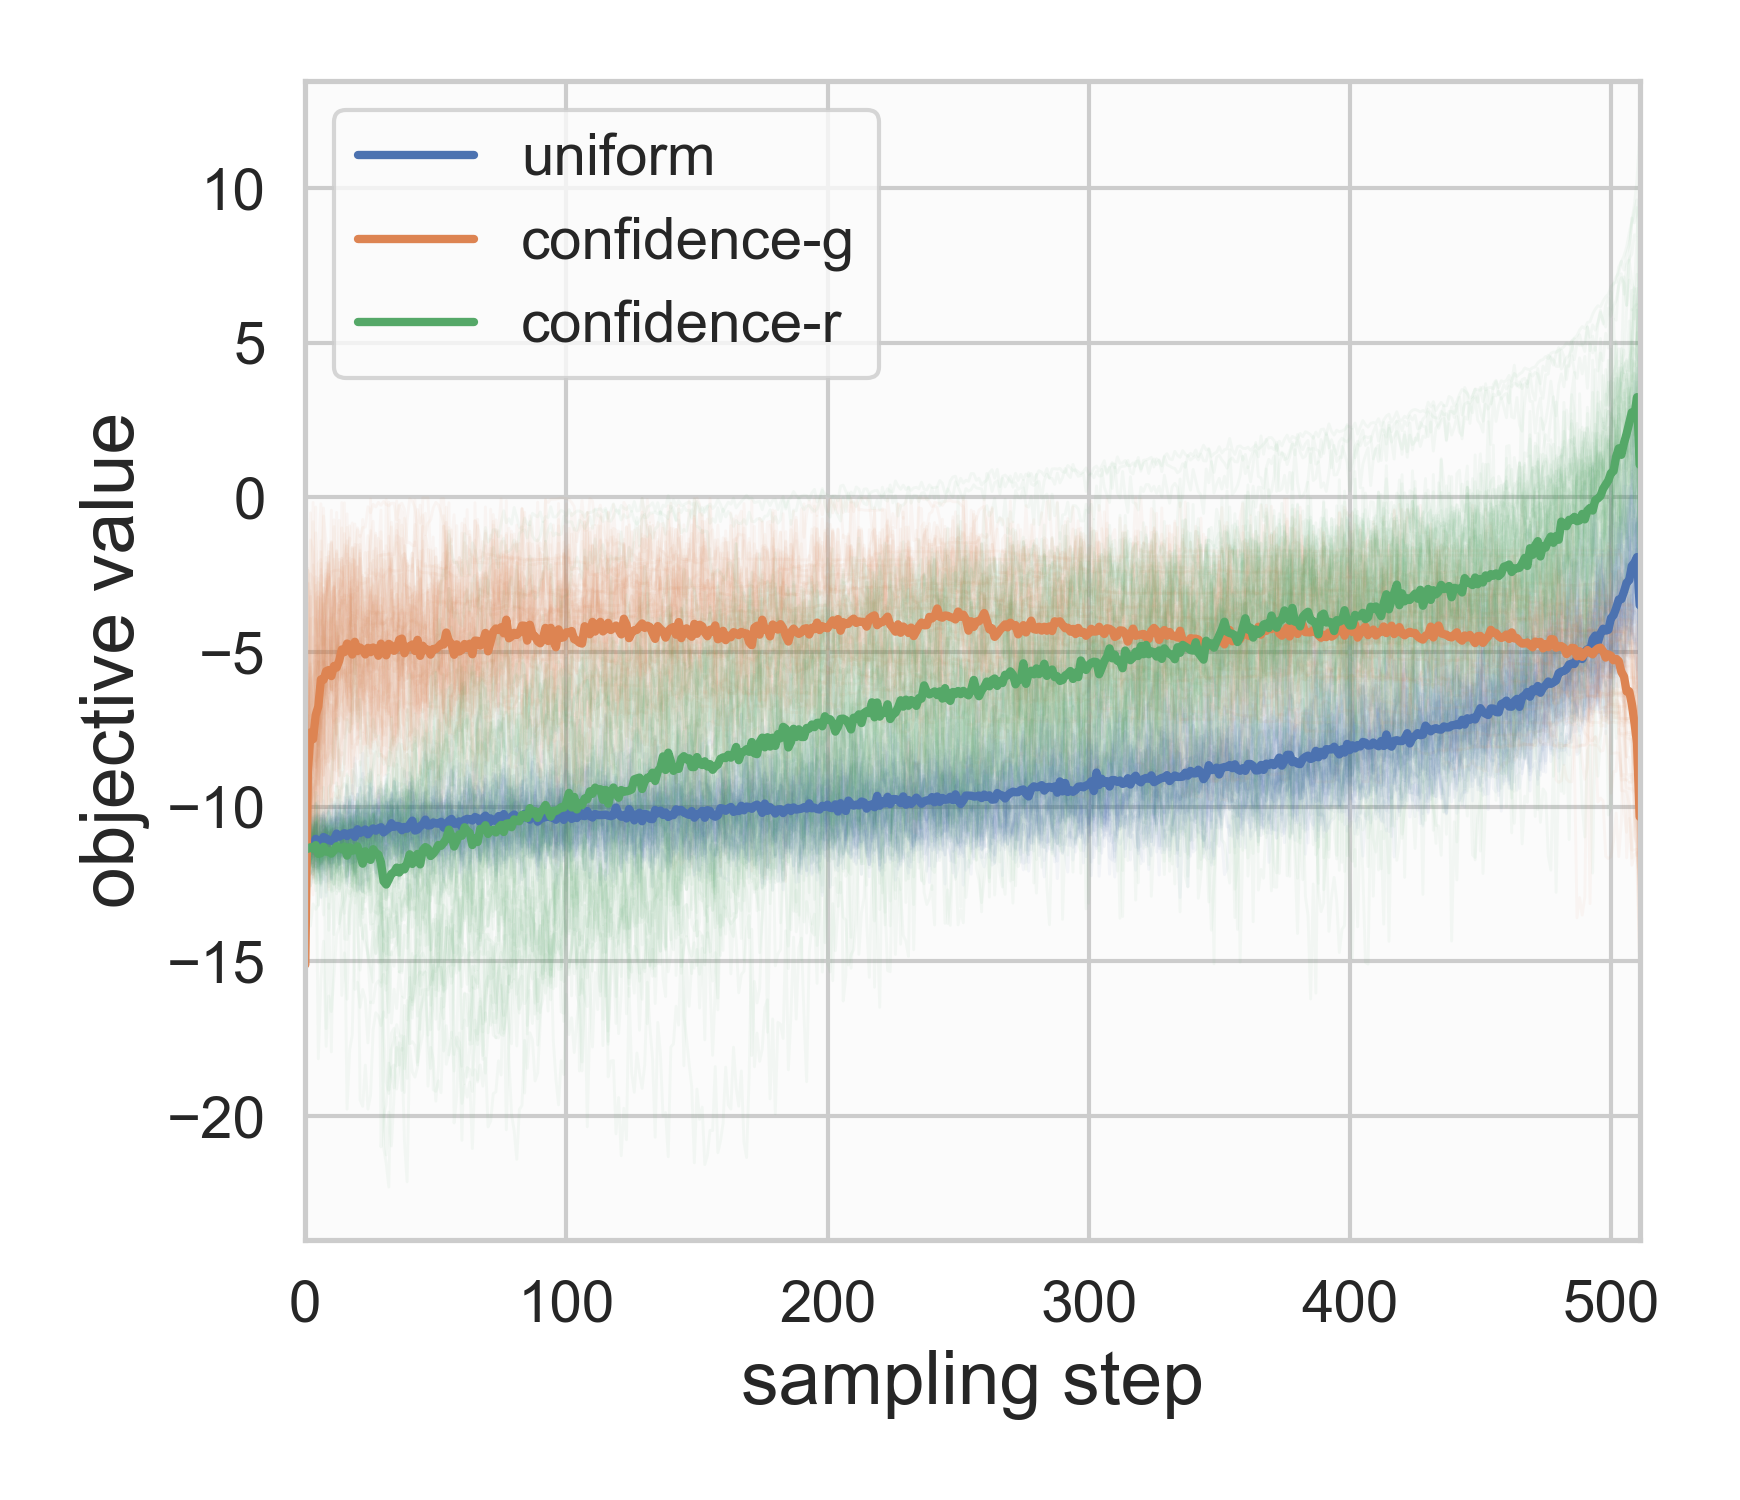
\includegraphics[width=\linewidth]{figs/objective_steps_512.png}
        \caption{Per-step objective values attained by unmasking strategies.}
        \label{fig:radd-obj-val}
    \end{subfigure}
    \label{fig:optimality-exp}
    \caption{Likelihood optimality analysis of unmasking strategies. \textbf{(a)}: The landscape of the local likelihood maximization problem \eqref{eq:trainable_confidence} over the policy simplex, under the synthetic task of unmasking 2 tokens from a length-3 sequence. We also plot different unmasking methods in the simplex and report their attained objective values. \textbf{(b)}: Monte Carlo estimation of local objective values \eqref{eq:trainable_confidence} attained by different unmasking methods in each step of 512-step text generation with RADD~\citep{ou2025absorbingdiscretediffusionsecretly}.}
\end{figure}

\paragraph{Landscape Visualization under Synthetic Distribution.}

We consider a task of unmasking 2 tokens from a length-3 sequence. There are exactly three possible unmasking actions: unmasking indices $\{0,1\}$, $\{0,2\}$, or $\{1,2\}$, enabling a full visualization of the optimization landscape in 3-dimensional space. To simulate MDM predictions $p_t^\theta(\cdot \mid \bm x_t)$, we use a synthetic distribution; see details in Appendix~\ref{subsec:synthetic}. In Figure~\ref{fig:opt-intro}, we plot the landscape and each unmasking method on the policy simplex. The exact optimizer of \eqref{eq:trainable_confidence} ($\bigstar$) is close to the entropy-based greedy point ($\blacktriangle$) with highly matching objective values, demonstrating Theorem~\ref{thm:confidence} and Theorem~\ref{thm:confidence-rand}. We provide additional results in Appendix~\ref{subsec:synthetic}. 

\paragraph{Objective Values in Real Text Generation.} 

We also evaluate the local objective value \eqref{eq:trainable_confidence} attained by different unmasking strategies in text generation using RADD~\citep{ou2024your}, a pretrained MDM. We compare uniform unmasking, greedy confidence unmasking based on the top-2 probability margin, and the randomized version. At each step, the objective \eqref{eq:trainable_confidence} is approximated by Monte Carlo estimation; see Appendix~\ref{subsec:radd-gen-exp}. In Figure~\ref{fig:radd-obj-val}, we set generation length to be 1024 and consider 512 diffusion sampling steps. We observe that both confidence methods consistently achieve higher objective values than the uniform method, in consistency with our theory in Section~\ref{sec:confidence}. See Appendix~\ref{subsec:radd-gen-exp} for further results.

\subsection{Evaluation of VLP}

\subsubsection{Text Generation}


\begin{wraptable}{r}{0.55\textwidth}
\caption{Average perplexity ($\downarrow$) of unconditional generations from RADD under different unmasking strategies and numbers of sampling steps. All generations have context length 1024.}
\centering
\small
\begin{tabular}{cccccc}
\toprule
steps & 16 & 32 & 64 & 128 & 256 \\
\midrule
uniform
& 335.1
& 199.7
& 154.5
& 132.2
& 118.9 \\
confidence-g
& 836.3
& 800.0
& 618.5
& 782.0
& 644.3 \\
confidence-r
& 308.7
& 186.3
& 132.4
& \textbf{109.2}
& \textbf{103.4} \\
\midrule
\cellcolor{lightblue}\alg{}
& \cellcolor{bestgreen}\textbf{293.2}
& \cellcolor{bestgreen}\textbf{179.6}
& \cellcolor{bestgreen}\textbf{130.3}
& \cellcolor{lightblue}116.9
& \cellcolor{lightblue}106.7 \\
\bottomrule
\end{tabular}
\label{tab:text-gen}
\end{wraptable}

For text generation, we evaluate \alg{} on RADD~\citep{ou2025absorbingdiscretediffusionsecretly}, a pretrained MDM for unconditional text generation. We train the unmasking policy on OpenWebText and evaluate generation quality using GPT-2 perplexity over sampling budgets from 16 to 256 steps. We compare against uniform unmasking and confidence unmasking based on top-2 probability margin, including both greedy and randomized variants. The detailed training and evaluation setup is provided in Appendix~\ref{sec:code-math-details}.

We report the GPT-2 perplexity of generated samples in Tables~\ref{tab:text-gen}. \alg{} substantially improves over uniform unmasking and matches or outperforms confidence-based methods, with the largest gains in the low-step regime. Randomized confidence unmasking is consistently stronger than greedy confidence unmasking, suggesting that deterministic high-confidence selection can be suboptimal.

\iffalse
\subsubsection{Code and Math Generation with DiffuCoder}
For code generation, we train our policy with DiffuCoder-7B-Instruct \citep{gong2025diffucoderunderstandingimprovingmasked}, a 7B-parameter MDM with strong coding performance after supervised fine-tuning on OpenCoder-SFT. The architecture of the policy network follows Section~\ref{subsec:architecture} and is approximately 1.5\% of the size of DiffuCoder. The policy is trained on the same SFT dataset. We reformat each query-output pair according to the chat template in Table~\ref{tab:chat-sft}, Appendix~\ref{sec:experiment-appendix}, following \citet{gong2025diffucoderunderstandingimprovingmasked}, and pad each chat to fixed length 1024 using DiffuCoder's padding token \texttt{<|dlm\_pad|>}. Following standard SFT practice for MDMs \citep{ye2025dream7bdiffusionlarge,nie2025largelanguagediffusionmodels,gong2025diffucoderunderstandingimprovingmasked}, we keep the prompt section intact during the masking and unmasking processes. We choose $K=16$ sampling steps, learning rate $\eta=0.001$, and $\lambda=0.1$ with AdamW optimizer.

We evaluate code generation using Pass@1 ($\uparrow$) on HumanEval \citep{chen2021evaluatinglargelanguagemodels} and MBPP \citep{austin2021programsynthesislargelanguage}. The evaluation chat templates are provided in Appendix~\ref{sec:experiment-appendix}. Results are reported in Table~\ref{tab:code-gen-diffucoder}. As in text generation, \alg{} consistently improves over uniform unmasking and outperforms confidence-based methods in most settings. Greedy confidence unmasking again performs poorly.

To examine whether the learned policy generalizes beyond coding, we additionally evaluate zero-shot math performance on GSM8K and MATH500 using the same DiffuCoder policy. Results are reported in Table~\ref{tab:math-diffucoder}. Since DiffuCoder is supervised-finetuned primarily on coding data, its absolute performance on math tasks is limited. Nevertheless, VLP remains competitive with or better than confidence-based unmasking at small and moderate step counts, indicating that the learned unmasking policy can transfer across domains.




\subsubsection{Broader Evaluation on Dream}
To better assess the behavior of the learned policy on models with stronger math ability, we additionally evaluate our method on Dream-7B \citep{ye2025dream7bdiffusionlarge}. Table~\ref{tab:dream-code} reports coding results on HumanEval and MBPP, while Table~\ref{tab:dream-math} reports math results on GSM8K and MATH500.

On coding benchmarks, the same trend holds: the learned policy improves over the model's original sampling strategy and generally outperforms confidence-based unmasking. On math benchmarks, VLP matches or surpasses confidence unmasking in most settings. These results strengthen the claim that VLP is not limited to DiffuCoder or coding-only tasks, but can transfer across models and domains.



\begin{table*}[h]
\centering
\caption{Results ($\uparrow$) of Dream-7B under different unmasking strategies and numbers of sampling steps across four benchmarks.}
\setlength{\tabcolsep}{4.5pt}
\resizebox{\textwidth}{!}{%
\begin{tabular}{ccccccccccccccccc}
\toprule
& \multicolumn{4}{c}{HumanEval} 
& \multicolumn{4}{c}{MBPP}
& \multicolumn{4}{c}{GSM8K}
& \multicolumn{4}{c}{MATH500} \\
\cmidrule(lr){2-5}\cmidrule(lr){6-9}\cmidrule(lr){10-13}\cmidrule(lr){14-17}
steps
& 16 & 32 & 64 & 128
& 16 & 32 & 64 & 128
& 16 & 32 & 64 & 128
& 16 & 32 & 64 & 128 \\
\midrule
uniform
& 8.5 & 17.6 & 19.5 & 23.2
& 18.6 & 25.6 & 27.6 & 30.8
& 23.4 & 30.0 & 34.9 & 35.4
& 10.4 & 12.8 & 13.8 & 16.8 \\
confidence-g
& 3.0 & 5.5 & 14.0 & 20.7
& 1.4 & 1.6 & 6.4 & 13.6
& 12.8 & 29.4 & \textbf{42.1} & \textbf{40.7}
& 3.6 & 7.0 & 15.0 & 12.0 \\
confidence-r
& 15.2 & 18.3 & 26.2 & 27.4
& \textbf{25.2} & 24.4 & 27.4 & 32.0
& 32.7 & 36.5 & 39.2 & 39.6
& 15.2 & 16.8 & 16.6 & 18.2 \\
\midrule
\cellcolor{lightblue}VLP
& \cellcolor{bestgreen}\textbf{17.0} & \cellcolor{bestgreen}\textbf{22.6} & \cellcolor{bestgreen}\textbf{27.4} & \cellcolor{bestgreen}\textbf{29.3}
& \cellcolor{lightblue}22.8 & \cellcolor{bestgreen}\textbf{26.2} & \cellcolor{bestgreen}\textbf{31.6} & \cellcolor{bestgreen}\textbf{32.8}
& \cellcolor{bestgreen}\textbf{33.6} & \cellcolor{bestgreen}\textbf{36.6} & \cellcolor{lightblue}38.3 & \cellcolor{lightblue}38.2
& \cellcolor{bestgreen}\textbf{15.6} & \cellcolor{bestgreen}\textbf{17.0} & \cellcolor{bestgreen}\textbf{17.2} & \cellcolor{bestgreen}\textbf{19.4} \\
\bottomrule
\end{tabular}%
}
\label{tab:dream-all}
\end{table*}

\fi


\subsubsection{Code and Math Generation}

We evaluate \alg{} on code and math generation using two 7B-scale MDMs: Dream-7B~\citep{ye2025dream7bdiffusionlarge} and DiffuCoder-7B~\citep{gong2025diffucoderunderstandingimprovingmasked}. We train the policy with OpenCoder-SFT and MetaMathQA dataset, and evaluate on two code generation benchmarks: HumanEval~\citep{chen2021evaluatinglargelanguagemodels} as well as MBPP~\citep{austin2021programsynthesislargelanguage}, and two math generation benchmarks: GSM8K~\citep{?} and MATH500~\citep{?}. The detailed setup is provided in Appendix~\ref{sec:vlp}.

Results on both models are summarized in Tables~\ref{tab:dream-all} and~\ref{tab:diffucoder-all} (deferred to Appendix~\ref{sec:vlp-additional-results}). Across Dream and DiffuCoder, \alg{} consistently matches or outperforms confidence-based unmasking, especially at small and moderate sampling budgets. Both \alg{} and random confidence method display a clear improvement from the vanilla uniform unmasking. Greedy confidence unmasking often performs poorly, suggesting that deterministic confidence selection can be suboptimal. These results indicate that likelihood-trained unmasking policies can provide robust gains across various models, sampling budgets, and task domains.

\begin{table*}[h]
\centering
\caption{Results ($\uparrow$) of Dream-7B under different unmasking strategies and numbers of sampling steps across four benchmarks.}
\setlength{\tabcolsep}{4.5pt}
\resizebox{\textwidth}{!}{%
\begin{tabular}{ccccccccccccccccc}
\toprule
& \multicolumn{4}{c}{HumanEval} 
& \multicolumn{4}{c}{MBPP}
& \multicolumn{4}{c}{GSM8K}
& \multicolumn{4}{c}{MATH500} \\
\cmidrule(lr){2-5}\cmidrule(lr){6-9}\cmidrule(lr){10-13}\cmidrule(lr){14-17}
steps
& 16 & 32 & 64 & 128
& 16 & 32 & 64 & 128
& 16 & 32 & 64 & 128
& 16 & 32 & 64 & 128 \\
\midrule
uniform
& 8.5 & 17.6 & 19.5 & 23.2
& 18.6 & 25.6 & 27.6 & 30.8
& 23.4 & 30.0 & 34.9 & 35.4
& 10.4 & 12.8 & 13.8 & 16.8 \\
confidence-g
& 3.0 & 5.5 & 14.0 & 20.7
& 1.4 & 1.6 & 6.4 & 13.6
& 12.8 & 29.4 & \textbf{42.1} & \textbf{40.7}
& 3.6 & 7.0 & 15.0 & 12.0 \\
confidence-r
& 15.2 & 18.3 & 26.2 & 27.4
& \textbf{25.2} & 24.4 & 27.4 & 32.0
& 32.7 & 36.5 & 39.2 & 39.6
& 15.2 & 16.8 & 16.6 & 18.2 \\
\midrule
\cellcolor{lightblue}VLP
& \cellcolor{bestgreen}\textbf{17.0} & \cellcolor{bestgreen}\textbf{22.6} & \cellcolor{bestgreen}\textbf{27.4} & \cellcolor{bestgreen}\textbf{29.3}
& \cellcolor{lightblue}22.8 & \cellcolor{bestgreen}\textbf{26.2} & \cellcolor{bestgreen}\textbf{31.6} & \cellcolor{bestgreen}\textbf{32.8}
& \cellcolor{bestgreen}\textbf{33.6} & \cellcolor{bestgreen}\textbf{36.6} & \cellcolor{lightblue}38.3 & \cellcolor{lightblue}38.2
& \cellcolor{bestgreen}\textbf{15.6} & \cellcolor{bestgreen}\textbf{17.0} & \cellcolor{bestgreen}\textbf{17.2} & \cellcolor{bestgreen}\textbf{19.4} \\
\bottomrule
\end{tabular}%
}
\label{tab:dream-all}
\end{table*}

\subsubsection{Ablation Studies}

\paragraph{Effect of KL regularization.}

\paragraph{Choice of $K$ in training.}


\section{Conclusion}
In this work, we study inference in masked diffusion language models through a likelihood-based formulation that treats the unmasking order as a policy to be optimized. Under local planning and distribution-approximation reductions, this framework explains confidence-based unmasking as an near-optimal policy, with numerical evidence supporting the likelihood-optimality view. Building on the same principle, we introduced Variational Likelihood Policy (\alg{}), a trainable unmasking policy optimized by a variational lower bound, and showed that it matches or improves over uniform and confidence-based unmasking across text, code, and math generation tasks and multiple MDMs at different scales.

This work still has several limitations. The theoretical derivation relies on local reductions and approximation assumptions, while the design of VLP is prototypical and can face inefficiency and instability in training. Future work may improve the optimization of VLP, explore joint training with the underlying diffusion model, and extend the likelihood principle to other discrete diffusion models beyond MDMs.

% \section*{Impact Statement}

% This paper presents work whose goal is to advance the field of machine learning. There are many potential societal consequences of our work, none of which we feel must be specifically highlighted here.

% For NeurIPS final versions, acknowledgments should use the ack environment.
% Do not include acknowledgments in the anonymized submission.
% \begin{ack}
% Acknowledgments go here.
% \end{ack}

\newpage

{\small
\bibliographystyle{plainnat}
\bibliography{main}
}

% \newpage
% \input{checklist.tex}

\newpage
\appendix
\appendix

\section{Additional Background and Preliminaries}\label{sec:literature-appendix}

\paragraph{Backward unmasking process of MDMs.}
It is known that the time reversal of a CTMC with rate $Q_t$ is also a CTMC, whose infinitesimal transition probability takes a form analogous to \eqref{eq:infinitesimal_transition}:
\begin{equation}
\label{eq:infinitesimal_transition_rev}
    q_{t-\Delta t|t}(\vy|\vx_t)  =  \delta(\vx_t, \vy) + \tilde{Q}_t(\vx_t, \vy) \Delta t + o(\Delta t).
\end{equation}
Here, $\tilde Q_t$ is an unknown transition rate. Specifically for MDMs, the reverse transition is an unmasking process \citep{lou2024discrete,campbell2022continuous,ou2025absorbingdiscretediffusionsecretly}, where we begin from an all-mask sequence and randomly unmask each to a token in the vocabulary with the following token level transitions:
\begin{align*}
    q_{s|t}\!\left(x_s^{i}|\bm x_t\right)
=
&\quad \begin{cases}
1,
& x_t^{i} \neq \mask,\; x_s^{i} = x_t^{i}, \\
\dfrac{1 - e^{-\bar{\sigma}(s)}}{1 - e^{-\bar{\sigma}(t)}},
& x_t^{i} = \mask,\; x_s^{i} = \mask, \\
\dfrac{e^{-\bar{\sigma}(s)} - e^{-\bar{\sigma}(t)}}{1 - e^{-\bar{\sigma}(t)}}\,
q_{0 | t}\!\left(x_s^{i}|x_t\right),
& x_t^{i} = \mask,\; x_s^{i} \neq \mask, \\
0,
& \text{otherwise}.
\end{cases}
\end{align*}
Therefore, the learning of the backward process reduces to the learning of the reverse rate $\tilde Q_t$ parameterized by a neural network with weight $\theta$. The training can be implemented by various approaches, such as by minimizing score-based objectives \citep{lou2024discrete,ou2025absorbingdiscretediffusionsecretly}. In this way, we have a parameterized approximation of the true backward rate $P_t^\theta\approx \tilde Q_t$, which leads to a marginal distribution $p_t^\theta$ at time $t$ by solving the Kolmogorov ODE $dp^\theta_t/dt=p_t^\theta P_t^\theta$.

\paragraph{Trainable inference methods for MDMs.}
Beyond fixed heuristics, several works treat the unmasking order as a trainable policy. Some introduce a separate policy network to learn update sequences \citep{peng2025path, jazbec2025learning, chen2025dultra} or introduce an additional MDM training stage on the preferred trajectories \citep{song2025seeddiffusionlargescalediffusion}, while others modify the backward process itself to encourage more structured updates, such as jointly updating semantically related variables \citep{meshchaninov2025guided} or incorporating corrective refinement steps for already unmasked tokens \citep{zhao2024informed}. These methods demonstrate that learning the inference procedure can significantly improve sample quality, but most existing approaches rely on rewards (reinforcement learning) or ad hoc update rules. Based on sample likelihood maximization, \citet{wang2025learningorder} proposes a framework to learn the optimal decoding order for any-order autoregressive models \citep{shih2022traininginferenceanyorderautoregressive}, which are limited to single-token generation processes; our \alg{} extends this framework to multi-token unmasking in masked diffusion models. From a related likelihood-based perspective, \citet{turok2026duel} restrict attention to deterministic position selection and obtain exact test-time likelihoods within this class. 

\section{Proofs}
\subsection{Preparation}
Consider an indexing of subsets $j\mapsto\mathcal U_j$ for all the size-$N$ subsets $\mathcal U_j$ of $[L]$. We denote $\bm\pi\in\mathbb R^{\binom{L}{N}}$ a probability vector such that $\pi_j:=\pi(\mathcal U_j|\bm x_k)$. Similarly, we denote $\bm z\in\mathbb R^{\binom{L}{N}}$ a random vector such that $z_j:=\prod_{i\in\mathcal U_j}p_{t_k}^{\theta,\pi}(x^i|\bm x_k)$, with the randomness $x^i\sim p_{t_k}^{\theta,\pi}(\cdot|\bm x_k)$. Then, \eqref{eq:trainable_confidence} becomes the following optimization problem over the probability simplex $\Delta$:
\begin{align}\label{eq:obj-equiv}
    \min_{\bm\pi\in\Delta}f(\bm\pi):=-\EE\log(\bm z^\top\bm\pi).
\end{align}

\subsection{Proof of Theorem \ref{thm:confidence}}\label{subsec:proof-confidence}
\begin{proof}
\textbf{Condition (1).} If $\pi$ is restricted to be a deterministic policy, then the optimal $\bm\pi^*=\bm e_j$ for some standard basis vector $\bm e_j$. Taking this to \eqref{eq:obj-equiv}, 
\begin{align*}
f(\bm\pi^*)&=-\EE\log z_j=-\EE_{\bm x\sim p_{t_k}^\theta(\cdot|\bm x_k)}\log\prod_{i\in\mathcal U_j}p_{t_k}^\theta(x^i|\bm x_k)\\
&=-\sum_{i\in\mathcal U_j}\sum_{v\in\mathcal V} p_{t_k}^\theta(x^i=v|\bm x_k)\log p_{t_k}^\theta(x^i=v|\bm x_k)=\sum_{i\in\mathcal U_j}H_k(i).
\end{align*}
Therefore, the minimum must be attained at the policy that deterministically outputs $\mathcal U^*$ with the smallest total entropy.

\textbf{Condition (2).} By \citet{cover1987log}, the KKT optimality conditions state that for an optimal $\bm\pi^*$,
\begin{align*}
    \EE\left[\frac{z_j}{\bm z^\top\bm\pi^*}\right]\begin{cases}
        =1,&\text{if }\bm\pi^*_j>0,\\
        \leq1,&\text{if }\bm\pi^*_j=0.
    \end{cases}
\end{align*}
Thus, if $\bm e_k$ is optimal for some $k$, then $\EE[z_j/z_k]\leq1$ for all $j$. Moreover, since there exists strictly feasible $\bm\pi$ in the probability simplex, Slater's condition holds and KKT optimality is necessary and sufficient. Thus an optimal $\bm\pi^*$ must be deterministic, and we have the same result as in Condition (1).

\end{proof}

\begin{remark}
A related entropy criterion appears independently in \citet{benhamu2025eb}: their EB-Sampler unmasks token subsets satisfying an entropy-difference bound $\sum_{l\in\mathcal U}H_k(l)-\max_{l\in\mathcal U}H_k(l)\leq\gamma$, motivated as an upper bound on joint dependence error in a KL-based analysis of MDM sampling. Theorem~\ref{thm:confidence} provides a complementary justification: under our locality restriction, entropy-greedy unmasking is the optimal stochastic policy for likelihood maximization, giving a likelihood-theoretic foundation for the use of entropy as the unmasking signal.
\end{remark}

\begin{remark}
The optimization framework underlying Theorem~\ref{thm:confidence} naturally extends to other confidence-based heuristic samplers by augmenting \eqref{eq:trainable_confidence} with additional data-dependent constraints on the policy. Provided such constraints act separably on the feasible simplex of $\pi(\cdot|\bm x_k)$ and preserve convexity, the KKT analysis carries through on the restricted region, and the optimal policy reduces to entropy-greedy unmasking within the constrained subset. We illustrate this with KLASS \citep{kim2025klass} in Appendix~\ref{subsec:klass-extension}.
\end{remark}

\subsection{Worked Example: KLASS as a Constrained Instance}\label{subsec:klass-extension}

We illustrate how the framework underlying Theorem~\ref{thm:confidence} extends to other confidence-based heuristic samplers, using KLASS \citep{kim2025klass} as a representative example. KLASS augments confidence unmasking with a KL-stability filter: at each step $k$, it scores each masked position by the KL divergence between the predicted vocabulary distribution at $\bm x_k$ and predictions from a recent history window, and restricts unmasking to the stable subset
\begin{align*}
    S_k = \{i \in [L] : x_k^i = \mask,\ \text{position } i \text{ is KL-stable over the history window}\} \subseteq [L].
\end{align*}
Within this stable set, KLASS unmasks the highest-confidence positions.

In our framework, this restriction amounts to constraining the support of $\pi(\cdot | \bm x_k)$ to subsets $\mathcal U \subseteq S_k$. Following the indexing of Appendix~\ref{subsec:proof-confidence}, let $J(S_k) := \{j : \mathcal U_j \subseteq S_k\}$, and let
\begin{align*}
    \Delta_{S_k} := \{\bm\pi \in \Delta : \pi_j = 0 \text{ for all } j \notin J(S_k)\}
\end{align*}
denote the induced sub-simplex. The KLASS-constrained version of \eqref{eq:trainable_confidence} is then
\begin{align}\label{eq:klass-obj}
    \min_{\bm\pi \in \Delta_{S_k}} f(\bm\pi) = -\EE\log(\bm z^\top \bm\pi),
\end{align}
which differs from \eqref{eq:obj-equiv} only in its feasible set.

\begin{proposition}\label{prop:klass}
Under the conditions of Theorem~\ref{thm:confidence}, with $|S_k| \geq N$, the optimal solution to \eqref{eq:klass-obj} is $\bm\pi^* = \bm e_{j^*}$ where
\begin{align*}
    \mathcal U^* = \argmax_{\mathcal U \subseteq S_k,\, |\mathcal U| = N} \sum_{i \in \mathcal U} -H_k(i),
\end{align*}
recovering the unmasking rule of KLASS.
\end{proposition}

\begin{proof}
$\Delta_{S_k}$ is itself a probability simplex, supported on $J(S_k)$. The KKT analysis in the proof of Theorem~\ref{thm:confidence} applies verbatim with the index $j$ ranging over $J(S_k)$ rather than the full set, since the stationarity condition is separable across coordinates and the constraint $\bm\pi \in \Delta_{S_k}$ preserves convexity. The optimum is therefore attained at a vertex $\bm e_{j^*}$, with $j^*$ corresponding to the size-$N$ subset $\mathcal U^* \subseteq S_k$ that minimizes the total entropy $\sum_{i \in \mathcal U} H_k(i)$.
\end{proof}

The same reduction applies to any confidence-based sampler that imposes a data-dependent feasibility set $\mathcal U \in \mathcal C(\bm x_k)$ determined by the model's predictions (and not by $\pi$ itself). In each case, the optimal policy under the constrained objective is the entropy-greedy choice within $\mathcal C(\bm x_k)$.

\subsection{Proof of Theorem~\ref{thm:confidence-rand}}\label{subsec:proof-random}
\begin{proof}
The Hessian of the objective is
\begin{align*}
    \nabla^2f(\bm\pi)=\EE\left[\frac{\bm z\bm z^\top}{(\bm z^\top\bm\pi)^2}\right]\succeq\EE[\bm z\bm z^\top]=\bm\Sigma,
\end{align*}
for $(\bm z^\top\bm\pi)^2\leq\|\bm z\|_\infty^2\leq1$. Therefore, $\nabla^2f(\bm\pi)$ is positive-definite with smallest eigenvalue greater than $\lambda=\lambda_{\min}(\bm\Sigma)$. This means $f$ is $\lambda$-strongly convex, i.e. for any $\bm\pi,\bm\pi'$,
\begin{align*}
    f(\bm\pi)-f(\bm\pi')\geq\ip{\nabla f(\bm\pi'),\bm\pi-\bm\pi'}+\frac{\lambda}{2}\nm{\bm\pi-\bm\pi'}^2_2.
\end{align*}
Denoting $\hat{\bm\pi}=\bm e_{j^*}$ for $j^*$ corresponding to $\mathcal U^*$. By the above inequality we have
\begin{align}
    f(\hat{\bm\pi})-f(\bm \pi^*)&\leq\ip{\nabla f(\hat{\bm\pi}),\hat{\bm\pi}-\bm\pi^*}-\frac{\lambda}{2}\nm{\hat{\bm\pi}-\bm\pi^*}^2_2\nonumber\\
    &=\ip{\bm P\nabla f(\hat{\bm\pi}),\hat{\bm\pi}-\bm\pi^*}+\ip{\nabla f(\hat{\bm\pi})-\bm P\nabla f(\hat{\bm\pi}),\hat{\bm\pi}-\bm\pi^*}-\frac{\lambda}{2}\nm{\hat{\bm\pi}-\bm\pi^*}^2_2\nonumber\\
    &=\ip{\bm P\nabla f(\hat{\bm\pi}),\hat{\bm\pi}-\bm\pi^*}-\frac{\lambda}{2}\nm{\hat{\bm\pi}-\bm\pi^*}^2_2\label{eq:proj-eq-1}\\
    &\leq \nm{\bm P\nabla f(\hat{\bm\pi})}_2\nm{\hat{\bm\pi}-\bm\pi^*}_2-\frac{\lambda}{2}\nm{\hat{\bm\pi}-\bm\pi^*}_2^2\leq\frac{\nm{\bm P\nabla f(\hat{\bm\pi})}_2^2}{2\lambda}\label{eq:cauchy-ineq},
\end{align}
where \eqref{eq:proj-eq-1} is due to the fact that $\hat{\bm\pi}-\bm\pi^*$ lies in the projection hyperplane of $\bm P$, and \eqref{eq:cauchy-ineq} is due to Cauchy-Schwartz inequality and quadratic maximization. On the other hand, we also have
\begin{align*}
    f(\hat{\bm\pi})-f(\bm\pi^*)\geq\ip{\nabla f(\bm\pi^*),\hat{\bm\pi}-\bm\pi^*}+\frac{\lambda}{2}\nm{\hat{\bm\pi}-\bm\pi^*}^2_2=\frac{\lambda}{2}\nm{\hat{\bm\pi}-\bm\pi^*}^2_2,
\end{align*}
since $\bm\pi^*$ lies in the interior of $\Delta$ and the projected gradient should vanish at optimality \citep{wright2022optimization}. Combining this with \eqref{eq:cauchy-ineq} we have
\begin{align*}
    \nm{\hat{\bm\pi}-\bm\pi^*}_2\leq\frac{\nm{\bm P\nabla f(\hat{\bm\pi})}_2}{\lambda}.
\end{align*}
Since ${\hat{\bm\pi}}=\bm e_{j^*}$,
\begin{align*}
    1-\pi^*_{j^*}=\hat{\pi}_{j^*}-\pi^*_{j^*}\leq\nm{\hat{\bm\pi}-\bm\pi^*}_\infty\leq\nm{\hat{\bm\pi}-\bm\pi^*}_2,
\end{align*}
which completes the proof.
\end{proof}

\subsection{Proof of Theorem \ref{thm:confidence_bounds}}
\begin{proof}
    Let $F$ be the objective function
\begin{align*}
    F = -\EE_{\bm x_0\sim q(\cdot |\bm x_k)}\log \sum_{\mathcal U_k}\pi(\mathcal U_k|\bm x_k)\prod_{i\in\mathcal U_{k}}p^\theta_k(\bm x^i_{k-1}|\bm x_k),
\end{align*}
and let $G$ be the objective function
\begin{align*}
    G = -\EE_{\bm x_0\sim p^\theta_k(\cdot |\bm x_k)}\log \sum_{\mathcal U_k}\pi(\mathcal U_k|\bm x_k)\prod_{i\in\mathcal U_{k}}p^\theta_k(\bm x^i_{k-1}|\bm x_k).
\end{align*}
Note that we let the objective functions be the expected negative log-likelihood to enforce positivity on the objective values. From the bounds on the Renyi divergence, we have that for any $\pi$, we have
\begin{align*}
    |(F-G)(\pi)| &= \sum_{\bm x_0 \in \mathcal{V}^L}\log \sum_{\mathcal U_k}\pi(\mathcal U_k|\bm x_k)\prod_{i\in\mathcal U_{k}}p^\theta_k(\bm x^i_{k-1}|\bm x_k)(|p^\theta_k(\bm x_0|\bm x_k)-q(\bm x_0|\bm x_k)|)\\
    &\leq(e^\epsilon-1)\sum_{\bm x_0 \in \mathcal{V}^L}\log \sum_{\mathcal U_k}\pi(\mathcal U_k|\bm x_k)\prod_{i\in\mathcal U_{k}}p^\theta_k(\bm x^i_{k-1}|\bm x_k)p^\theta_k(\bm x_0|\bm x_k) \\
    &= (e^\epsilon-1)F(\pi),
\end{align*}
where the inequality comes from the fact that for any realization of $x_0$, we have the Renyi divergence implies,
\begin{align*}
    |p^\theta_k(\bm x_0|\bm x_k)-q_0(\bm x_0|\bm x_k)| &\leq (\max\{e^\epsilon-1, 1-e^{-\epsilon}\})q_0(\bm x_0|\bm x_k) \\
    &\leq (e^\epsilon-1)q_0(\bm x_0|\bm x_k).
\end{align*}
Now, note that $e^\epsilon-1 \leq 2\epsilon$ for $\epsilon \leq 1$, so for any $\pi$, we have
\begin{align*}
    (1-2\epsilon)F(\pi) \leq G(\pi) \leq (1+2\epsilon)F(\pi).
\end{align*}
By the symmetry of the Renyi bounds, we also have that
\begin{align*}
    (1-2\epsilon)G(\pi) \leq F(\pi) \leq (1+2\epsilon)G(\pi).
\end{align*}
Letting $\argmin_\pi F = \pi^\star$ and $\argmin_\pi G = \hat{\pi}$, we have
\begin{align*}
    F(\pi^\star)
\leq F(\hat{\pi})
\leq (1+2\epsilon)\,G(\hat{\pi})
\leq (1+2\epsilon)\,G(\pi^\star)
\leq (1+2\epsilon)^2\,F(\pi^\star),
\end{align*}
or in other words, 
\begin{align*}
    \frac{F(\hat{\pi})}{F(\pi^\star)} &\leq (1+2\epsilon)^2 \\
    &\leq 1+8\epsilon \quad \forall \epsilon \leq 1.
\end{align*}
Therefore, the gap between the two optimal policies in loss is bounded by the distance between $p^\theta_k$ and $q_0$. In other words, as long as the training distribution closely matches the original data distribution, the optimal policy under the former will not be far from the optimal policy under the latter.
\end{proof}
\iffalse
\subsection{Proof of Proposition \ref{prop:naive_elbo}}
\begin{proof}
    We can try to develop ELBO for $-\EE_{q_0}\log p_0^{\theta,\pi}(\bm x_0)$ for optimizing $\pi$. A negative discrete-time ELBO is given by 
\begin{align*}
    \EE_{q_0}\left[-\log p^{\theta, \pi}_{0}(\bm x_0)\right]&\geq \EE_{q_{0:K}}\left[-\log\frac{p_{0:K}^{\theta,\pi}(\bm x_{0:K})}{q_{1:K|0}(\bm x_{1:K}|\bm x_0)}\right]\\
    &:=\mathcal L_\text{DT}(\theta,\pi)
\end{align*}
and it is known that $\mathcal L_\text{DT}$ can be recast into aligning the backward process with the forward one in terms of KL divergence:
\begin{align*}
    \mathcal L_\text{DT}(\theta,\pi)&=\EE_{q_0}\left[\mathrm{KL}(q_{K|0}(\bm x_K|\bm x_0)||p_K^{\theta,\pi}(\bm x_K))-\EE_{q_{1|0}}\left[\log p_{0|1}^{\theta,\pi}(\bm x_0|\bm x_1)\right]\right]+\sum_{k=1}^{K-1}\mathcal L_k(\theta,\pi)
\end{align*}
with
\begin{align*}
    \mathcal L_k(\theta,\pi)
    &=\EE_{q_0q_{k+1|0}}\left[\mathrm{KL}\left(q_{k|k+1,0}(\bm x_k|\bm x_{k+1},\bm x_0)\middle\|p^{\theta, \pi}_{k+1}(\bm x_k|\bm x_{k+1})\right)\right]\\
    &=-\EE_{q_0q_{k+1|0}q_{k|k+1,0}}\left[\log p_{k+1}^{\theta,\pi}(\bm x_k|\bm x_{k+1})\right]+C\\
    &=-\EE_{q_0q_{k|0}q_{k+1|k}}\left[\log p_{k+1}^{\theta,\pi}(\bm x_k|\bm x_{k+1})\right]+C\\
    &=-\EE_{q_0q_{k|0}q_{k+1|k}}\left[\sum_{i\in\mathcal U}\log p^\theta_{t_k|t_{k+1}}(\bm x^i_k|\bm x_{k+1})+\log\pi(\mathcal U\,|\,t_{k+1},\Delta t,\bm x_{k+1})\right]
\end{align*}
Now, due to linearity of expectation, any optimal $\pi$ should give identical probability to any equal-sized $\mathcal U$ (because it should align with the forward process). This means we have no training signal at all for optimizing $\pi$. The mathematical intuition is that taking logarithm of a multiplicative term disentangles the interacting factors ($\pi$ and $p^\theta$).
\end{proof}
\fi
% First, note that
% \begin{align*}
% F(\hat{\pi}) &= G(\hat{\pi})  + (F-G)(\hat{\pi}) \\
% &\leq G(\pi^\star) + (F-G)(\hat{\pi}) \\
% &= F(\pi^\star) + (G-F)(\pi^\star) + (F-G)(\hat{\pi}) \\
% \implies 0 \leq F(\hat{\pi}) - F(\pi^\star) &\leq  (G-F)(\pi^\star) + (F-G)(\hat{\pi}).
% \end{align*}


% \subsection{Proof of Proposition \ref{prop:training}}
% \begin{proof}
% Fix $x_0$. For any distribution $r(\cdot\mid x_0)$ over $T$ with
% $r(T\mid x_0)>0$ whenever $A_\pi(T)>0$, we rewrite the trajectory sum as
% \begin{equation}
% \begin{split}
% \sum_T A_\pi(T)
% &= \sum_T r(T\mid x_0)\,\frac{A_\pi(T)}{r(T\mid x_0)} \\
% &= \mathbb E_{T \sim r(\cdot\mid x_0)}
% \left[\frac{A_\pi(T)}{r(T\mid x_0)}\right].
% \end{split}
% \end{equation}
% Since $\log$ is concave, Jensen's inequality implies
% \begin{equation}
% \begin{split}
% \log \sum_T A_\pi(T)
% &= \log \mathbb E_{T \sim r(\cdot\mid x_0)}
% \left[\frac{A_\pi(T)}{r(T\mid x_0)}\right] \\
% &\ge
% \mathbb E_{T \sim r(\cdot\mid x_0)}
% \left[
% \log A_\pi(T) - \log r(T\mid x_0)
% \right].
% \end{split}
% \end{equation}
% Taking expectation over $x_0 \sim q_0$ yields
% \begin{equation}
% \begin{split}
% \mathbb E_{x_0 \sim q_0}
% \log \sum_T A_\pi(T)
% \;\ge\;
% \mathbb E_{x_0 \sim q_0}\,
% \mathbb E_{T \sim r(\cdot\mid x_0)}
% \Big[
% \log A_\pi(T) - \log r(T\mid x_0)
% \Big].
% \end{split}
% \end{equation}
% Finally, observe that
% \begin{equation}
% \begin{split}
% \mathbb E_{T \sim r(\cdot\mid x_0)}
% [-\log r(T\mid x_0)]
% &= H\big(r(\cdot\mid x_0)\big)
% \;\ge\; 0.
% \end{split}
% \end{equation}
% Therefore, the looser bound
% \begin{equation}
% \begin{split}
% \mathbb E_{x_0 \sim q_0}
% \log \sum_T A_\pi(T)
% \;\ge\;
% \mathbb E_{x_0 \sim q_0}\,
% \mathbb E_{T \sim r(\cdot\mid x_0)}
% [\log A_\pi(T)]
% \end{split}
% \end{equation}
% also holds. Moreover, since the entropy term does not depend on $\pi$
% (when $r$ is fixed independently of $\pi$),
% maximizing this form of ELBO over $\pi$ is equivalent to maximizing
% $\mathbb E_{x_0}\mathbb E_{T\sim r}[\log A_\pi(T)]$.
% \end{proof}


\section{Further Details on VLP}\label{sec:further-vlp}
\subsection{Model Architecture}\label{subsec:architecture}
\begin{wrapfigure}{r}{0.42\textwidth}
    \vspace{-1.0em}
    \centering
    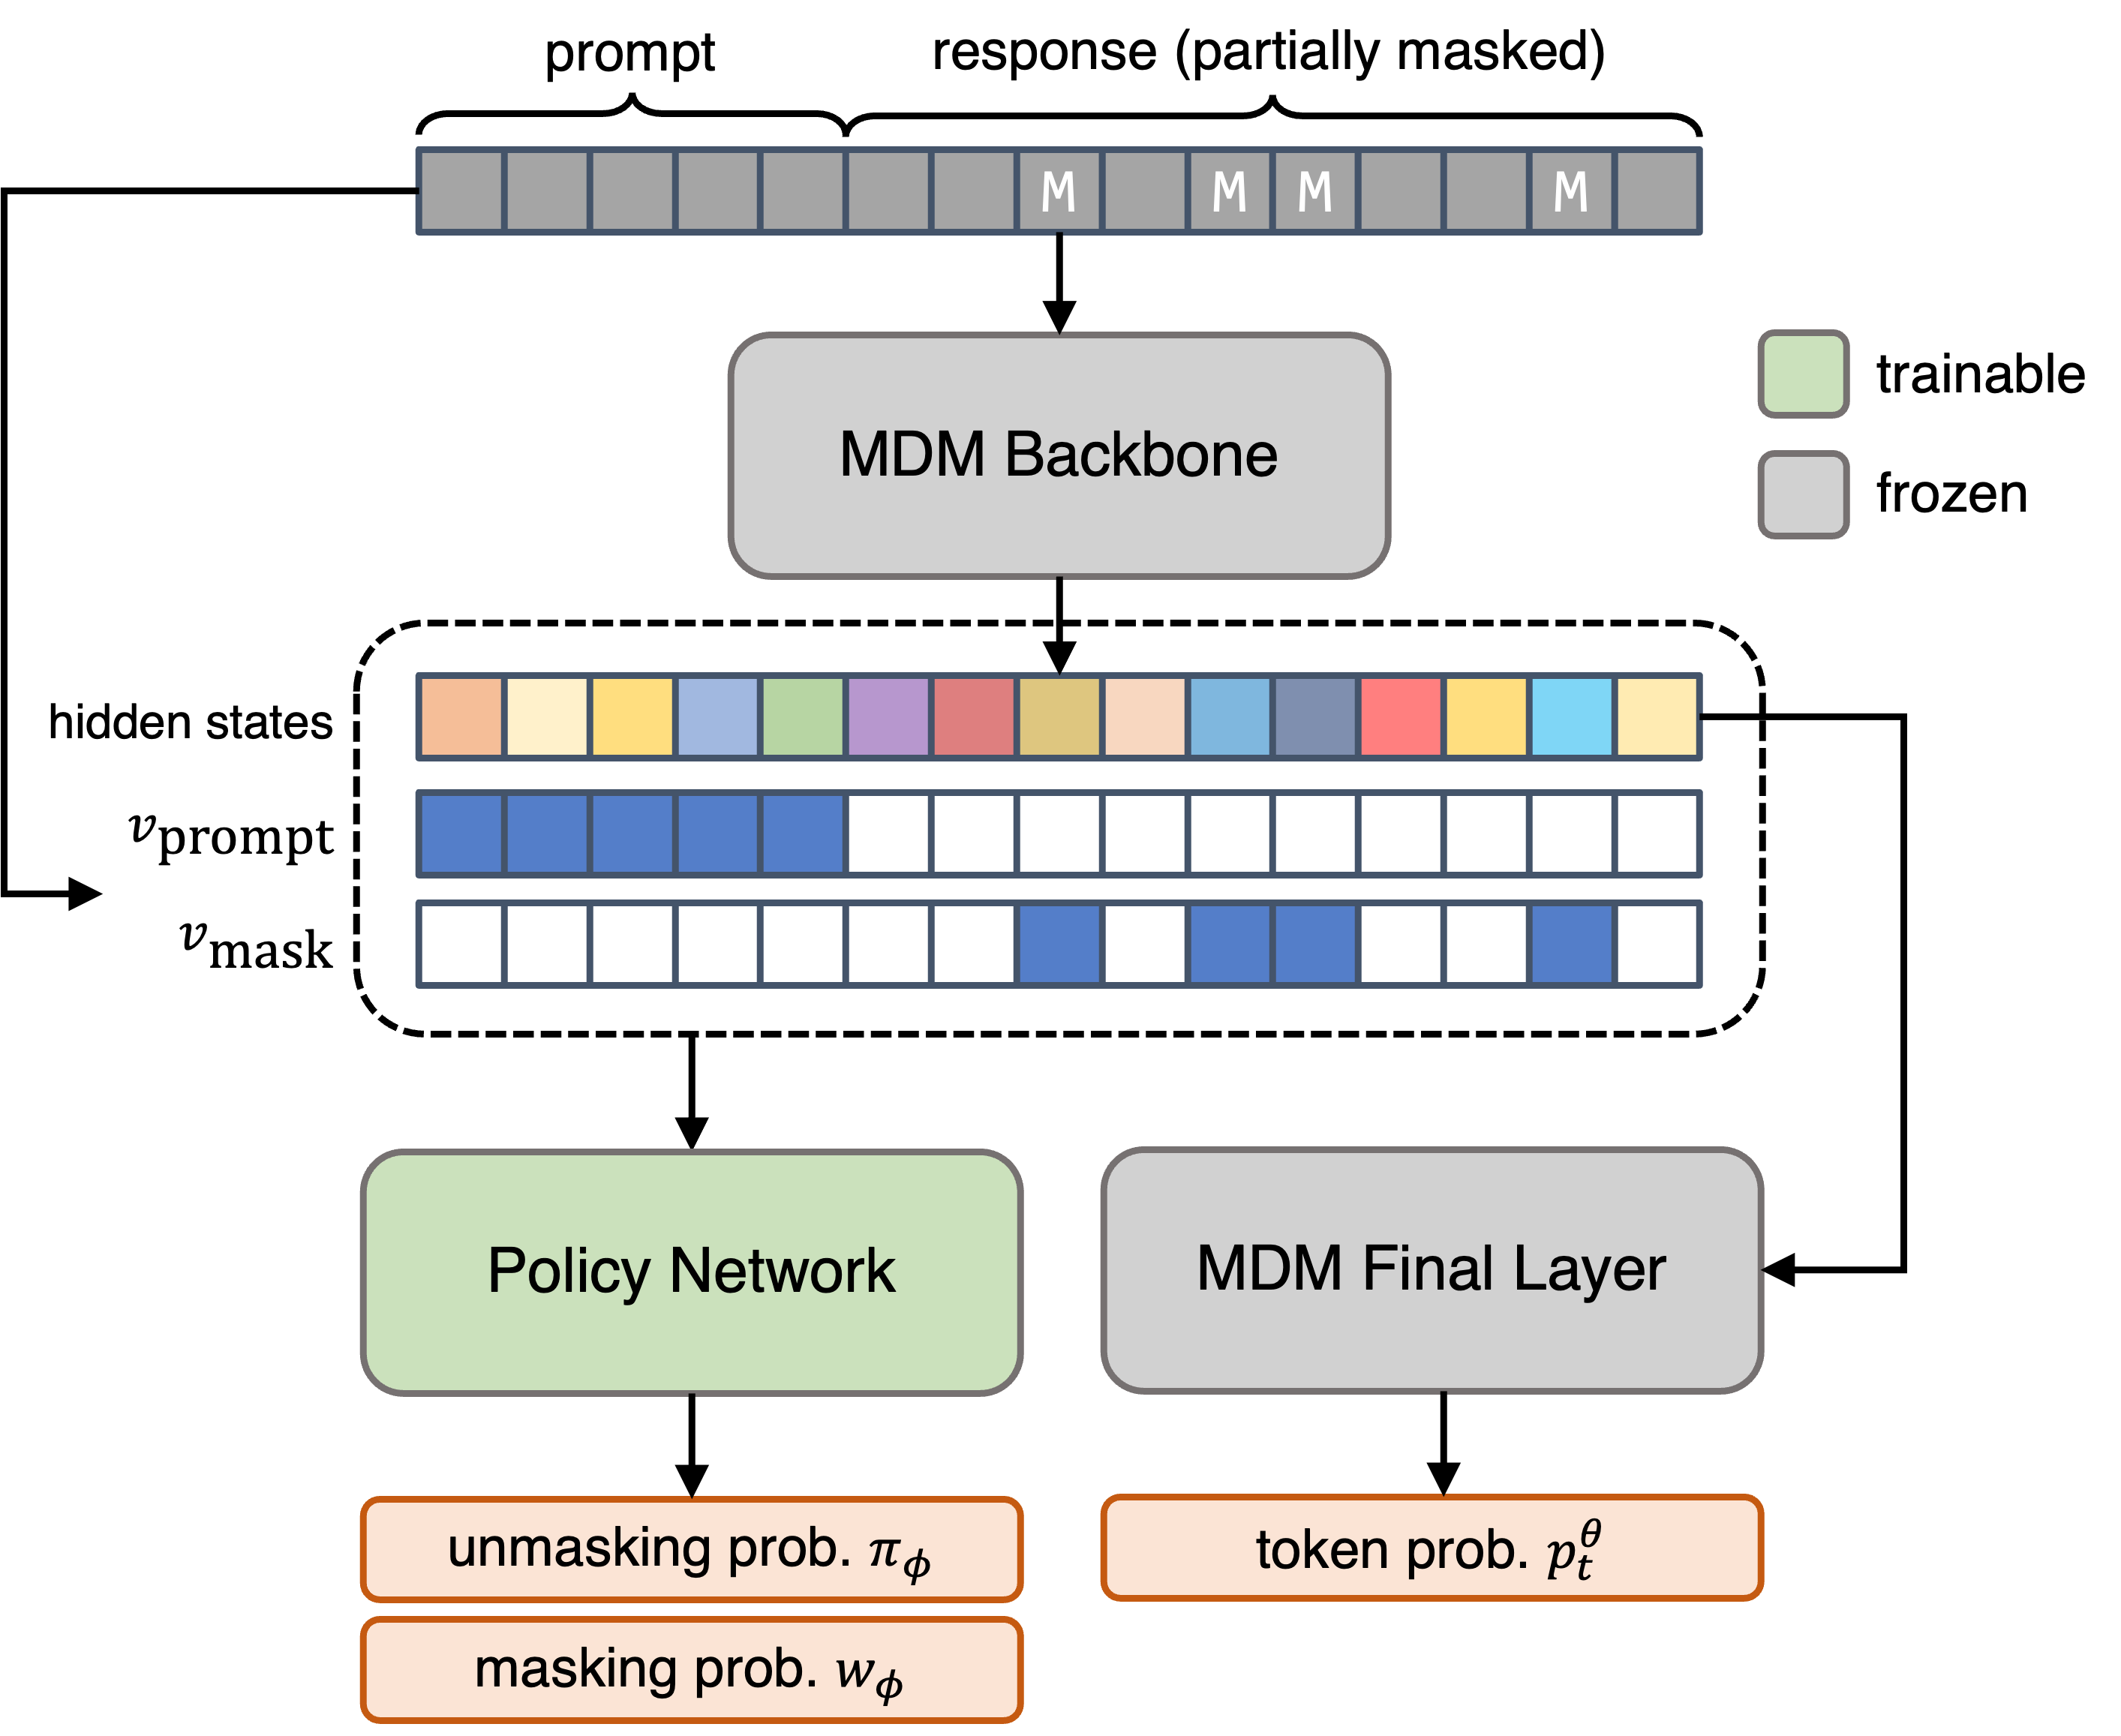
\includegraphics[width=\linewidth]{figs/vlp.png}
    \caption{An illustration of the shared-torso architecture of \alg{} with a trained MDM.}
    \label{fig:vlp}
    \vspace{-1.0em}
\end{wrapfigure}
To represent a policy $\pi_\phi$, we use a neural network that takes current sampling state $\bm x_{k}$ as input, and outputs a probability distribution over the size-$(L/K)$ index sets $\mathcal U_k$ for the next unmasking step. In our implementation, we adopt a shared-torso architecture: the policy network reuses the trained backbone of the MDM and appends an additional lightweight module. This reduces the number of trainable parameters: we pass the MDM's final-layer hidden states $\bm h_k$ to the policy in place of the raw tokens $\bm x_k$. A similar parameterization applies to the distribution $w$.

In our implementation, the additional module is a single-layer Transformer \citep{vaswani2017attention} block with bidirectional multi-head attention and rotary positional embedding \citep{su2023roformerenhancedtransformerrotary}. In addition to the hidden states $\bm h_{k}$, via concatenation, we also input two binary embeddings $\bm v_\text{mask}=(\mathbf1_{x_k^1=\mask},...,\mathbf1_{x_k^L=\mask})\in\{0,1\}^L$ and $\bm v_\text{prompt}=(\mathbf1_{x_k^1\text{ is prompt}},...,\mathbf1_{x_k^L\text{ is prompt}})\in\{0,1\}^L$ to explicitly provide the mask and prompt positions of the sequence. The output is a probability vector $\bm p=(p_1,...,p_L)$ through an application of the softmax function. It models a multinomial distribution over index sets, where each index $i$ is randomly selected to join $\mathcal U_k$ with probability $p_i$. We adopt the multinomial parameterization rather than independent per-position Bernoulli draws (as in, e.g., \citet{chen2025dultra}) since it natively models distributions over fixed-size index sets; in early experiments, an independent-Bernoulli variant collapsed toward unmasking very few tokens per step, since such low-cardinality outcomes have higher joint probability under the model. We illustrate the above design in Figure~\ref{fig:vlp}.

\iffalse
\subsection{Policy Parameterization with Gumbel Trick}
Recall that we constrain our policy to (randomly) output unmasking set of fixed size $N$. To this end, we make use of Gumbel Top-$N$ trick for efficient sampling and computation. Specifically, given policy network's output $\bm p=(p_1,p_2,...,p_L)\in\Delta([L])$, we randomly decide an index set $\mathcal U$ with $|\mathcal U|=N$ by sampling $\bm g\sim\mathrm{Gumbel(0,1)}$ and then pick the top-$N$ indices
\begin{align*}
    \mathcal U=\mathrm{top}_N(\log\bm p +\bm g).
\end{align*}
By this Gumbel sampling trick, the policy indeed assigns $\mathcal U$ with probability
\begin{align*}
    \pi(\mathcal U)&=\Pr\left(\min_{i\in\mathcal U}\log p_i+g_i>\max_{j\neq\mathcal U}\log  p_j+g_j\right)\\
    &=\int_0^\infty \prod_{i\in\mathcal U} p_ie^{-p_it}\prod_{j\notin\mathcal U}(1-e^{-p_jt})dt\\
    &=\int_0^1 \prod_{i\in\mathcal U} p_is^{p_i}\prod_{j\notin\mathcal U}(1-s^{p_j})\frac{1}{s}ds.
\end{align*}
Therefore we can compute an unbiased estimate for $\pi(\mathcal U)$.
\fi


\subsection{Training and Inference}
We summarize training and inference of \alg{} in Algorithm~\ref{alg:train} and~\ref{alg:inf}, respectively. In general, at each training iteration we draw a data sample $\bm x_0\sim q_0$, sample a masking trajectory from $w_\phi$, and compute the corresponding unmasking loss using $\pi_\phi$. Since $\phi$ also appears in the sampling of the masking trajectory from $w_\phi$, the stochastic gradients $\nabla_\phi s^{(i)}$ must be corrected via REINFORCE \citep{wang2025learningorder} to obtain an unbiased estimate $g_\text{REINFORCE}=\nabla_\phi s^{(i)}+(s^{(i)}-s)\nabla_\phi\log w^{(i)}$. While REINFORCE is known to have high gradient variance \citep{shi2022gradient}, we retain this estimator to maintain methodological compatibility with \citet{wang2025learningorder}, whose framework our work extends to multi-token unmasking. Lower-variance alternatives are left to future work. At the inference stage, we directly use the trained policy to sample an unmasking index set and apply the trained MDM to predict tokens.


\begin{algorithm}[tb]
  \caption{\alg{} Training}
  \label{alg:train}
  \begin{algorithmic}[1]
    \Input Initialization $\phi$, trained MDM $p^\theta_t$, dataset $\mathcal D$, batch size $B$, total sampling steps $K$, learning rate $\eta$, regularization strength $\lambda$
    \Output Trained policy $\pi_\phi$
    \Repeat
      \State Sample data batch $\{\bm x_0^{(i)}\}_{i=1}^B \sim \mathcal D$
      \For{$i=1,\ldots,B$}
        \State Sample $\mathcal U^{(i)} \sim w_\phi(\cdot \mid \bm x_0^{(i)})$
        \State Construct $\bm x_1^{(i)},\ldots,\bm x_K^{(i)}$ according to $\mathcal U^{(i)}$
        \State $w^{(i)} \gets w_\phi(\mathcal U^{(i)} \mid \bm x_0^{(i)})$
        \State $p^{(i)} \gets \prod_{k=1}^K
        p^\theta_{t_k}(\bm x_{k-1}^{(i)} \mid \bm x_k^{(i)})
        \pi_\phi(\mathcal U_{k}^{(i)} \mid \bm x_k^{(i)})$
        \State $r^{(i)} \gets
        \sum_{k=1}^K
        \mathrm{KL}\!\left(
        \pi_\phi(\cdot \mid \bm x_k^{(i)})
        \,\|\, 
        \pi_{\mathrm{ref}}(\cdot \mid \bm x_k^{(i)})
        \right)+
        \mathrm{KL}\!\left(
        w_\phi(\cdot \mid \bm x_0^{(i)})
        \,\|\,
        w_{\mathrm{ref}}(\cdot \mid \bm x_0^{(i)})
        \right)$
        \State $s^{(i)} \gets \log w^{(i)} - \log p^{(i)} + \lambda r^{(i)}$
      \EndFor
      \State $s \gets \frac{1}{B}\sum_{i=1}^B s^{(i)}$
      \State $g_{\text{REINFORCE}} \gets
      \frac{1}{B}\sum_{i=1}^B
      \left[
      \nabla_\phi s^{(i)}
      +
      \left(s^{(i)} - s\right)
      \nabla_\phi \log w^{(i)}
      \right]$
      \State $\phi \gets \phi - \eta\, g_{\text{REINFORCE}}$
    \Until{converged}
  \end{algorithmic}
\end{algorithm}

\begin{algorithm}[tb]
  \caption{\alg{} Inference}
  \label{alg:inf}
  \begin{algorithmic}[1]
    \Input Policy $\pi_\phi$, trained MDM $p^\theta_t$, total sampling steps $K$, sequence length $L$
    \Output Generated sample $\bm x_0$
    \State $\bm x_K \gets (\mask{}, \mask{}, \ldots, \mask{})$
    \For{$k=K,\ldots,1$}
      \State Sample $\mathcal U_{k} \sim \pi_\phi(\cdot \mid \bm x_k)$
      \State Sample candidate tokens $\hat{\bm x}_{k-1} \sim p_{t_k}^\theta(\cdot \mid \bm x_k)$
      \State Construct $\bm x_{k-1}$ elementwise by
      \[
        x_{k-1}^i
        \gets
        \hat{x}_{k-1}^i \mathbf{1}_{i \in \mathcal U_k}
        +
        x_k^i \mathbf{1}_{i \notin \mathcal U_k}
      \]
    \EndFor
    \State \Return $\bm x_0$
  \end{algorithmic}
\end{algorithm}
\section{Further Details on Experiments}\label{sec:experiment-appendix}
\subsection{Optimality Analysis}
\subsubsection{Synthetic Experiments}\label{subsec:synthetic}

We use a small synthetic setting to visualize the likelihood-optimization landscape for unmasking policies. The sequence length is set to $L=3$, the vocabulary size to $V=10$, and the number of unmasked positions selected at each step to $N=2$. We generate a product data distribution by sampling token logits independently and applying position-dependent temperatures $(0.1,0.5,2.0)$, followed by a softmax normalization. This creates positions with different uncertainty levels.

For each policy, we evaluate the objective exactly by enumerating all clean sequences in $[V]^L$ and all possible $N$-hot unmasking masks. Since positions are sampled without replacement, the probability of each unordered mask is computed exactly by dynamic programming over all possible sampling orders. We compare uniform sampling, greedy confidence sampling, and randomized confidence sampling. The confidence scores are based on negative entropy, top-token probability, and top-2 probability margin. For randomized confidence policies, we apply a softmax over the scores with various temperatures $T \in \{0.1,0.2,\ldots,2.0,3,5,8,10\}$.

To find an approximate optimum, we enumerate a regular grid over the policy simplex and evaluate the exact objective at each grid point. Each policy is mapped to its induced distribution over the 3 possible 2-position masks, yielding a visualization on the mask-probability simplex. We then plot the objective landscape, the optimizer, the uniform and greedy confidence methods, and a continuum of random confidence methods as the temperature $T$ varies. In Figure~\ref{fig:policy-simplex-seed}, we provide more landscape visualization plots under different random seeds for the synthetic data generation.

\begin{figure}[h]
    \centering
    \begin{subfigure}[h]{0.48\linewidth}
        \centering
        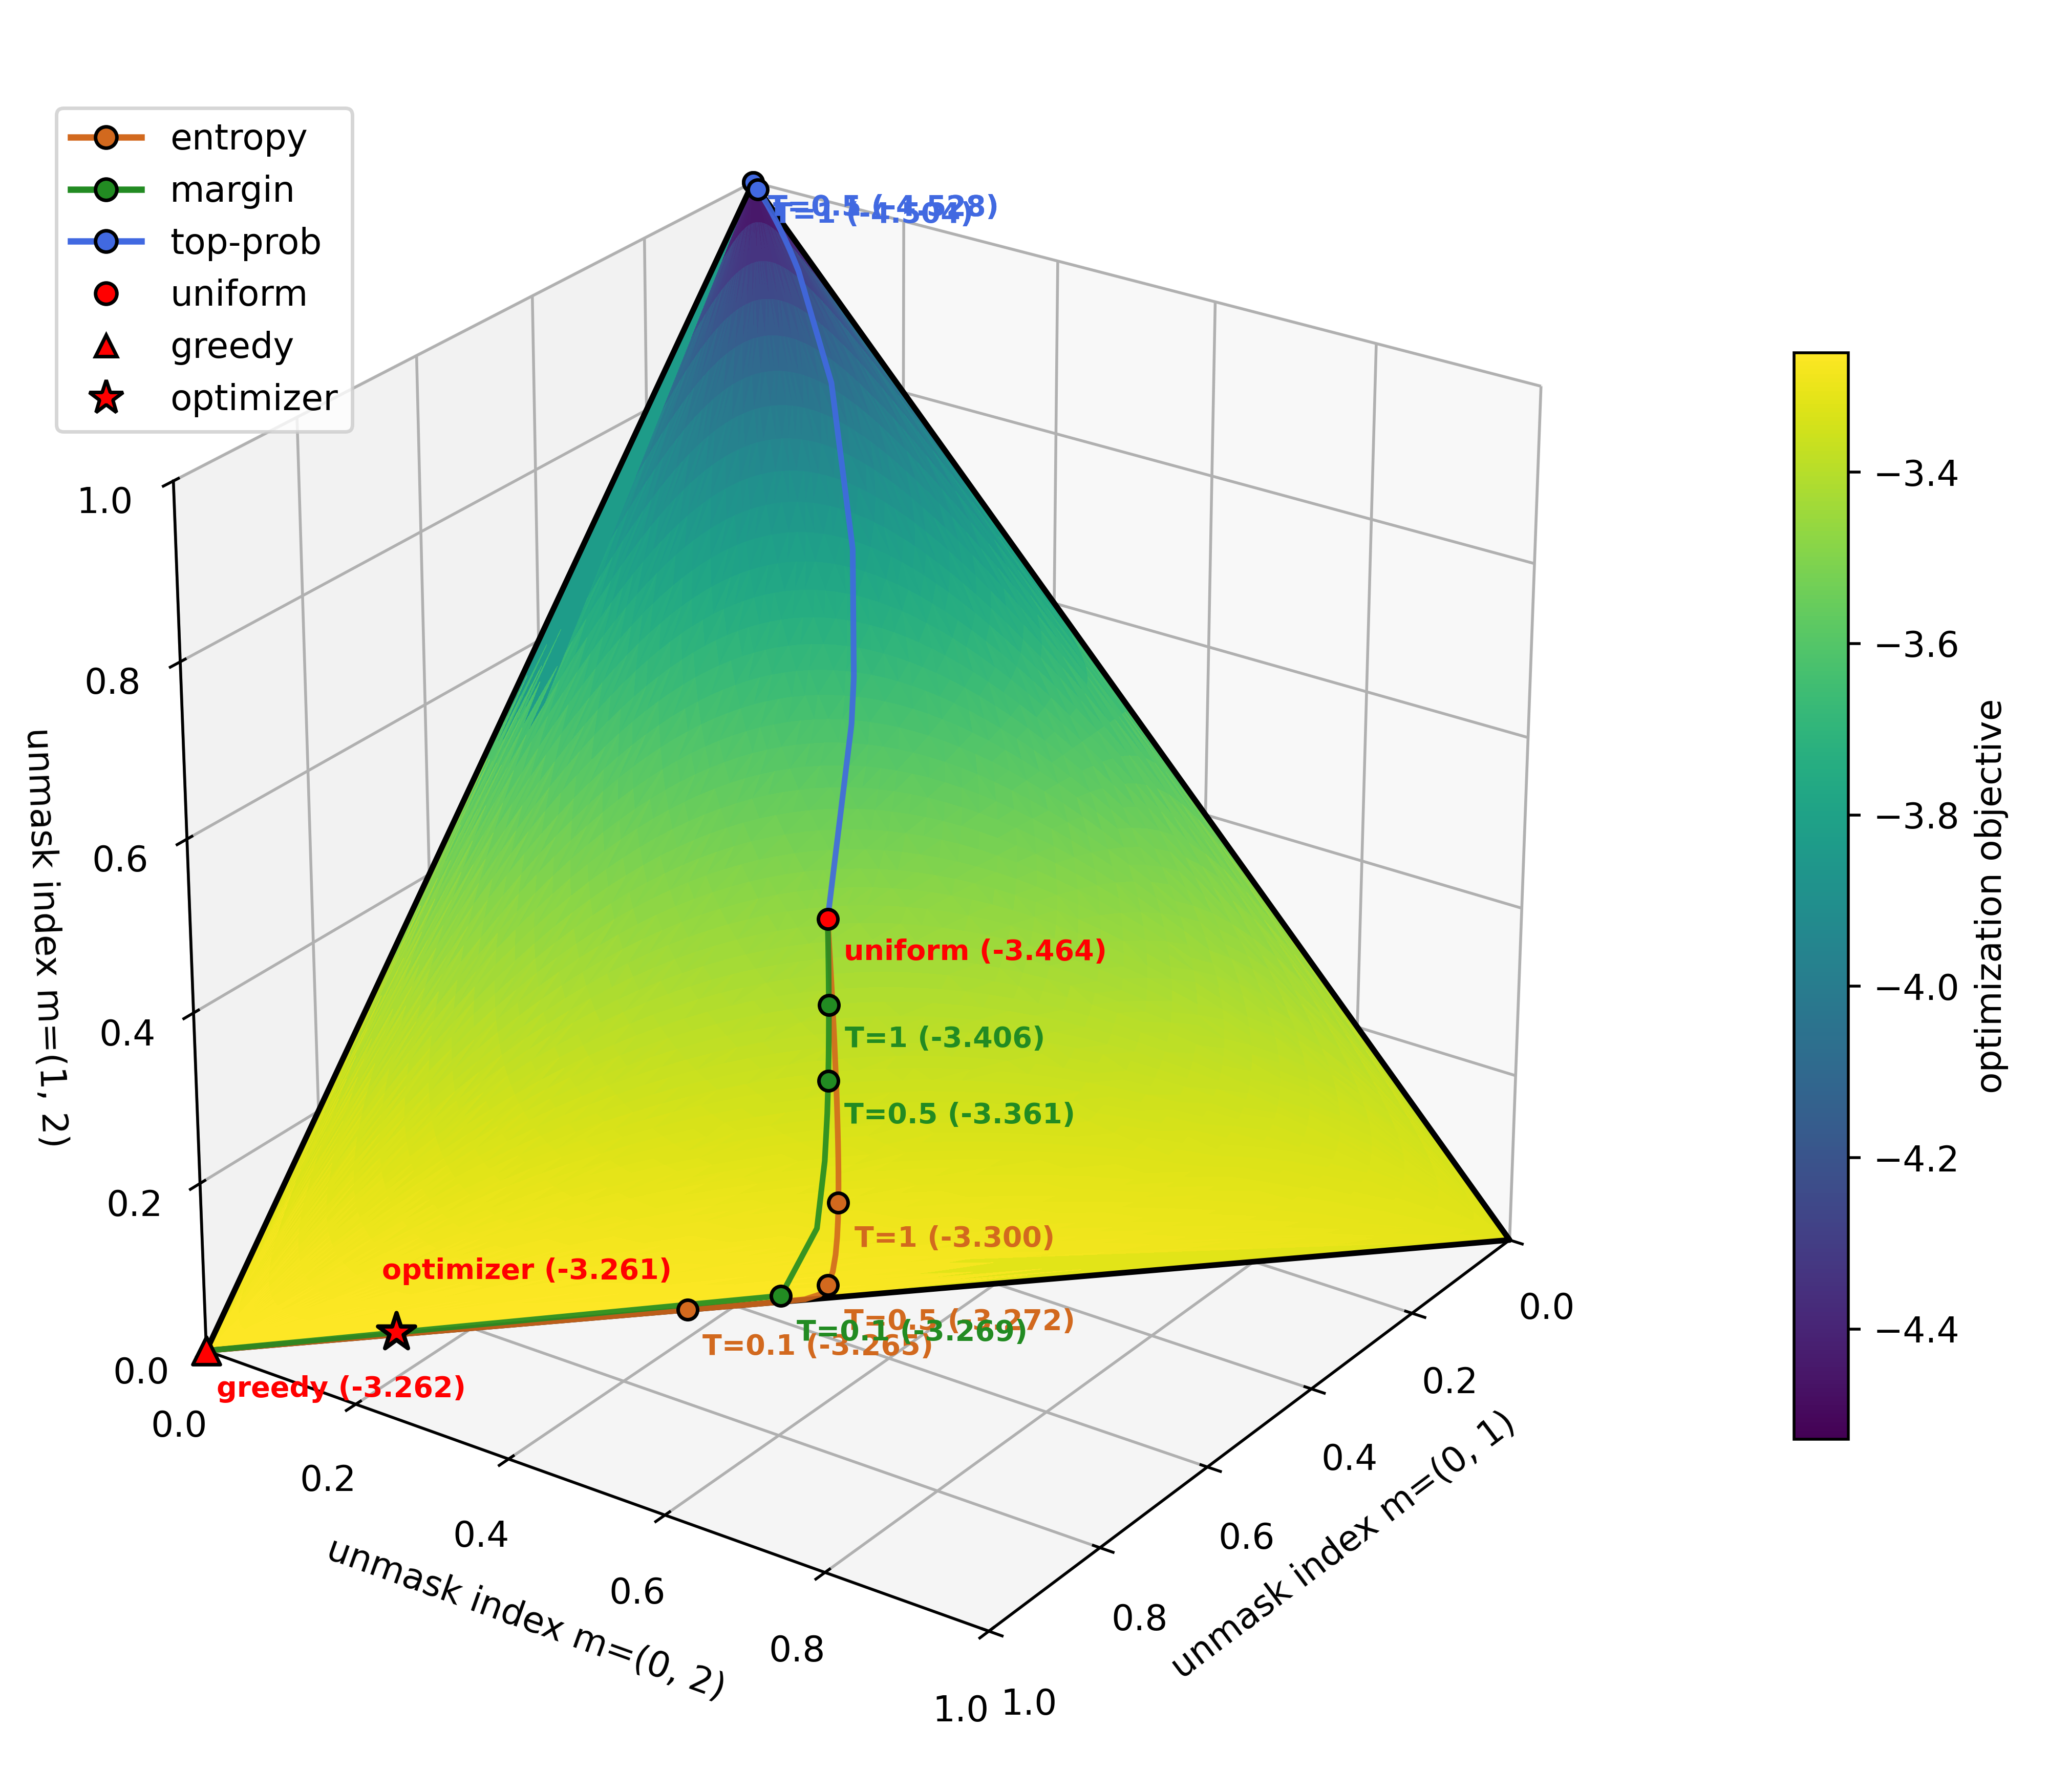
\includegraphics[width=\linewidth]{figs/policy_simplex_seed_6.png}
    \end{subfigure}
    \hfill
    \begin{subfigure}[h]{0.48\linewidth}
        \centering
        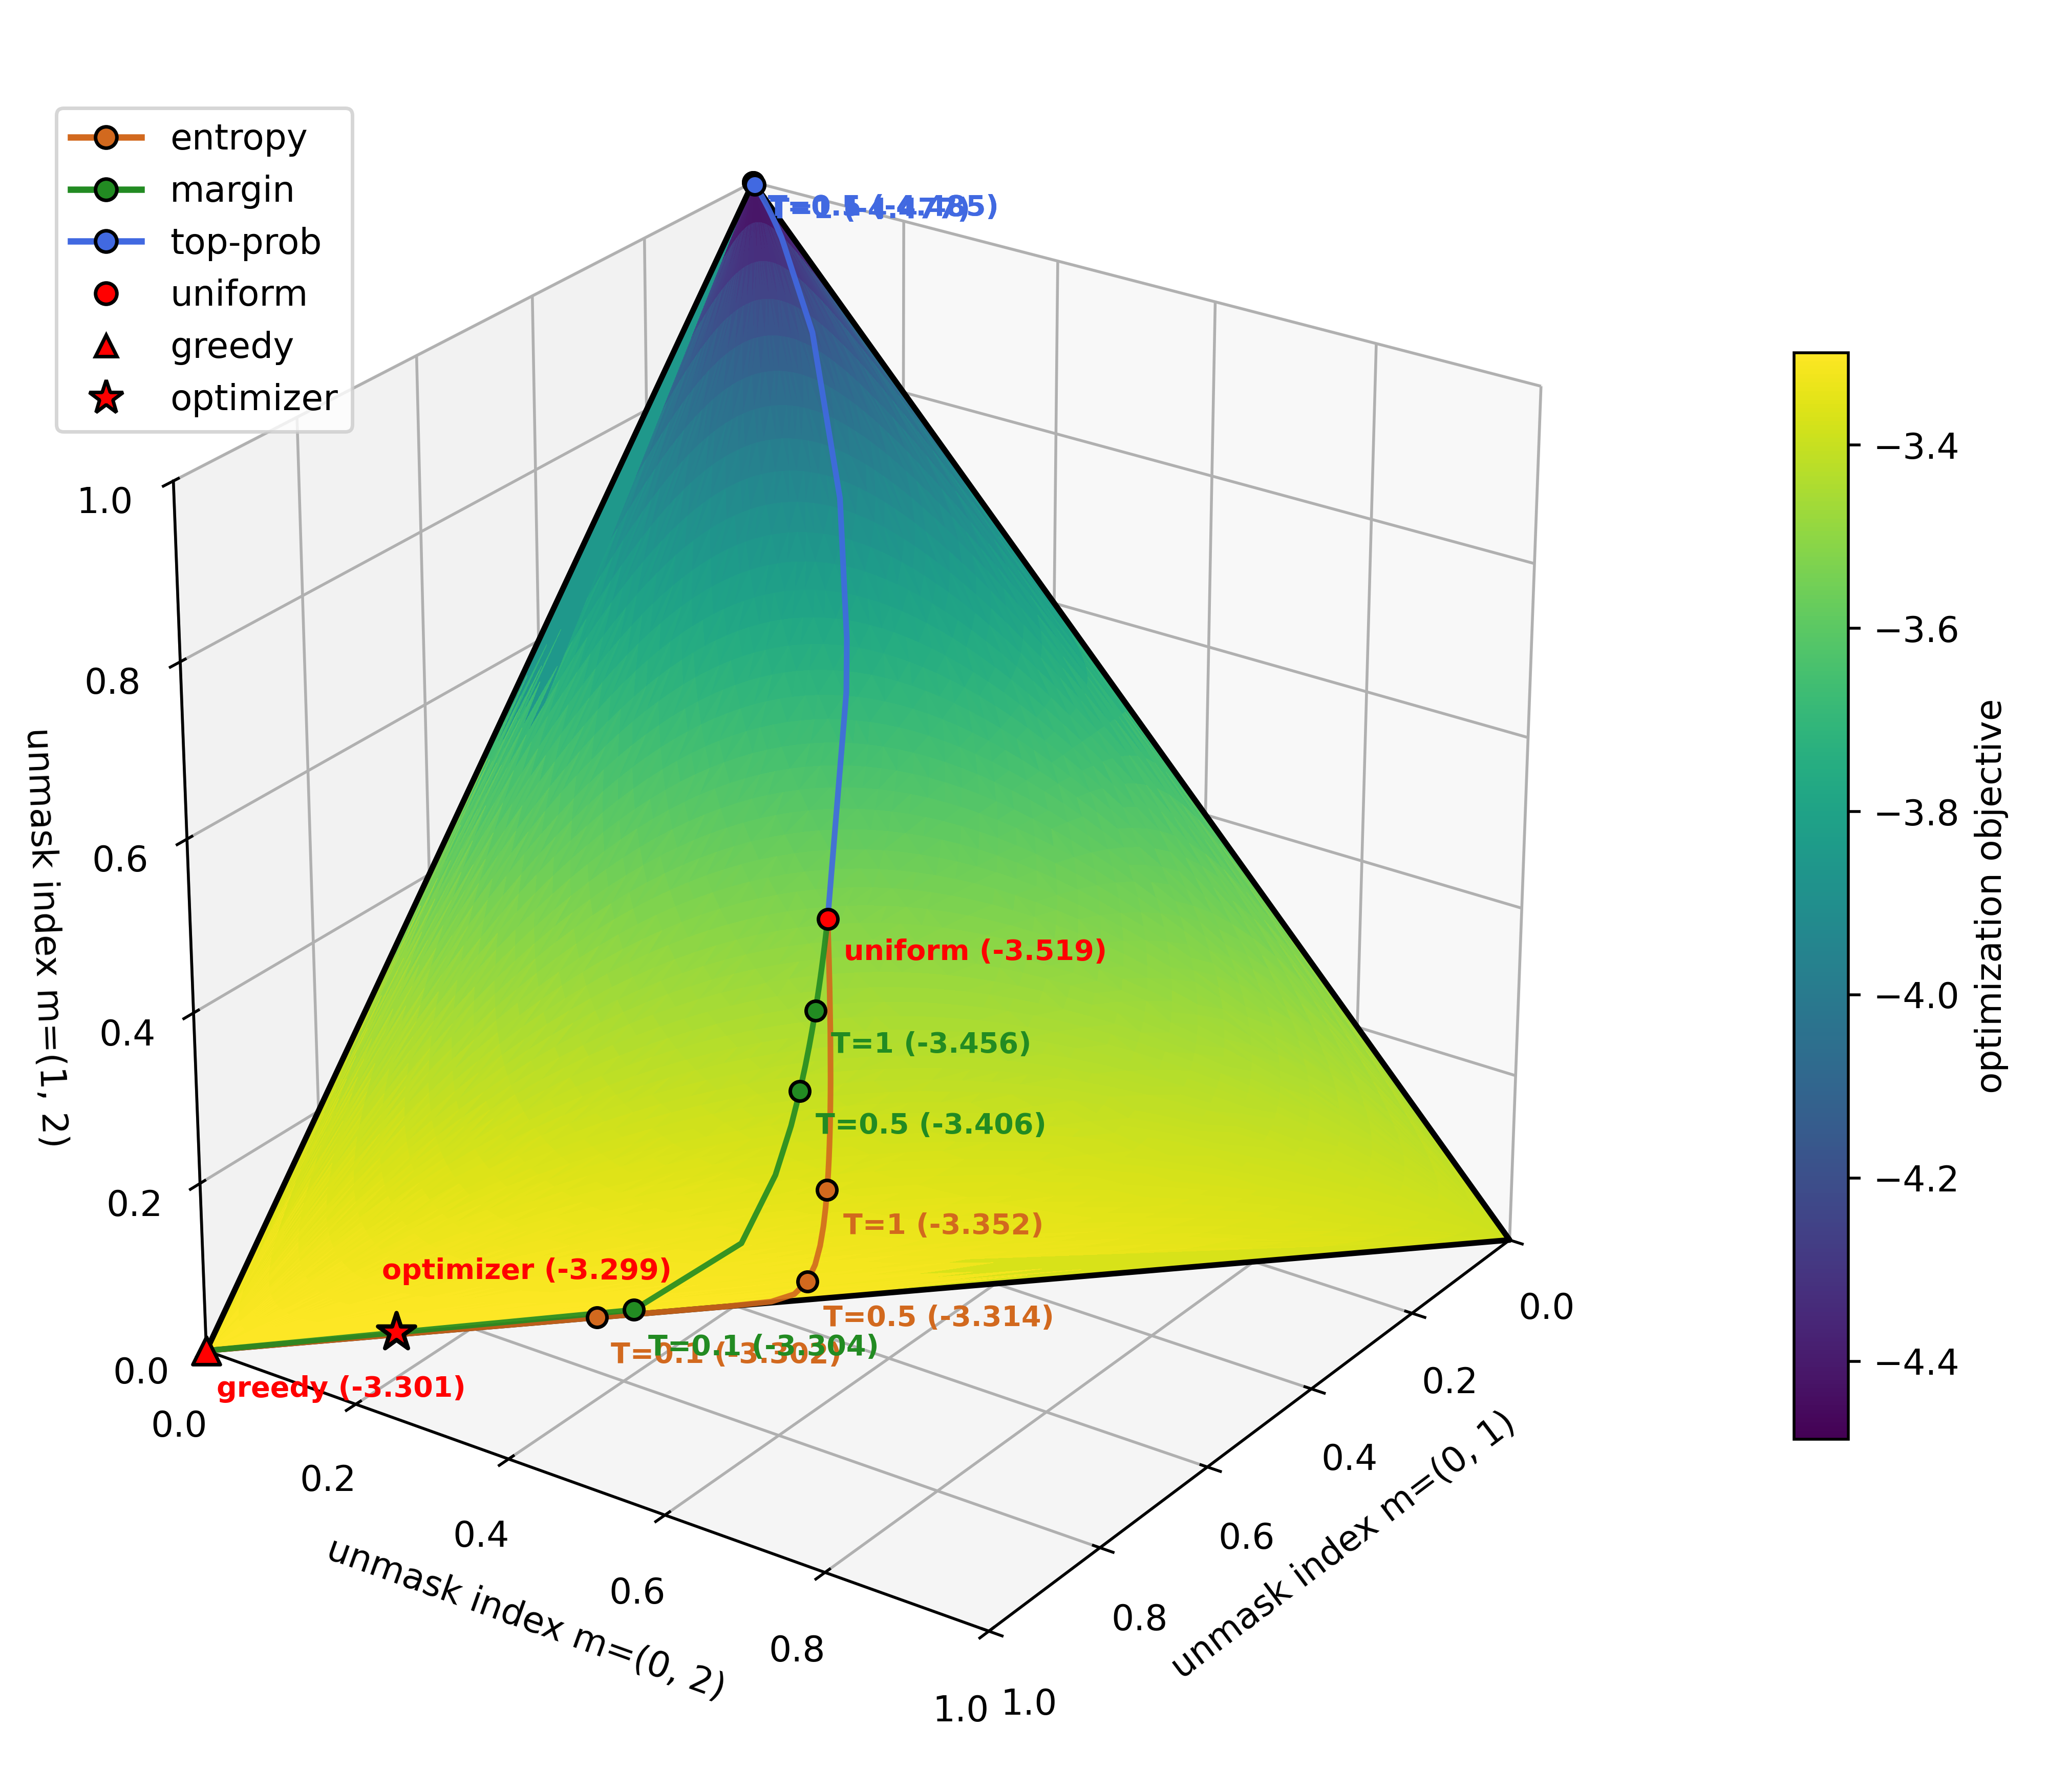
\includegraphics[width=\linewidth]{figs/policy_simplex_seed_8.png}
    \end{subfigure}
    \\
    \begin{subfigure}[h]{0.48\linewidth}
        \centering
        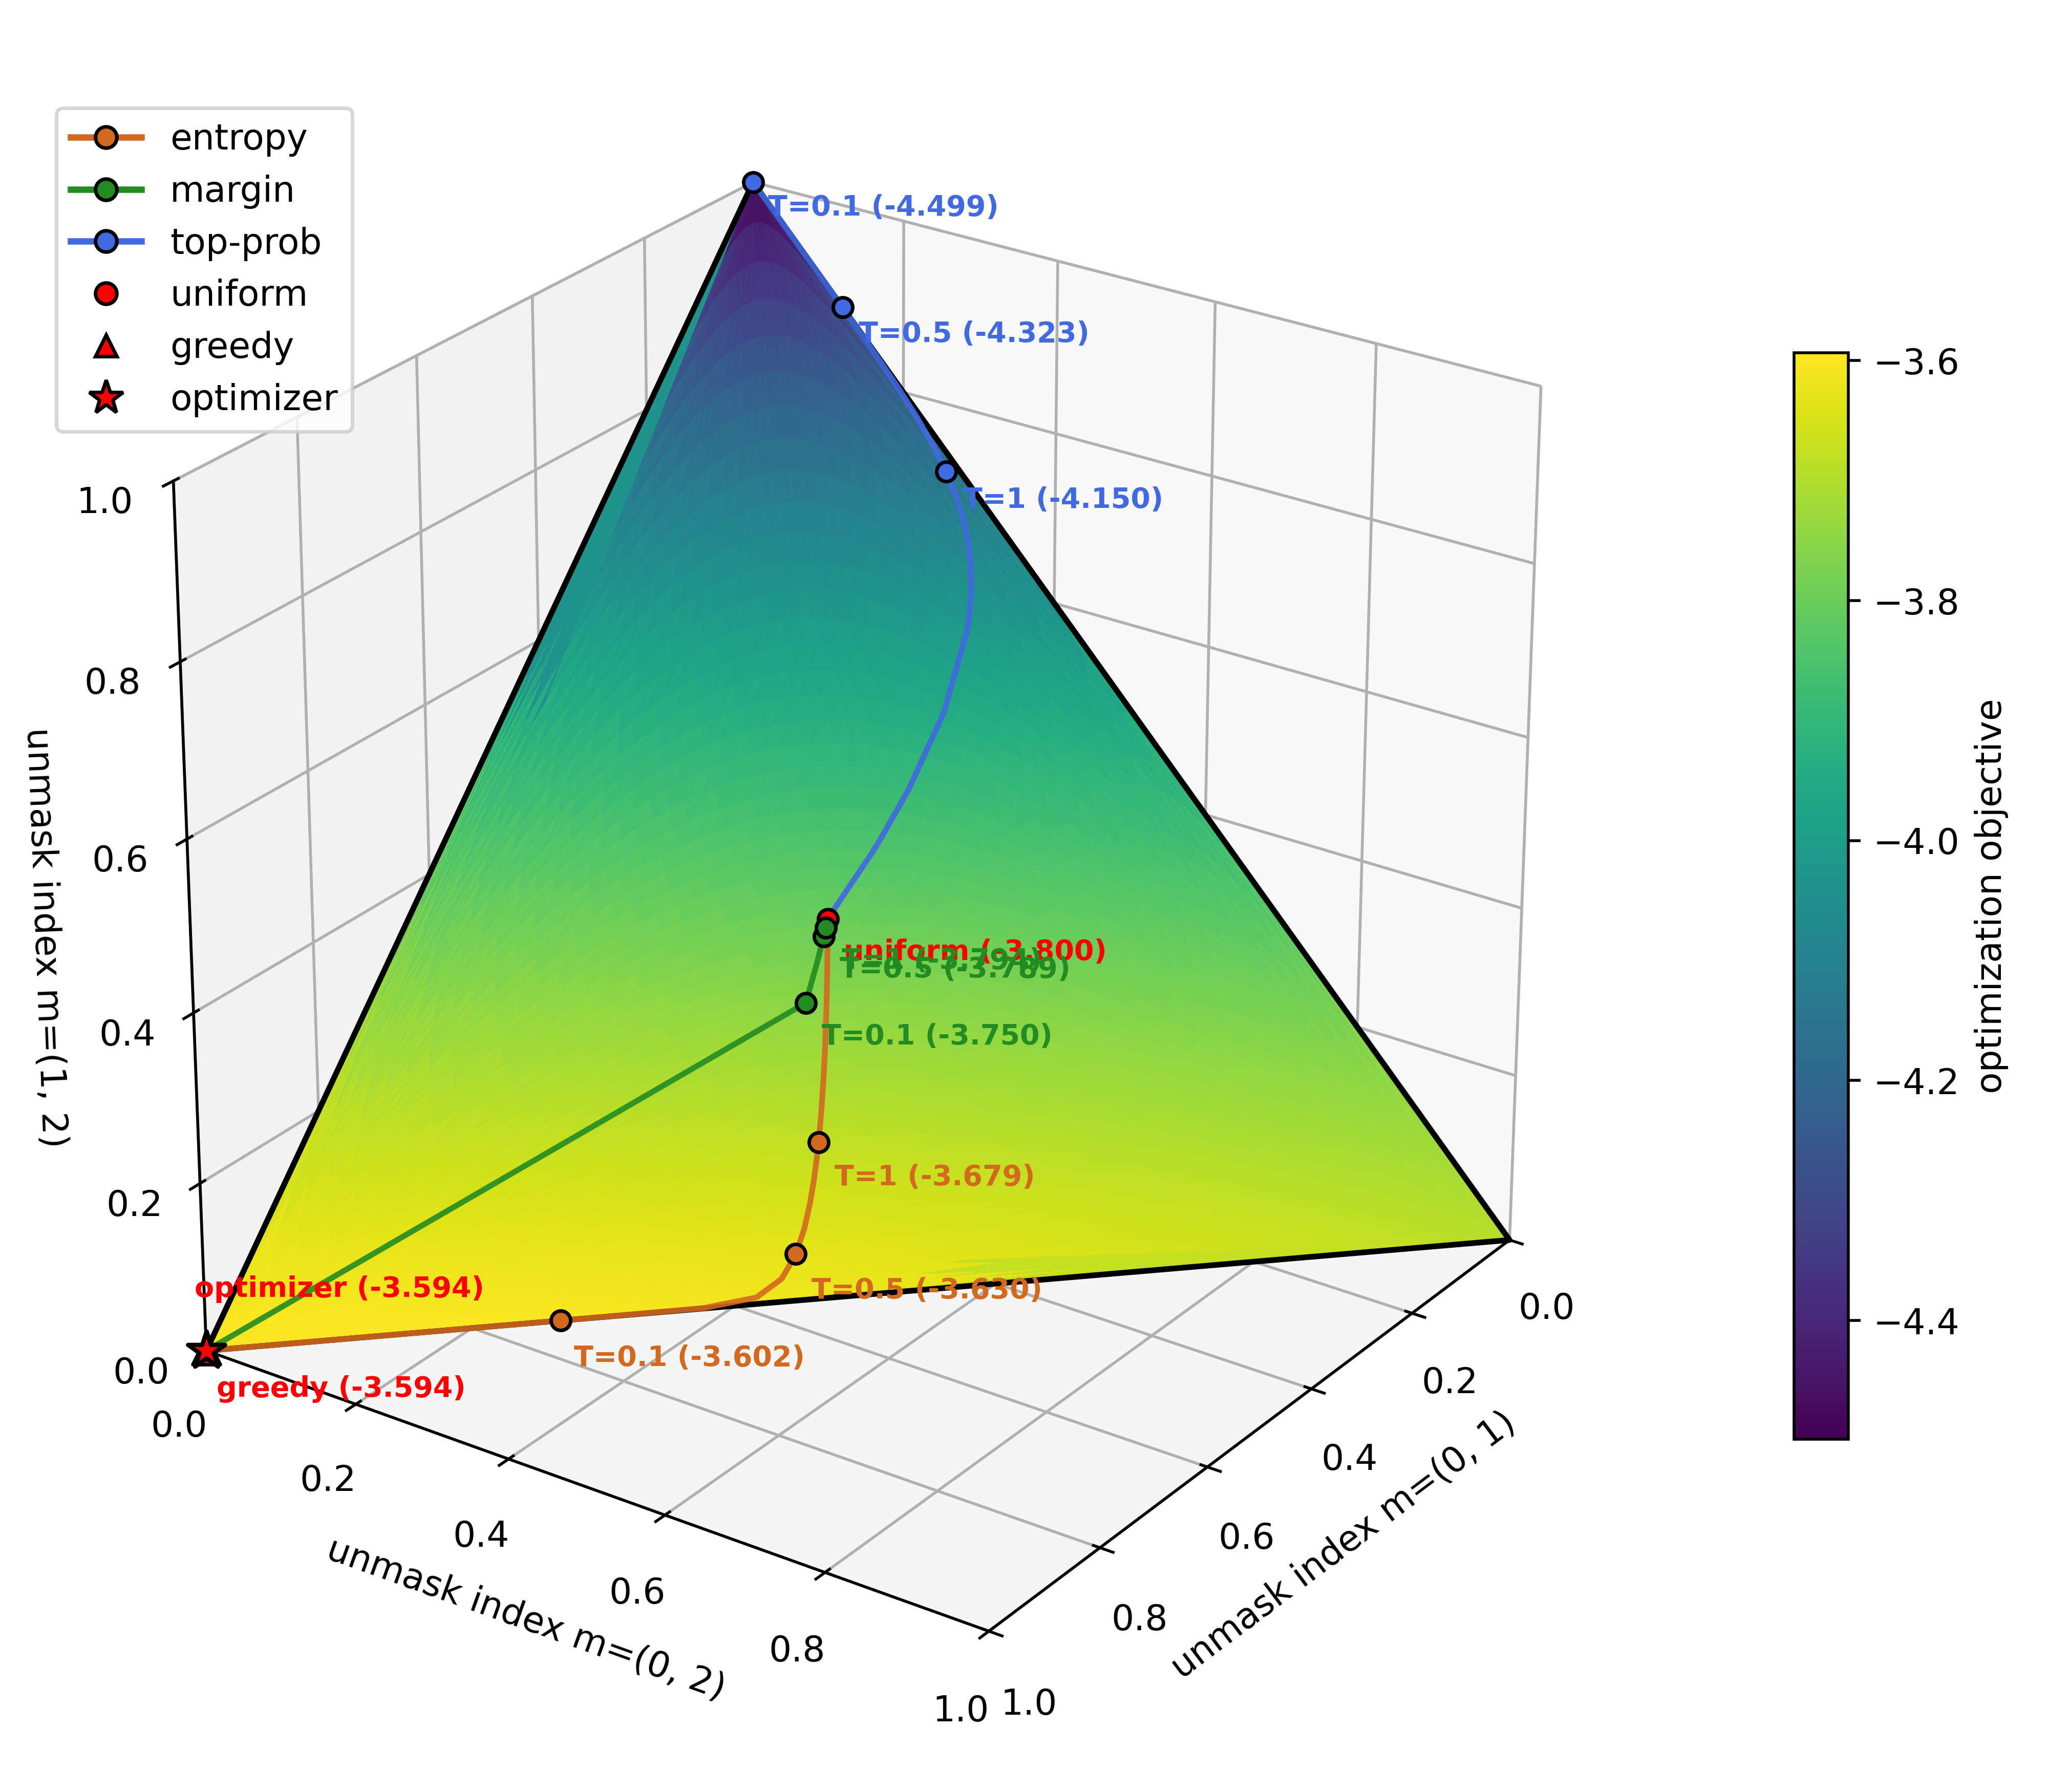
\includegraphics[width=\linewidth]{figs/policy_simplex_seed_10.png}
    \end{subfigure}
    \hfill
    \begin{subfigure}[h]{0.48\linewidth}
        \centering
        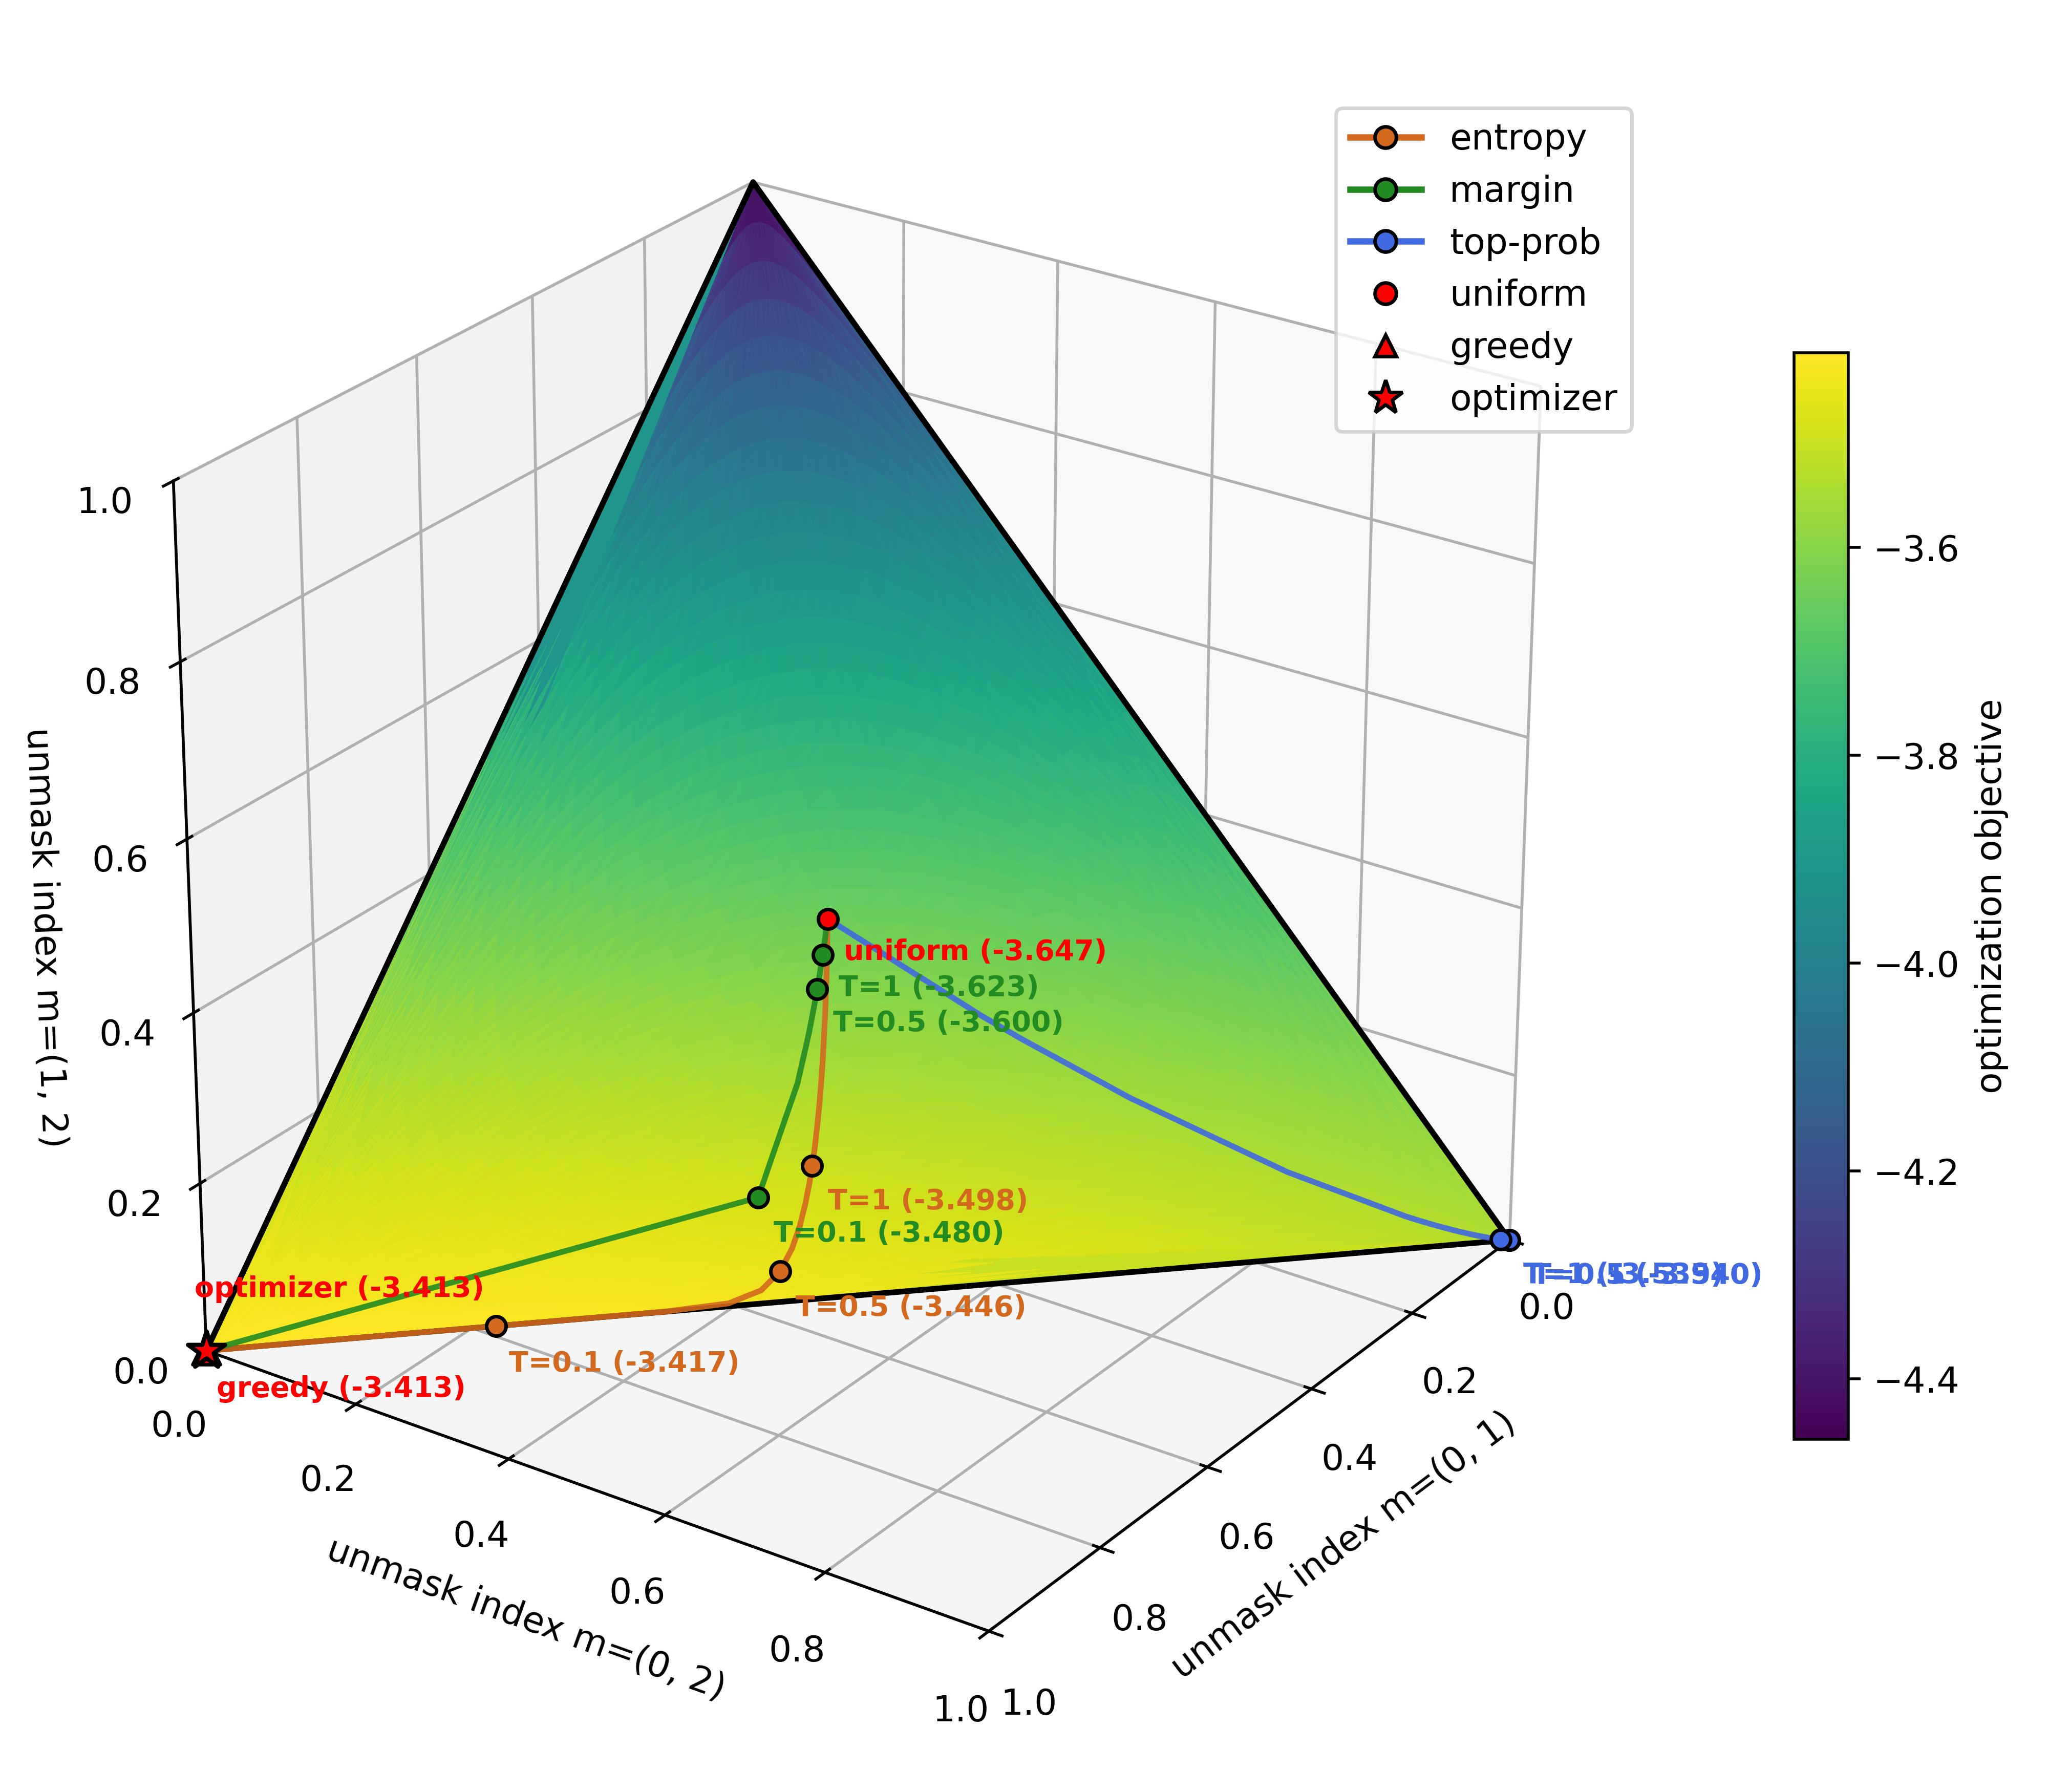
\includegraphics[width=\linewidth]{figs/policy_simplex_seed_12.png}
    \end{subfigure}
    \caption{Policy simplex and different unmasking strategies under various choices of data-generating seed in the synthetic data.}
    \label{fig:policy-simplex-seed}
\end{figure}

\subsubsection{Text Generation Experiments}\label{subsec:radd-gen-exp}

We evaluate the objective value induced by different unmasking strategies during diffusion-based text generation. 
Samples are generated using the pretrained RADD model \citep{ou2024your}. The generation length is fixed to 1024 tokens with batch size 4, and each experiment is repeated over 100 independent sampling runs. 
We vary the number of sampling steps \(N \in \{128,256,512,1024\}\). 
At each sampling step \(i\), the sampler unmasks \(1024/N\) token positions. We compare three strategies: uniform unmasking, greedy confidence based on top-2 probability margin, and its randomized version.

For each run and sampling step, we estimate the objective value \eqref{eq:trainable_confidence} using Monte Carlo approximation. 
Given the model conditional token distribution at the current partially masked sequence, we sample complete token proposals and random unmasking subsets. 
The objective is estimated from the log probability of selecting the subset together with the conditional token likelihood, with a combinatorial correction for the number of possible subsets. 
In the implementation, we use 10 Monte Carlo token samples and 10 sampled unmasking subsets per step. 
For the greedy case, the objective is computed using the top selected negative-entropy terms. 

For each \(N\), we aggregate the objective values across up to 100 runs for each strategy in Figure~\ref{fig:radd-obj-all-step}. Faint curves display the raw per-run objective trajectories, while solid curves show the mean objective value at each sampling step.

\begin{figure}[h]
    \centering
    \begin{subfigure}[h]{0.48\linewidth}
        \centering
        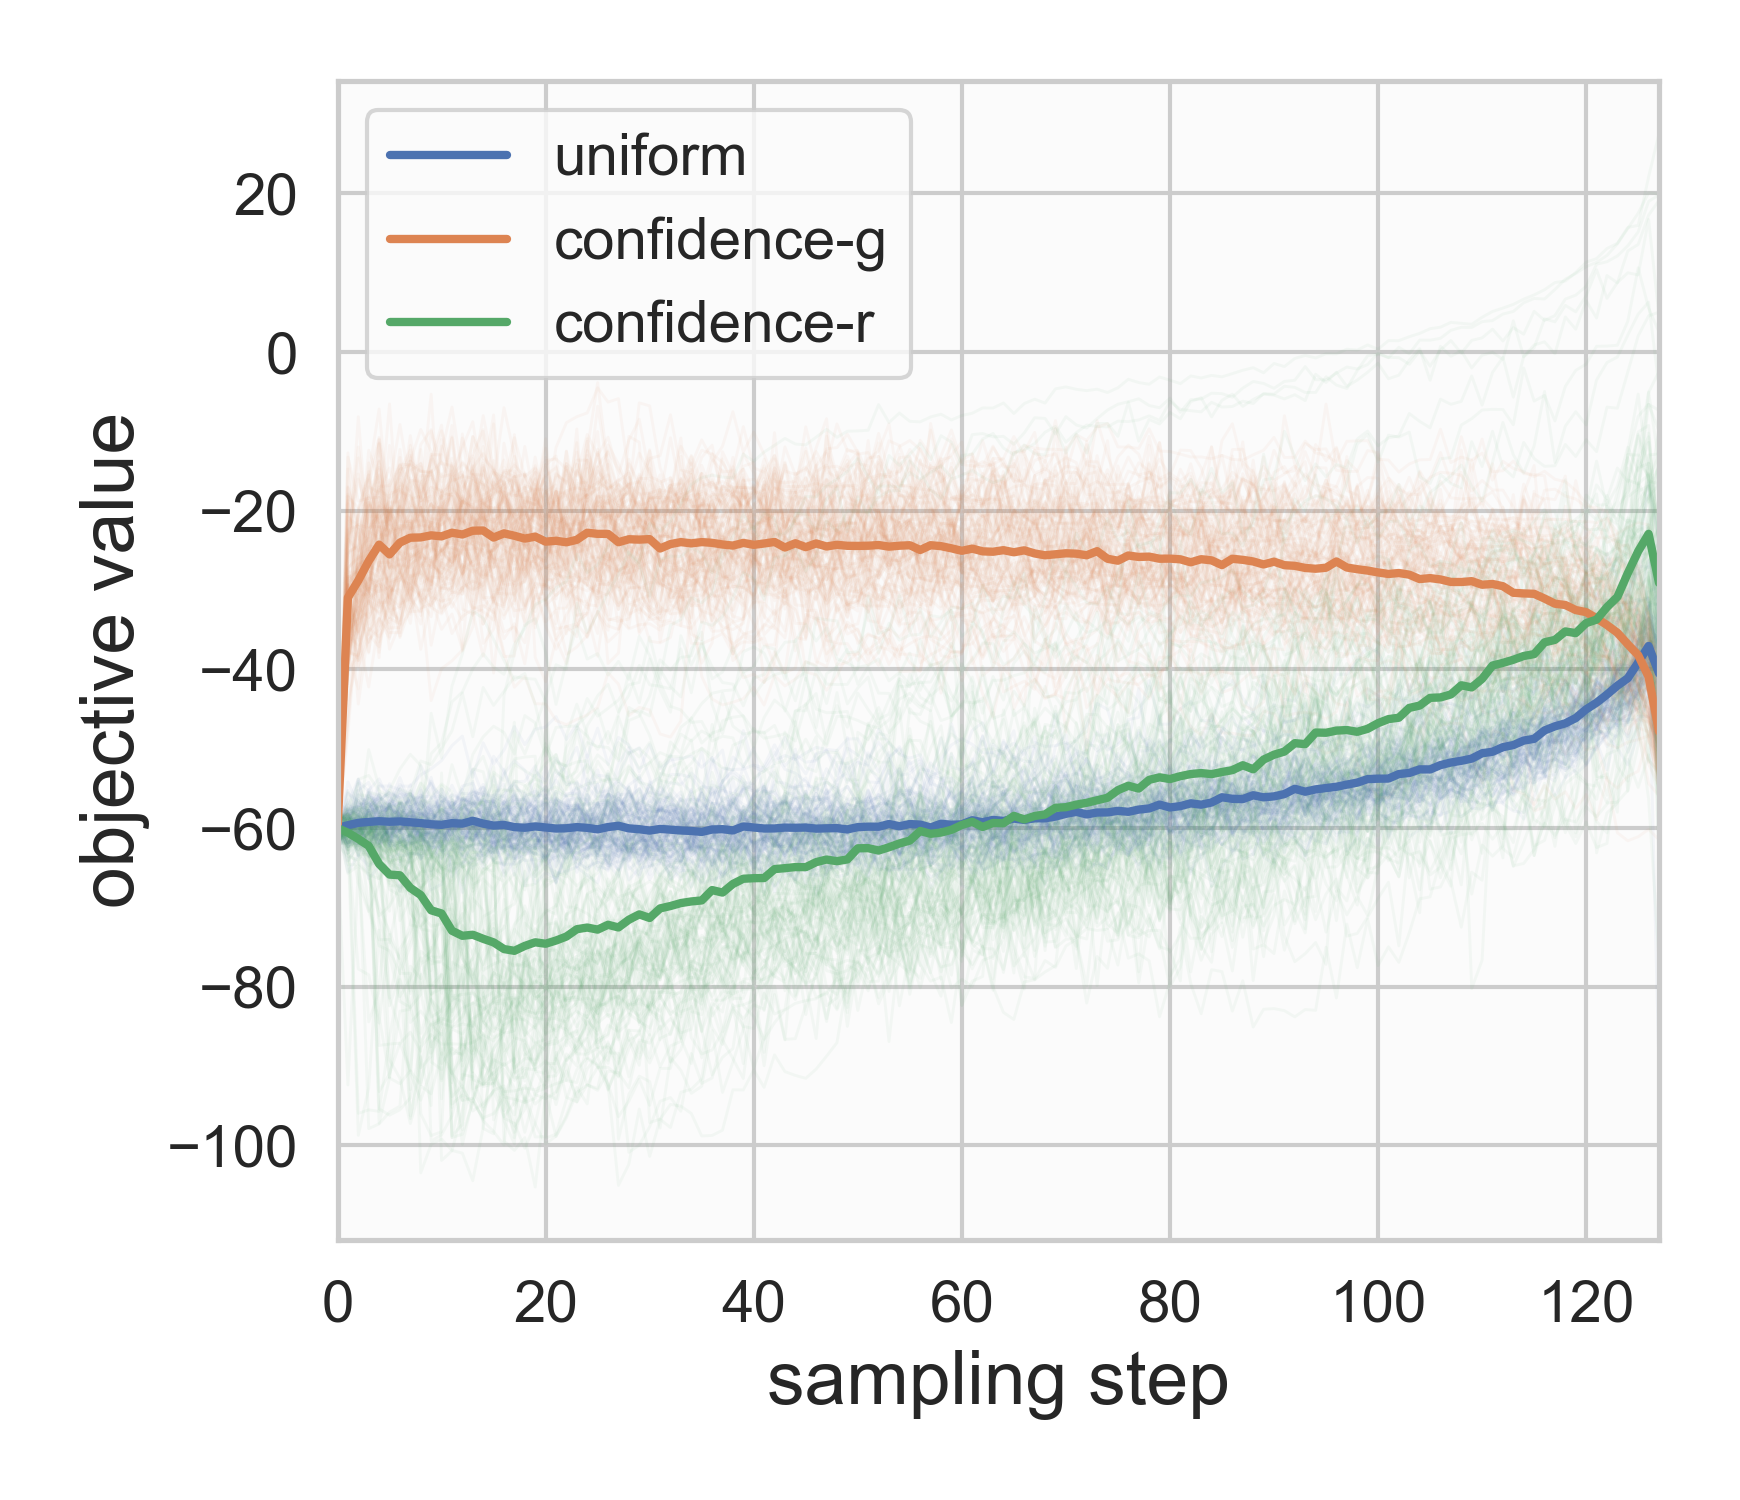
\includegraphics[width=\linewidth]{figs/objective_steps_128.png}
        \caption{128 steps}
    \end{subfigure}
    \hfill
    \begin{subfigure}[h]{0.48\linewidth}
        \centering
        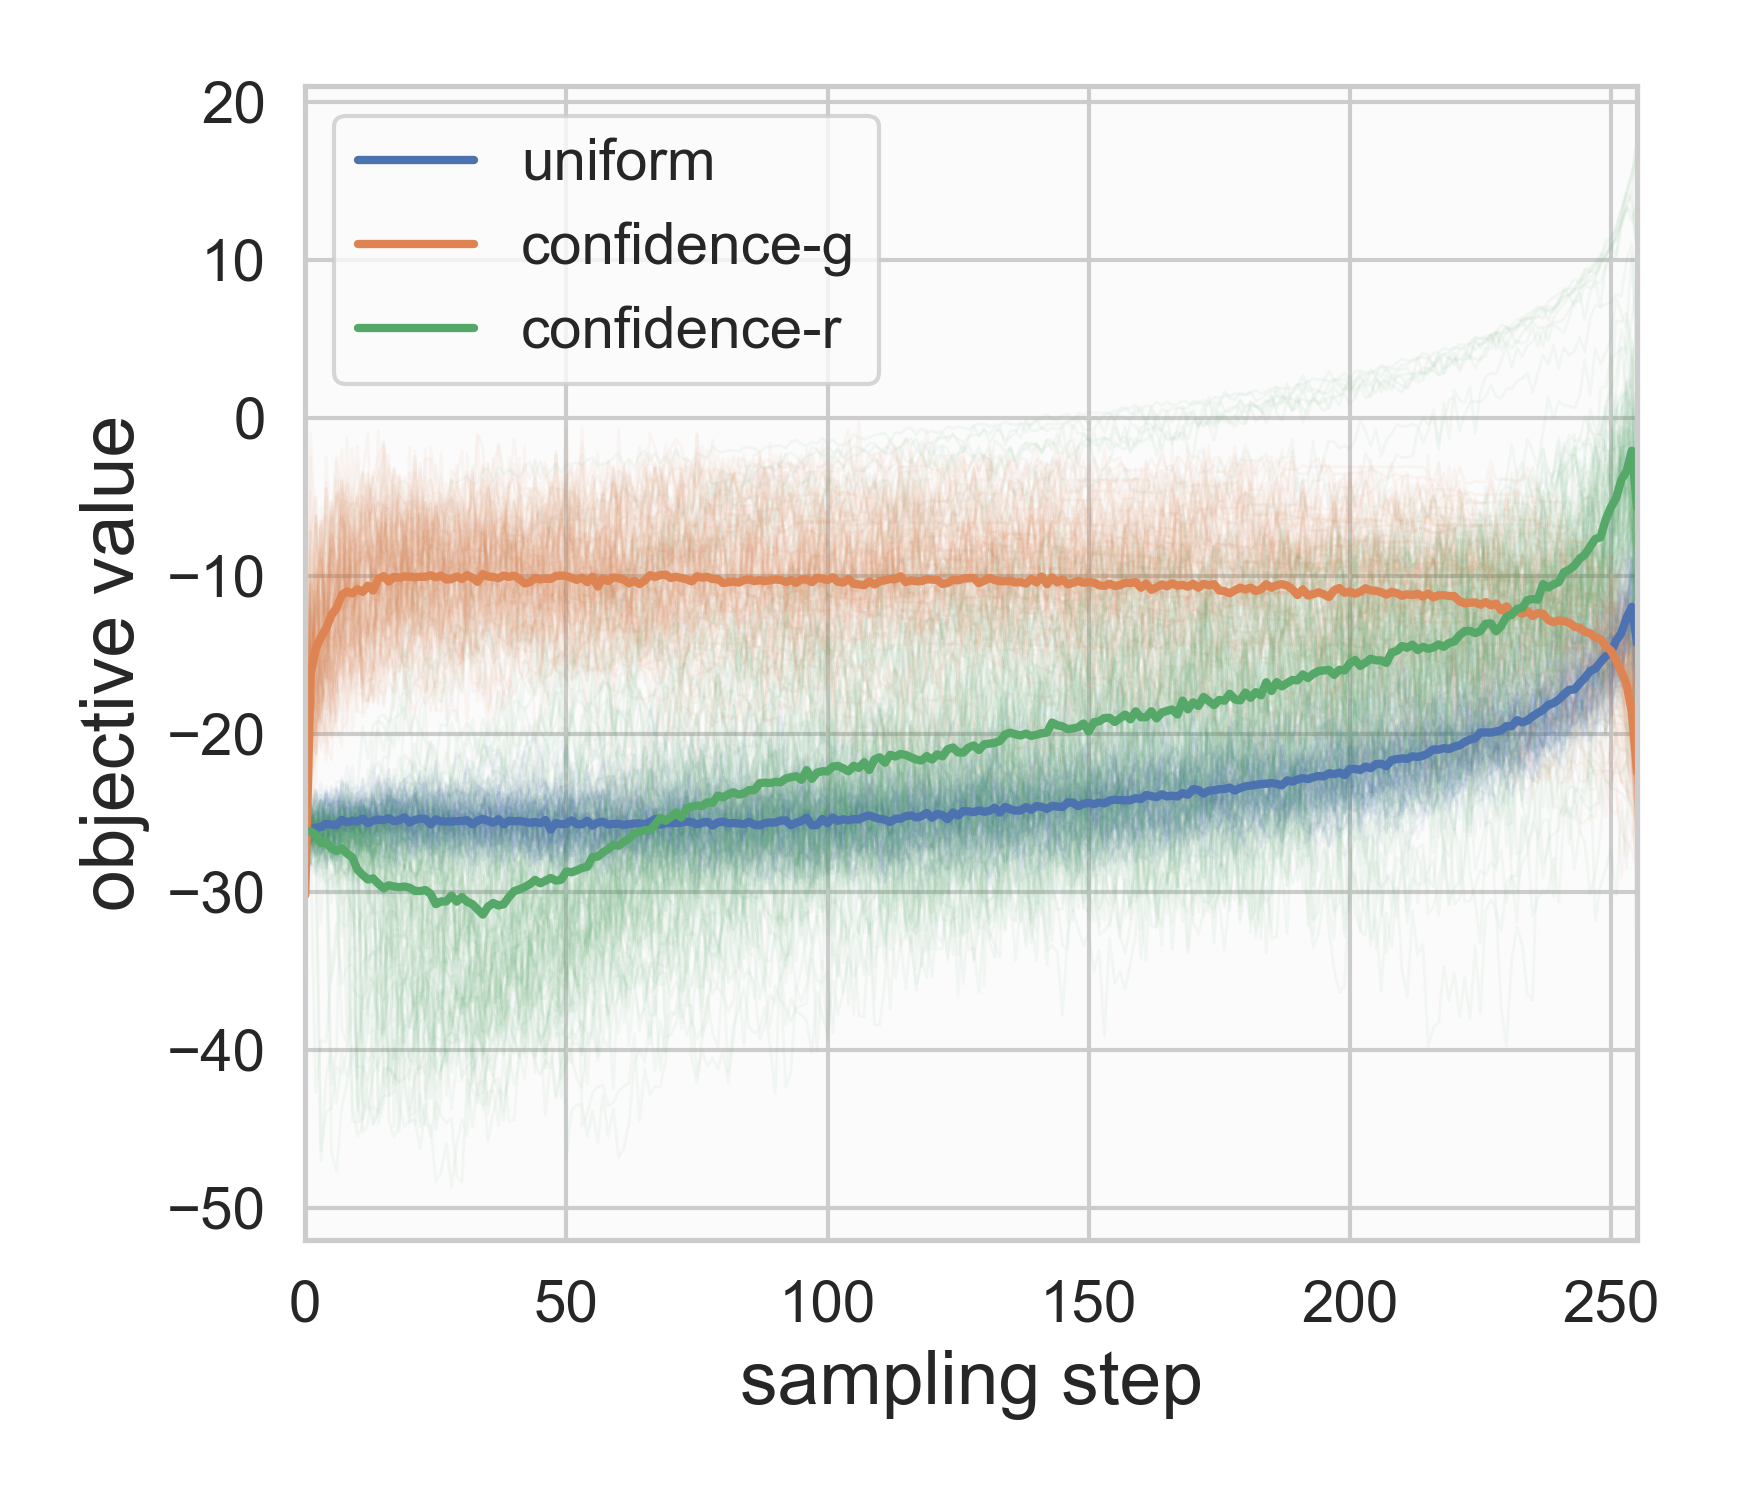
\includegraphics[width=\linewidth]{figs/objective_steps_256.png}
        \caption{256 steps}
    \end{subfigure}
    \\
    \begin{subfigure}[h]{0.48\linewidth}
        \centering
        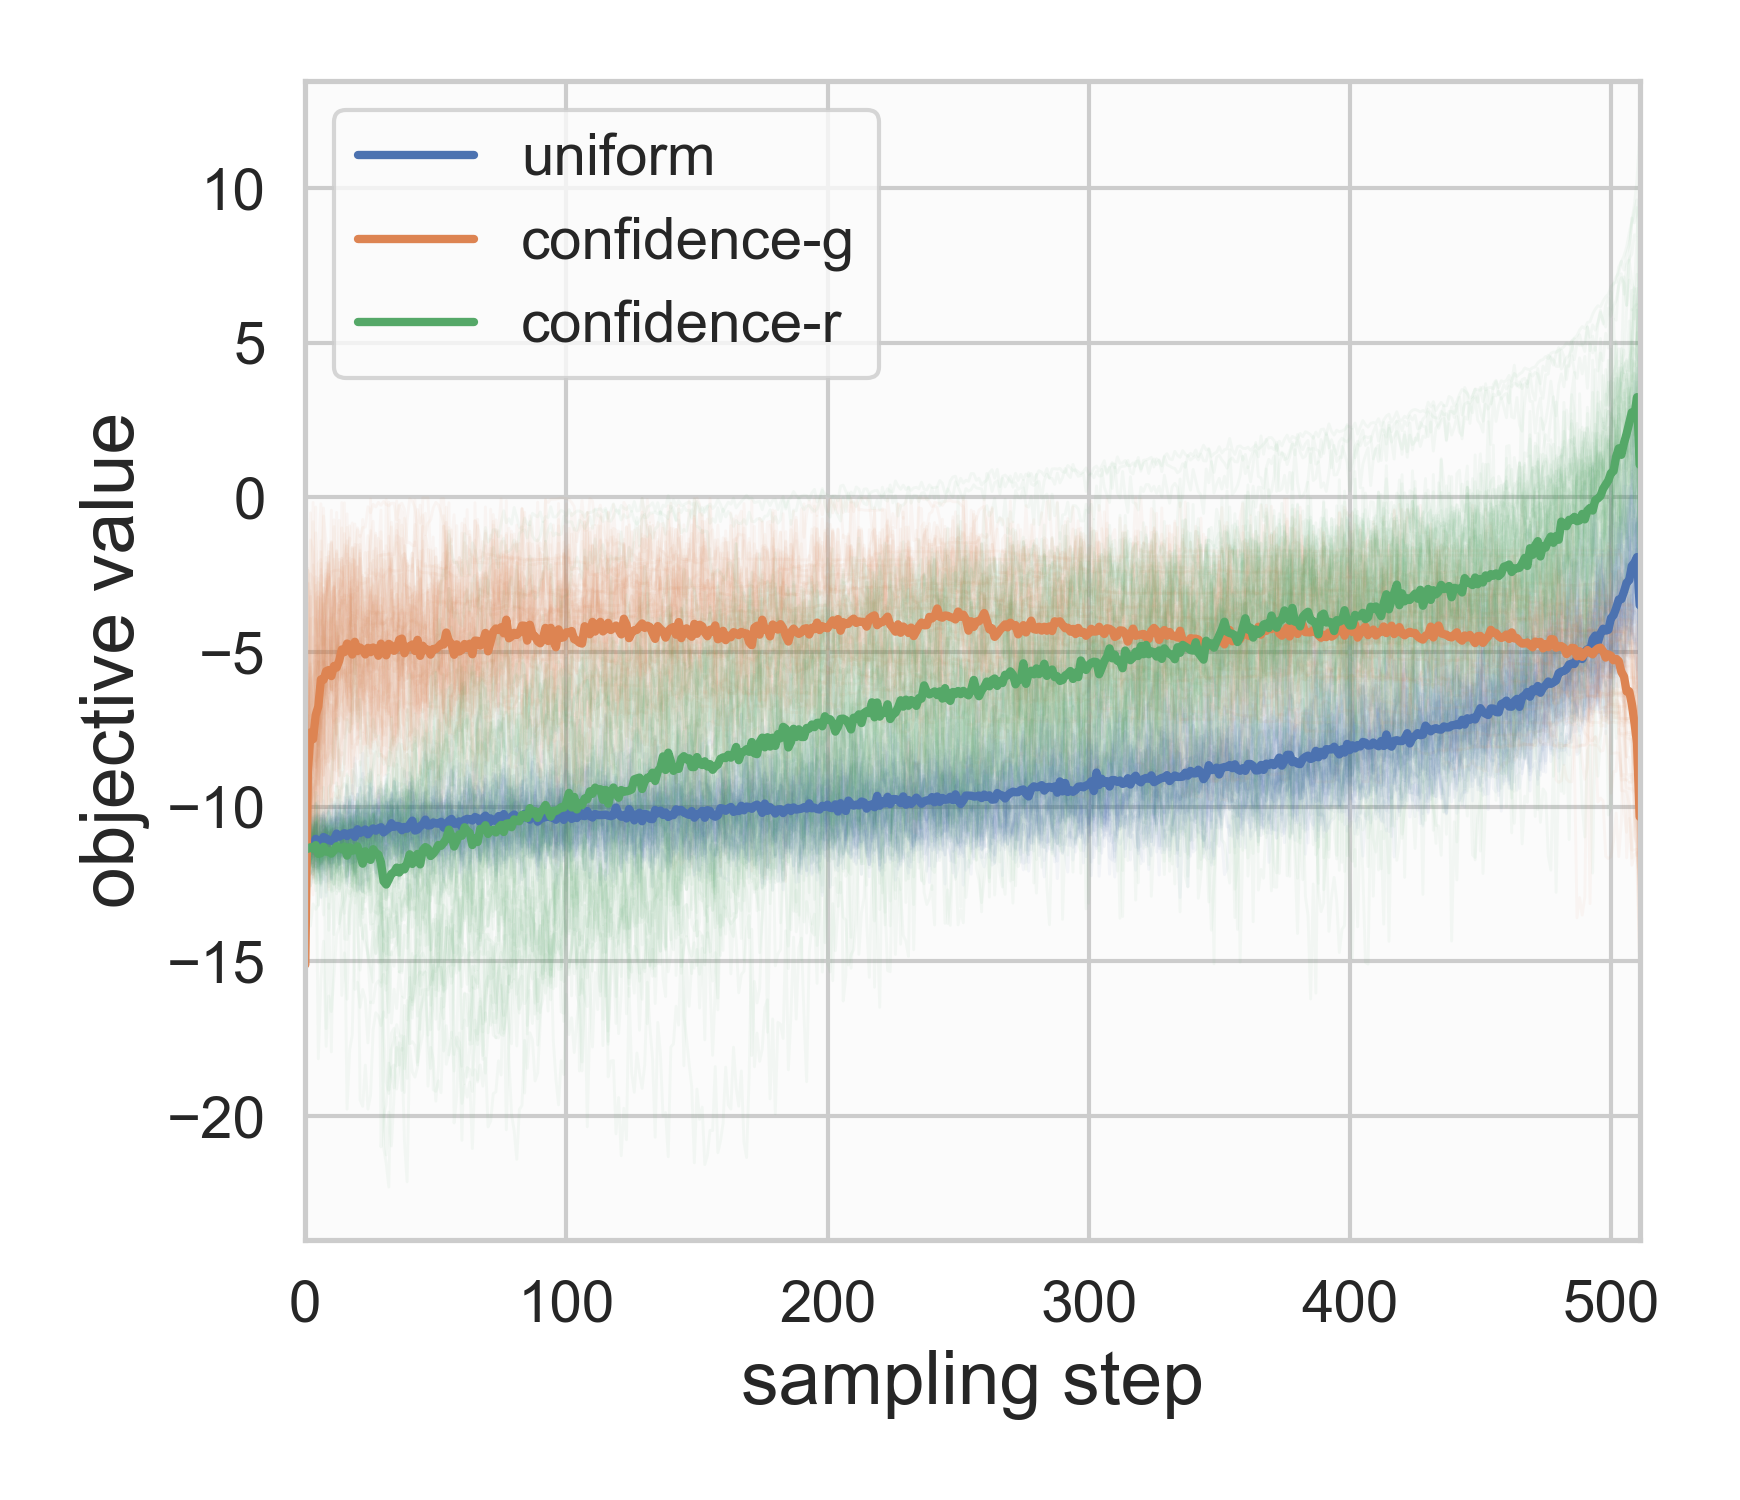
\includegraphics[width=\linewidth]{figs/objective_steps_512.png}
        \caption{512 steps}
    \end{subfigure}
    \hfill
    \begin{subfigure}[h]{0.48\linewidth}
        \centering
        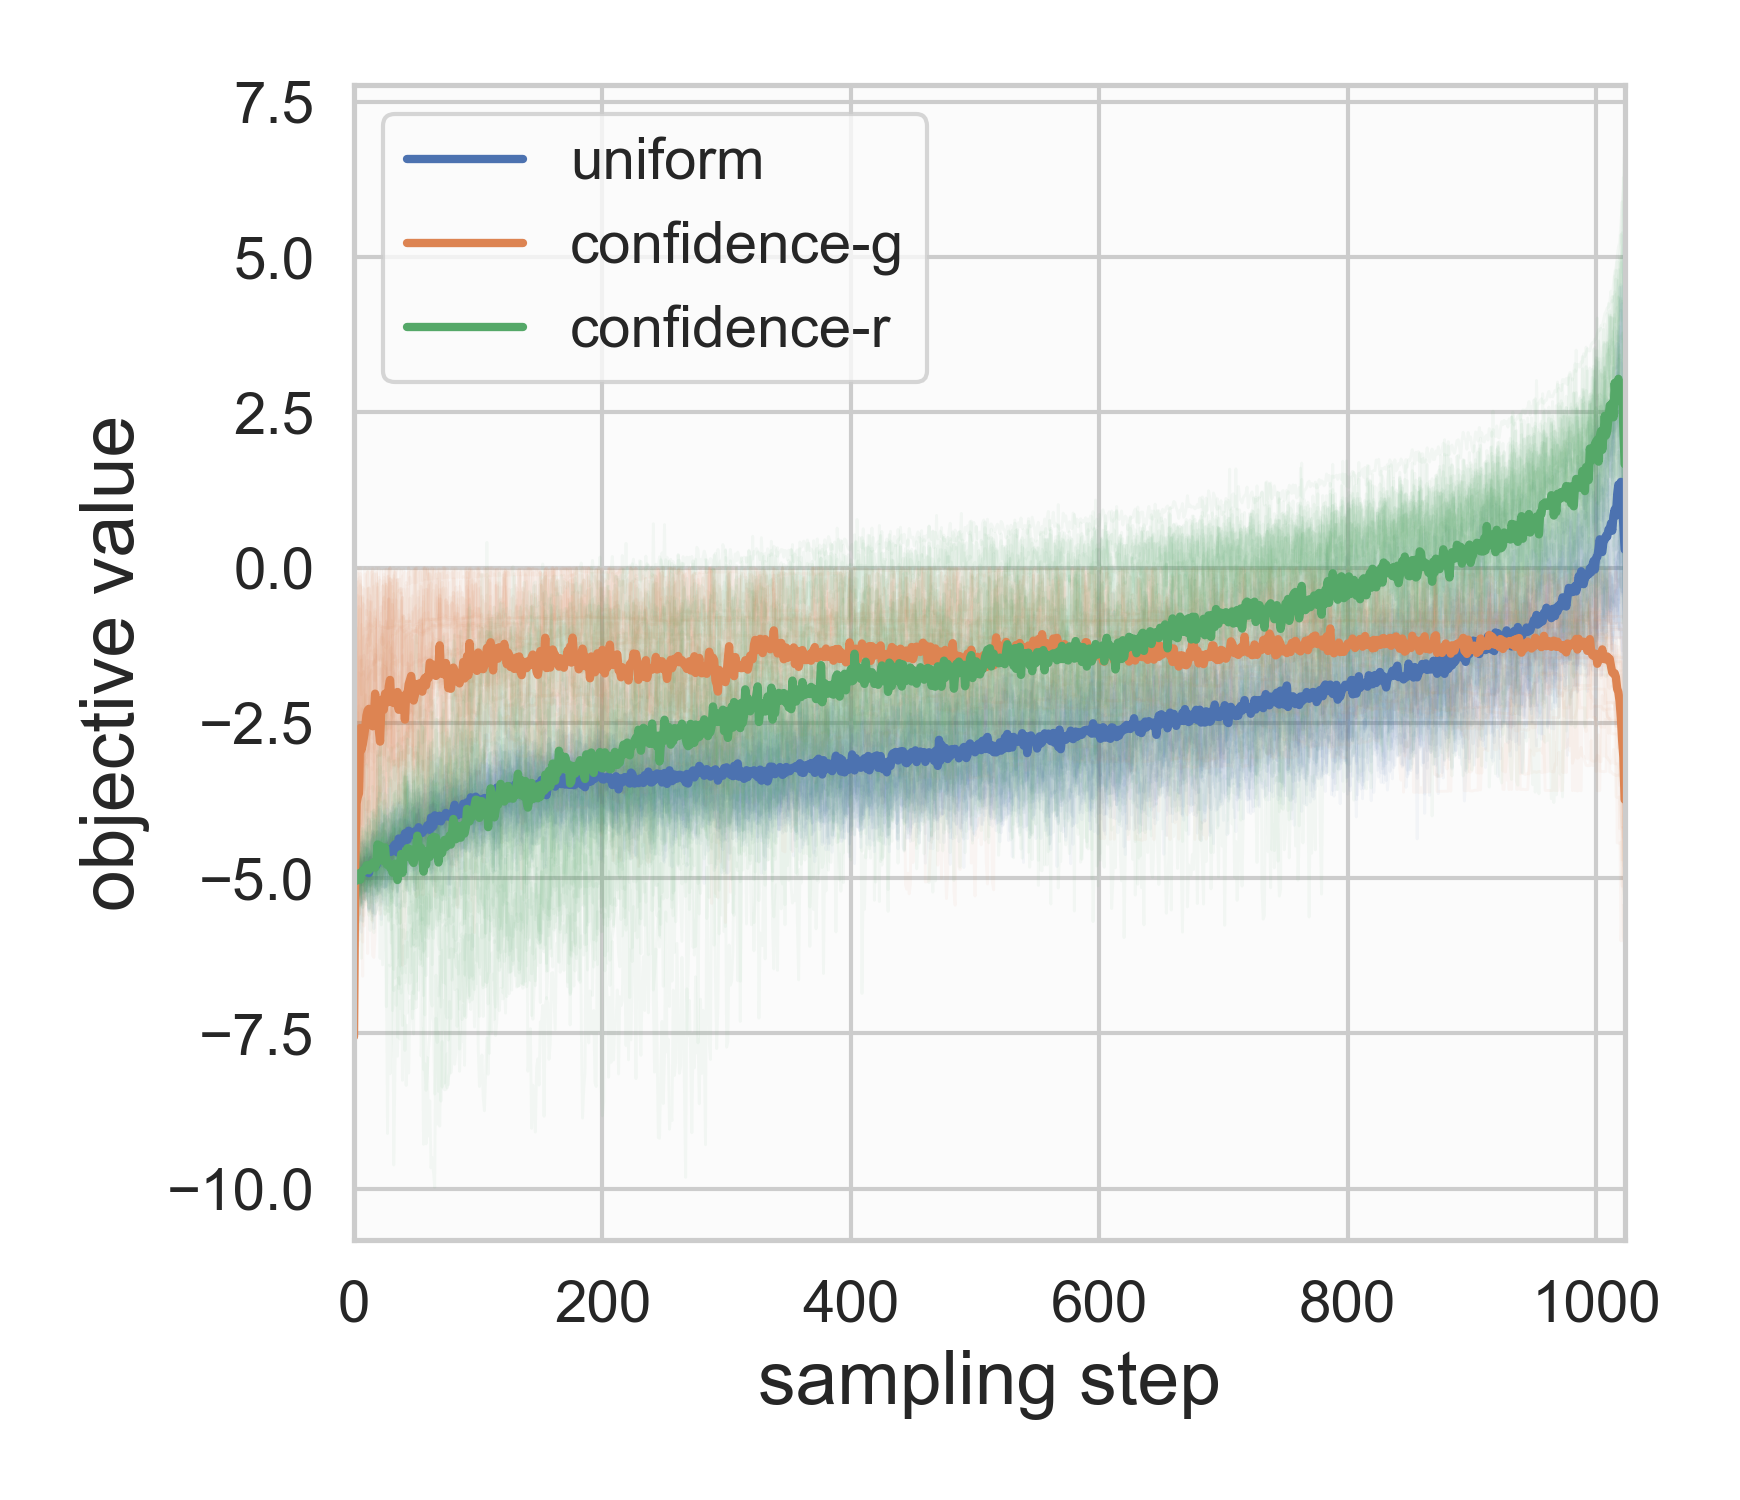
\includegraphics[width=\linewidth]{figs/objective_steps_1024.png}
        \caption{1024 steps}
    \end{subfigure}
    \caption{Local objective values \eqref{eq:trainable_confidence} attained by different unmasking methods in text generation with RADD~\citep{ou2025absorbingdiscretediffusionsecretly}.}
    \label{fig:radd-obj-all-step}
\end{figure}

\subsection{Evaluation of VLP}\label{sec:vlp}

\subsubsection{Experiment Setup}\label{sec:vlp-experiment-setup}

\paragraph{Text Generation Details.}

For the RADD text generation experiments, we use the pretrained checkpoint corresponding to the small RADD configuration with 12 Transformer blocks, hidden size 768, 12 attention heads, sequence length 1024, and approximately 162M parameters. The backbone is kept frozen throughout policy training. The policy network follows Section~\ref{subsec:architecture}, with approximately 5.3M trainable parameters, about 3\% of the RADD backbone.

We train the policy on OpenWebText. Text is tokenized with the GPT-2 tokenizer, appended with EOS tokens, concatenated, and split into fixed-length chunks of 1024 tokens. Since this is unconditional generation, there is no prompt portion and all positions are eligible for masking or unmasking. Unless otherwise specified, policy training uses batch size 4, one gradient accumulation step, and \(K=32\) discrete masking steps for the RADD runs used in our reported sampling experiments. We optimize with AdamW using learning rate \(3\times 10^{-4}\), weight decay 0, \((\beta_1,\beta_2)=(0.9,0.999)\), \(\epsilon=10^{-8}\), gradient clipping at norm 1.0, and EMA decay 0.9999 for the policy parameters. The KL regularization parameter $\lambda$ is set to $10^{-2}$. Training is run on a single A100 80GB GPU for $2\times10^3$ steps.

For evaluation, we generate unconditional sequences of length 1024 using the RADD diffusion sampler. We evaluate sampling budgets from 16 to 256 steps. For each setting, we generate 100 independent samples and report the mean and standard deviation of GPT-2-large perplexity. We compare uniform unmasking, greedy margin-based confidence unmasking, randomized margin-based confidence unmasking, and the learned policy.


\paragraph{Code and Math Generation Details.}

For both 7B models, we evaluate HumanEval~\citep{chen2021evaluatinglargelanguagemodels}, MBPP~\citep{austin2021programsynthesislargelanguage}, GSM8K~\citep{cobbe2021training}, and MATH500~\citep{lightman2023let}. HumanEval and MBPP are evaluated using Pass@1 ($\uparrow$), while GSM8K and MATH500 are evaluated using final-answer accuracy ($\uparrow$). All evaluations are run through the LM Evaluation Harness with our DiffuCoder wrapper.

The policy is trained on instruction-output pairs from OpenCoder-SFT~\citep{Gokaslan2019OpenWeb} and MetaMathQA~\citep{yu2023metamath}. Each example is converted to the chat format shown in Table~\ref{tab:chat-sft}. We tokenize each formatted sequence with the corresponding model tokenizer, truncate or pad to length 1024, and construct a prompt mask marking all tokens before the assistant response. During training and inference, prompt tokens are kept fixed; only response tokens are masked, unmasked, or generated.

The backbone model is loaded in \texttt{bfloat16} and kept frozen throughout policy training. The trained policy is a lightweight transformer policy network as described in Section~\ref{subsec:architecture}, with approximately 115.7M parameters or about 1.5\% of the 7.6B-parameter backbone.

Unless otherwise specified, we train the policy with batch size 4, sequence length 1024, and \(K=16\) discrete masking steps. We optimize the policy with AdamW using learning rate \(10^{-3}\), weight decay 0, \((\beta_1,\beta_2)=(0.9,0.999)\), \(\epsilon=10^{-8}\), and gradient clipping at norm $1.0$. The KL regularization parameter $\lambda$ is set to $10^{-2}$. Training is run on a single A100 80GB GPU for $10^3$ steps.

For evaluation, prompts are formatted with the chat template (Table~\ref{tab:chat-humaneval}, \ref{tab:chat-mbpp}) and padded with mask tokens up to the requested generation length. We use context length 1024 for code tasks (HumanEval, MBPP) and 512 for math tasks (GSM8K, MATH500). Generation uses the diffusion sampler for the specified number of steps. For confidence and policy variants, an algorithm temperature controls whether positions are selected greedily or sampled from a softmax over scores. Unless otherwise specified, the temperature for performing categorical sampling among the vocabulary is set to $0$.


\subsubsection{Additional Results}\label{sec:vlp-additional-results}

\paragraph{Evaluation on DiffuCoder-7B.} Table~\ref{tab:diffucoder-all} reports the corresponding full DiffuCoder-7B results on HumanEval, MBPP, GSM8K, and MATH500. This table expands the main-text summary by including all step counts and both confidence variants. VLP consistently improves over uniform unmasking and is especially strong on HumanEval and MATH500, while randomized confidence remains a competitive baseline on some MBPP and GSM8K settings.

\paragraph{Effect of KL regularization in VLP training.} Table~\ref{tab:text-kl} studies the effect of the KL regularization strength $\lambda$ in RADD text generation with diffusion steps $K$ for training fixed at 16. We evaluate unconditional generation quality using perplexity and entropy across different sampling steps. The best value of $\lambda$ depends on the inference budget: $\lambda=10^{-2}$ gives the lowest perplexity at 16 steps, while $\lambda=10^{-1}$ gives the lowest perplexity at 32, 64, and 128 steps. This suggests that KL regularization consistently brings improvement to generation quality.

\paragraph{Effect of sampling steps $K$ in VLP training.} Table~\ref{tab:text-step} ablates the choice of the training diffusion step $K$ for RADD, with $\lambda$ fixed at $1e^{-2}$. Although each policy is trained with a fixed $K$, we evaluate it across several sampling budgets. Training with $K=32$ gives the strongest overall perplexity, suggesting that a mid-range training horizon transfers well across different numbers of inference steps.

\paragraph{Effect of sampling temperature.} The generation process involves two types of temperature: (1) vocabulary temperature that controls the categorical sampling among the vocabulary, and (2) policy temperature that controls the greediness of choosing unmasking indices from the predicted multinomial distribution. Table~\ref{tab:temp-humaneval} studies the effect of varying both types of temperatures on Pass@1 score of HumanEval with DiffuCoder-7B model. The results show that low vocabulary temperature is important for reliable code generation, while a moderate policy temperature can improve Pass@1 by avoiding overly deterministic position selection.


\begin{table*}[h]
\centering
\caption{Results ($\uparrow$) of DiffuCoder-7B under different unmasking strategies and numbers of sampling steps across four benchmarks.}
\setlength{\tabcolsep}{4.5pt}
\resizebox{\textwidth}{!}{%
\begin{tabular}{ccccccccccccccccc}
\toprule
& \multicolumn{4}{c}{HumanEval}
& \multicolumn{4}{c}{MBPP}
& \multicolumn{4}{c}{GSM8K}
& \multicolumn{4}{c}{MATH500} \\
\cmidrule(lr){2-5}\cmidrule(lr){6-9}\cmidrule(lr){10-13}\cmidrule(lr){14-17}
steps
& 16 & 32 & 64 & 128
& 16 & 32 & 64 & 128
& 16 & 32 & 64 & 128
& 16 & 32 & 64 & 128 \\
\midrule
uniform
& 15.9 & 23.8 & 22.6 & 28.7
& 23.8 & 31.6 & 35.8 & 39.4
& 7.1 & 7.3 & 8.8 & 9.1
& 3.8 & 4.6 & 5.4 & 6.4 \\
confidence-g
& 4.3 & 11.6 & 26.2 & 30.2
& 1.8 & 5.0 & 18.4 & 31.2
& 2.4 & 3.8 & 6.4 & 6.4
& 1.4 & 1.4 & 2.4 & 3.0 \\
confidence-r
& 20.7 & 25.0 & 29.9 & 32.3
& \textbf{33.2} & \textbf{39.4} & 39.8 & 41.8
& 7.3 & \textbf{10.2} & \textbf{10.5} & \textbf{10.4}
& 4.2 & 5.8 & 5.0 & 6.0 \\
\midrule
\cellcolor{lightblue}VLP
& \cellcolor{bestgreen}\textbf{23.2} & \cellcolor{bestgreen}\textbf{27.4} & \cellcolor{bestgreen}\textbf{30.5} & \cellcolor{bestgreen}\textbf{33.5}
& \cellcolor{lightblue}29.8 & \cellcolor{lightblue}37.6 & \cellcolor{bestgreen}\textbf{40.4} & \cellcolor{bestgreen}\textbf{42.4}
& \cellcolor{bestgreen}\textbf{7.4} & \cellcolor{lightblue}9.7 & \cellcolor{lightblue}10.2 & \cellcolor{bestgreen}\textbf{10.4}
& \cellcolor{bestgreen}\textbf{6.4} & \cellcolor{bestgreen}\textbf{8.8} & \cellcolor{bestgreen}\textbf{8.2} & \cellcolor{bestgreen}\textbf{7.0} \\
\bottomrule
\end{tabular}%
}
\label{tab:diffucoder-all}
\end{table*}


\begin{table*}[h]
\centering
\caption{Effect of KL regularization strength $\lambda$ in VLP training for RADD. We report perplexity ($\downarrow$) and entropy of unconditional generation at different sampling steps.}
\setlength{\tabcolsep}{4.5pt}
\begin{tabular}{ccccccccc}
\toprule
& \multicolumn{4}{c}{Perplexity}
& \multicolumn{4}{c}{Entropy} \\
\cmidrule(lr){2-5}\cmidrule(lr){6-9}
$\lambda$
& 16 & 32 & 64 & 128
& 16 & 32 & 64 & 128 \\
\midrule
0
& 313.9 & 186.0 & 142.5 & 127.4
& 5.79 & 5.73 & 5.68 & 5.68 \\
$10^{-3}$
& 320.0 & 182.8 & 140.5 & 129.8
& 5.78 & 5.73 & 5.68 & 5.66 \\
$10^{-2}$
& \textbf{301.7} & 186.8 & 145.3 & 127.3
& 5.77 & 5.73 & 5.68 & 5.67 \\
$10^{-1}$
& 301.8 & \textbf{179.1} & \textbf{134.4} & \textbf{118.6}
& 5.77 & 5.72 & 5.67 & 5.64 \\
\bottomrule
\end{tabular}
\label{tab:text-kl}
\end{table*}

\begin{table*}[h]
\centering
\caption{Effect of choice of $K$ in VLP training for RADD. We report perplexity ($\downarrow$) and entropy of unconditional generation at different sampling steps.}
\setlength{\tabcolsep}{4.5pt}
\begin{tabular}{ccccccccc}
\toprule
& \multicolumn{4}{c}{Perplexity}
& \multicolumn{4}{c}{Entropy} \\
\cmidrule(lr){2-5}\cmidrule(lr){6-9}
$K$
& 16 & 32 & 64 & 128
& 16 & 32 & 64 & 128 \\
\midrule
16
& 302.5 & 184.6 & 146.8 & \textbf{125.4}
& 5.76 & 5.73 & 5.69 & 5.67 \\
32
& \textbf{300.8} & \textbf{174.8} & \textbf{138.0} & 128.9
& 5.78 & 5.72 & 5.67 & 5.67 \\
64
& 316.2 & 178.1 & 141.8 & 125.5
& 5.78 & 5.72 & 5.69 & 5.66 \\
\bottomrule
\end{tabular}
\label{tab:text-step}
\end{table*}


\iffalse
\begin{table*}[h]
\caption{Average perplexity ($\downarrow$) of unconditional generations from RADD under different unmasking strategies and numbers of sampling steps. All generations have context length 1024.}
\centering
\begin{tabular}{cccccc}
\toprule
steps & 16 & 32 & 64 & 128 & 256 \\
\midrule
uniform
& 335.1\scriptsize{$\pm$85.3}
& 199.7\scriptsize{$\pm$50.8}
& 154.5\scriptsize{$\pm$52.8}
& 132.2\scriptsize{$\pm$42.9}
& 118.9\scriptsize{$\pm$38.4} \\
confidence-g
& 836.3\scriptsize{$\pm$226.7}
& 800.0\scriptsize{$\pm$283.9}
& 618.5\scriptsize{$\pm$213.0}
& 782.0\scriptsize{$\pm$316.4}
& 644.3\scriptsize{$\pm$312.1} \\
confidence-r
& 308.7\scriptsize{$\pm$96.6}
& 186.3\scriptsize{$\pm$57.7}
& 132.4\scriptsize{$\pm$39.0}
& \textbf{109.2}\scriptsize{$\pm$29.6}
& \textbf{103.4}\scriptsize{$\pm$36.9} \\
\midrule
\alg{}
& \textbf{293.2}\scriptsize{$\pm$71.7}
& \textbf{179.6}\scriptsize{$\pm$47.3}
& \textbf{130.3}\scriptsize{$\pm$33.4}
& 116.9\scriptsize{$\pm$34.2}
& 106.7\scriptsize{$\pm$36.8} \\
\bottomrule
\end{tabular}
\label{tab:text-gen}
\end{table*}

\begin{table*}[h!]
\centering
\caption{Pass@1 ($\uparrow$) of DiffuCoder-7B under different unmasking strategies and numbers of sampling steps on coding benchmarks. All generations have context length 1024.}
\begin{tabular}{ccccccccc}
\toprule
& \multicolumn{4}{c}{HumanEval} & \multicolumn{4}{c}{MBPP} \\
\cmidrule(lr){2-5}\cmidrule(lr){6-9}
steps
& 16 & 32 & 64 & 128
& 16 & 32 & 64 & 128 \\
\midrule
uniform
& 15.9 & 23.8 & 22.6 & 28.7
& 23.8 & 31.6 & 35.8 & 39.4 \\
confidence-g
& 4.3 & 11.6 & 26.2 & 30.2
& 1.8 & 5.0 & 18.4 & 31.2 \\
confidence-r
& 20.7 & 25.0 & 29.9 & 32.3
& \textbf{33.2} & \textbf{39.4} & 39.8 & 41.8 \\
\midrule
VLP
& \textbf{23.2} & \textbf{27.4} & \textbf{30.5} & \textbf{33.5}
& 29.8 & 37.6 & \textbf{40.4} & \textbf{42.4} \\
\bottomrule
\end{tabular}
\label{tab:code-gen-diffucoder}
\end{table*}

\begin{table*}[h!]
\centering
\caption{Zero-shot math results ($\uparrow$) of DiffuCoder under different unmasking strategies and numbers of sampling steps.}
\begin{tabular}{ccccccccc}
\toprule
& \multicolumn{4}{c}{GSM8K} & \multicolumn{4}{c}{MATH500} \\
\cmidrule(lr){2-5}\cmidrule(lr){6-9}
steps
& 16 & 32 & 64 & 128
& 16 & 32 & 64 & 128 \\
\midrule
confidence-r
& 7.3 & 10.2 & -- & --
& 4.2 & 5.8 & 5.0 & 6.0 \\
uniform
& 7.1 & 7.3 & -- & --
& 3.8 & 4.6 & 5.4 & 6.4 \\
VLP
& \textbf{7.4} & 9.7 & -- & --
& \textbf{6.4} & \textbf{8.8} & \textbf{8.2} & \textbf{7.0} \\
\bottomrule
\end{tabular}
\label{tab:math-diffucoder}
\end{table*}

\begin{table*}[h]
\centering
\caption{Pass@1 ($\uparrow$) of Dream~7B under different unmasking strategies and numbers of sampling steps on coding benchmarks. Here ``origin'' denotes Dream's original sampling strategy and ``dream-policy'' denotes our trained policy.}
\begin{tabular}{ccccccccc}
\toprule
& \multicolumn{4}{c}{HumanEval} & \multicolumn{4}{c}{MBPP} \\
\cmidrule(lr){2-5}\cmidrule(lr){6-9}
steps
& 16 & 32 & 64 & 128
& 16 & 32 & 64 & 128 \\
\midrule
confidence
& 15.2 & 18.3 & 26.2 & 27.4
& 25.2 & 24.4 & 27.4 & 32.0 \\
origin
& 8.5 & 17.6 & 19.5 & 23.2
& 18.6 & 25.6 & 27.6 & 30.8 \\
VLP
& \textbf{17.0} & \textbf{22.6} & \textbf{27.4} & \textbf{29.3}
& 22.8 & \textbf{26.2} & \textbf{31.6} & \textbf{32.8} \\
\bottomrule
\end{tabular}
\label{tab:dream-code}
\end{table*}

\begin{table*}[h]
\centering
\caption{Math benchmark results ($\uparrow$) of Dream~7B under different unmasking strategies and numbers of sampling steps.}
\begin{tabular}{ccccccccc}
\toprule
& \multicolumn{4}{c}{GSM8K} & \multicolumn{4}{c}{MATH500} \\
\cmidrule(lr){2-5}\cmidrule(lr){6-9}
steps
& 16 & 32 & 64 & 128
& 16 & 32 & 64 & 128 \\
\midrule
confidence-r
& 32.7 & 36.5 & \textbf{39.2} & \textbf{39.6}
& 15.2 & 16.8 & 16.6 & 18.2 \\
uniform
& 23.4 & 30.0 & 34.9 & 35.4
& 10.4 & 12.8 & 13.8 & 16.8 \\
VLP
& \textbf{33.6} & \textbf{36.6} & 38.3 & 38.2
& \textbf{15.6} & \textbf{17.0} & \textbf{17.2} & \textbf{19.4} \\
\bottomrule
\end{tabular}
\label{tab:dream-math}
\end{table*}
\fi


\subsubsection{Chat Template for Code Generation Experiments}
\begin{table*}[h]
\centering
\begin{minipage}[t]{0.48\textwidth}
\centering
\caption{Temperature analysis on HumanEval. We report Pass@1 ($\uparrow$) at different sampling steps.}
\setlength{\tabcolsep}{4.5pt}
\begin{tabular}{cccc}
\toprule
& & \multicolumn{2}{c}{Steps} \\
\cmidrule(lr){3-4}
Temperature type & Value & 16 & 32 \\
\midrule
\multirow{6}{*}{Vocabulary}
& 0.0 & \textbf{23.2} & 25.0 \\
& 0.1 & 18.9 & \textbf{32.3} \\
& 0.2 & 19.5 & 28.0 \\
& 0.5 & 15.2 & 22.6 \\
& 0.8 & 11.0 & 22.6 \\
& 1.0 & 7.9 & 11.6 \\
\midrule
\multirow{10}{*}{Policy}
& 0.1 & 13.4 & 24.4 \\
& 0.2 & 18.9 & 25.0 \\
& 0.3 & 20.7 & 26.8 \\
& 0.4 & \textbf{25.0} & \textbf{27.4} \\
& 0.5 & 23.2 & \textbf{27.4} \\
& 0.6 & 22.6 & 23.2 \\
& 0.7 & 21.3 & 22.0 \\
& 0.8 & 20.7 & 25.0 \\
& 0.9 & 18.3 & 23.2 \\
& 1.0 & 17.1 & 24.4 \\
\bottomrule
\end{tabular}
\label{tab:temp-humaneval}
\end{minipage}
\hfill
\begin{minipage}[t]{0.48\textwidth}
\centering
\caption{Chat template for \alg{} OpenCoder-SFT training.}
\begin{chatbox}
    <|im\_start|>system\\
    You are a helpful assistant.<|im\_end|>\\
    <|im\_start|>user\\
    \{{query}\}\\
    <|im\_end|>\\
    <|im\_start|>assistant\\
    \{output\}\\
    <|im\_end|>
\end{chatbox}
\label{tab:chat-sft}
\end{minipage}

\vspace{0.8em}

\begin{minipage}[t]{0.48\textwidth}
\centering
\caption{Chat template for \alg{} HumanEval evaluation.}
\begin{chatbox}
    <|im\_start|>system\\
    You are a helpful assistant.<|im\_end|>\\
    <|im\_start|>user\\
    Please complete the following problem:\\
    \textasciigrave\textasciigrave\textasciigrave\\
    \{prompt\}\\
    \textasciigrave\textasciigrave\textasciigrave\\
    <|im\_end|>\\
    <|im\_start|>assistant\\
    Here is the code to solve this problem:\\
    \textasciigrave\textasciigrave\textasciigrave python
\end{chatbox}
\label{tab:chat-humaneval}
\end{minipage}
\hfill
\begin{minipage}[t]{0.48\textwidth}
\centering
\caption{Chat template for \alg{} MBPP evaluation.}
\begin{chatbox}
    <|im\_start|>system\\
    You are a helpful assistant.<|im\_end|>\\
    <|im\_start|>user\\
    \textasciigrave\textasciigrave\textasciigrave\\
    \{{prompt}\}\\
    \textasciigrave\textasciigrave\textasciigrave\\
    <|im\_end|>\\
    <|im\_start|>assistant\\
    Here is the code to solve this problem:\\
    \textasciigrave\textasciigrave\textasciigrave python
\end{chatbox}
\label{tab:chat-mbpp}
\end{minipage}
\end{table*}



\end{document}
